% =====================================================================================
% FairLens -- Major Project Report
% Structure follows the department's major-project report format.
% Fill everything marked \FILL{...} (shown in red when compiled), then delete this note.
% Compile with pdfLaTeX (e.g. upload the whole report/ folder to Overleaf).
% =====================================================================================
\documentclass[12pt,a4paper,oneside]{report}

\usepackage[a4paper,left=1.25in,right=1in,top=1in,bottom=1in]{geometry}
\usepackage[T1]{fontenc}
\usepackage[utf8]{inputenc}
\usepackage{mathptmx}
\usepackage{setspace}
\usepackage{graphicx}
\usepackage{float}
\usepackage{array}
\usepackage{booktabs}
\usepackage{longtable}
\usepackage{tabularx}
\usepackage{multirow}
\usepackage{amsmath,amssymb}
\usepackage{xcolor}
\usepackage{enumitem}
\usepackage{fancyhdr}
\usepackage{titlesec}
\usepackage{caption}
\usepackage[hidelinks]{hyperref}

\onehalfspacing
\setlength{\parskip}{6pt}
\captionsetup{font=small,labelfont=bf}
\renewcommand{\arraystretch}{1.25}
\newcolumntype{L}[1]{>{\raggedright\arraybackslash}p{#1}}
\newcolumntype{Y}{>{\raggedright\arraybackslash}X}

% ---------------- details to fill in (edit once here) ----------------
\newcommand{\FILL}[1]{\textcolor{red}{#1}}
\newcommand{\ProjectTitle}{FairLens: Automated Framework for Bias Detection, Mitigation and Fairness Evaluation in Large Language and Multimodal AI Systems}
\newcommand{\ShortTitle}{FairLens: Bias Detection, Mitigation and Fairness Evaluation}
\newcommand{\College}{B.M.S. COLLEGE OF ENGINEERING}
\newcommand{\CollegeShort}{BMSCE}
\newcommand{\CollegeCity}{BENGALURU - 560019}
\newcommand{\GuideName}{Prof. Muthurani N H}
\newcommand{\GuideDesignation}{Assistant Professor}
\newcommand{\HoDName}{Dr. Kavitha Sooda}
\newcommand{\PrincipalName}{Dr. Bheemsha Arya}
\newcommand{\AcademicYear}{2025--2026}
\newcommand{\SubmissionDate}{\FILL{Date}}

% ---------------- headers / footers ----------------
\pagestyle{fancy}
\fancyhf{}
\fancyhead[C]{\small\textit{\ShortTitle}}
\fancyfoot[L]{\small Dept. of CSE, \CollegeShort}
\fancyfoot[R]{\small Page \thepage}
\renewcommand{\headrulewidth}{0.4pt}
\renewcommand{\footrulewidth}{0.4pt}
\fancypagestyle{plain}{\fancyhf{}\fancyhead[C]{\small\textit{\ShortTitle}}\fancyfoot[L]{\small Dept. of CSE, \CollegeShort}\fancyfoot[R]{\small Page \thepage}}

\titleformat{\chapter}[hang]{\normalfont\LARGE\bfseries}{Chapter \thechapter}{1em}{}
\titlespacing*{\chapter}{0pt}{0pt}{24pt}

\begin{document}

% =====================================================================================
% TITLE PAGE
% =====================================================================================
\begin{titlepage}
\centering
{\Large\bfseries FairLens: Automated Framework for Bias Detection,\\ Mitigation and Fairness Evaluation in Large\\ Language and Multimodal AI Systems\par}
\vspace{1cm}
{\large\bfseries PROJECT REPORT\par}
\vspace{0.6cm}
{\large Submitted by\par}
\vspace{0.3cm}
{\large
Suryansh Shahi (1BM23CS349)\\
Sushma B T (1WA23CS002)\\
Tamanna Barman (1WA23CS006)\\
Trisha L Salian (1WA23CS022)\par}
\vspace{0.6cm}
{\large in partial fulfillment for the award of the degree of\par}
\vspace{0.2cm}
{\large\bfseries BACHELOR OF ENGINEERING\par}
{\large in\par}
{\large\bfseries COMPUTER SCIENCE AND ENGINEERING\par}
\vspace{0.6cm}
{\large Under the Guidance of\par}
{\large\bfseries \GuideName\par}
{\large \GuideDesignation, Department of CSE, \CollegeShort\par}
\vspace{0.8cm}

\includegraphics[width=3.2cm]{figures/bmsce_logo.jpeg}\par
\vspace{0.6cm}
{\large\bfseries \College\par}
{\large (Autonomous Institution under VTU)\par}
{\large\bfseries \CollegeCity\par}
\vspace{0.4cm}
{\large Academic Year -- \AcademicYear\par}
\end{titlepage}

\pagenumbering{roman}

% =====================================================================================
% CERTIFICATE
% =====================================================================================
\chapter*{Certificate}
This is to certify that the project report entitled \textbf{``\ProjectTitle''} is a bonafide work carried out by
\textbf{Suryansh Shahi} (USN: 1BM23CS349), \textbf{Sushma B T} (USN: 1WA23CS002),
\textbf{Tamanna Barman} (USN: 1WA23CS006) and \textbf{Trisha L Salian} (USN: 1WA23CS022) in partial fulfillment of the
requirements for the award of the degree of \textbf{Bachelor of Engineering} in \textbf{Computer Science and Engineering},
under my supervision during the academic year \AcademicYear.

\vspace{2.5cm}
\noindent
\begin{tabularx}{\textwidth}{YYY}
Guide Signature & HoD Signature & Principal Signature\\
(\GuideName) & \HoDName & \PrincipalName\\
\end{tabularx}

\vspace{2cm}
\noindent\textbf{Name and signature of Examiners along with date}\\[1cm]
Examiner 1\\[1cm]
Examiner 2

% =====================================================================================
% ABSTRACT
% =====================================================================================
\chapter*{Abstract}
\addcontentsline{toc}{chapter}{Abstract}
Biased wording in job advertisements, news and AI-generated text has measurable effects on the people who read it, and
large language models (LLMs) are now widely used to ``make text inclusive''. Such rewriting tools are usually judged only
by whether a bias detector's score falls, even though a rewrite can lower that score while deleting a requirement,
changing a number or reversing a negation. An intervention meant to make text fairer can therefore cause harm of its own.

This project designs, implements and evaluates \textbf{FairLens}, an automated framework for bias detection, mitigation
and fairness evaluation in text and image captions that runs entirely on a laptop. FairLens (i) detects biased sentences
with four complementary detectors (a rule lexicon, fine-tuned DistilBERT and DeBERTa-v3-small, and zero-shot
BART-large-MNLI); (ii) proposes neutral rewrites with a rule-based rewriter and two LLMs (FLAN-T5-base and
Qwen2.5-0.5B-Instruct); (iii) checks every rewrite with a \textbf{Reliability Gate}, a transparent rule system that
returns ACCEPT, RETRY, REJECT or HUMAN\_REVIEW with reason codes, using bias reduction, semantic similarity, bidirectional
entailment, per-fact preservation and detector agreement; (iv) extends detection to captions generated by BLIP and
Florence-2; and (v) traces every displayed number to a stored, reproducible experiment run through a twelve-page
Streamlit dashboard.

A fine-tuned DeBERTa-v3-small detector reached a macro-F1 of 0.814 on 2,652 held-out sentences but flagged about 40\% of
neutral WinoBias sentences. Qwen2.5 reduced bias scores the most yet lost at least one fact in 41.7\% of its rewrites.
On 204 test inputs with known correct decisions, selecting the least-biased candidate chose a damaging rewrite 96.1\% of
the time; the Gate never did so, at the cost of deferring 23.5\% of inputs to a person and keeping the biased original
for 33.8\%. A learned gate was more accurate but chose damaging rewrites more often and was less transparent. The project
concludes that mitigation tools should be evaluated on what they preserve and when they abstain, not only on how much
bias they remove.

% =====================================================================================
% DECLARATION
% =====================================================================================
\chapter*{Declaration}
We hereby declare that the Major Project Phase-2 work entitled \textbf{``\ProjectTitle''} is a bonafide work and has been
carried out by us under the guidance of \GuideName, \GuideDesignation, Department of Computer Science and Engineering,
\College, \CollegeCity, in partial fulfillment of the requirements of the degree of Bachelor of Engineering in Computer
Science and Engineering of Visvesvaraya Technological University, Belagavi. We further declare that, to the best of our
knowledge and belief, this project has not been submitted either in part or in full to any other university for the
award of any degree.

\noindent\textbf{Candidate details:}

\begin{center}
\begin{tabular}{|c|L{5cm}|L{3.5cm}|L{4cm}|}
\hline
\textbf{Sl. No.} & \textbf{Student Name} & \textbf{USN} & \textbf{Student's Signature}\\ \hline
1 & Suryansh Shahi & 1BM23CS349 & \\[0.4cm] \hline
2 & Sushma B T & 1WA23CS002 & \\[0.4cm] \hline
3 & Tamanna Barman & 1WA23CS006 & \\[0.4cm] \hline
4 & Trisha L Salian & 1WA23CS022 & \\[0.4cm] \hline
\end{tabular}
\end{center}

\noindent Place: Bengaluru\\
Date: \SubmissionDate

\vspace{0.6cm}
\noindent Certified that these candidates are students of the Computer Science and Engineering Department of \College.
They have carried out the project work titled \textbf{``\ProjectTitle''} as Major Project Phase-2 work. It is in partial
fulfillment for completing the requirement for the award of the B.E. degree by VTU. The work is original and we duly
certify the same.

\vspace{0.6cm}
\noindent Guide Name: \GuideName\\
Date: \SubmissionDate\\[1cm]
Signature

% =====================================================================================
% ACKNOWLEDGMENT
% =====================================================================================
\chapter*{Acknowledgment}
We would like to thank our project guide \GuideName, \GuideDesignation, Department of Computer Science and Engineering,
\College, for constant support, valuable suggestions and encouragement throughout this project, and for helping us
understand and sharpen the problem statement. We thank the Department of Computer Science and Engineering for providing
the infrastructure and lab facilities needed to implement the project, and the faculty and staff of the department for
their guidance and motivation.

We thank the Principal and Management of \College\ for providing a conducive environment for our studies. We also thank
the researchers and developers whose datasets, models and open-source software made this work possible, in particular
the authors of the BABE, StereoSet, CrowS-Pairs, WinoBias and COCO datasets and the maintainers of the Hugging Face,
PyTorch, spaCy and Streamlit ecosystems.

Finally, we thank our parents and families for their constant support and encouragement throughout our studies, and
everyone who has directly or indirectly helped us complete this project.

% =====================================================================================
% CONTENTS / LISTS
% =====================================================================================
\tableofcontents
\listoffigures
\listoftables

\clearpage
\pagenumbering{arabic}

% =====================================================================================
% CHAPTER 1
% =====================================================================================
\chapter{Introduction}

\section{Overview}
Biased wording has measurable effects. Gender-coded language in job advertisements, for example, makes women less
likely to see a role as one in which they belong and less likely to apply \cite{gaucher}. As language and multimodal AI
systems write and caption more of the text people read, they can reproduce such bias at scale. Natural language
processing (NLP) research has produced many methods to detect biased language and, increasingly, to rewrite it
\cite{blodgett2020,gallegos}. Instruction-tuned LLMs make rewriting easy: a user can ask a model to ``make this
inclusive'' and receive fluent text in seconds.

The ease of rewriting hides a problem of evaluation. A rewrite is usually judged by a single number: whether a bias
detector scores it lower than the original. A rewrite can lower that score while silently changing what the text says.
Consider the advertisement ``Looking for a young, aggressive salesman with 5+ years of B2B experience.'' One rewrite,
``Looking for a motivated sales professional with B2B experience,'' removes the biased wording and also removes the
five-year requirement; another keeps it. A bias score cannot tell the two apart.

This project designs, implements and evaluates FairLens, an end-to-end framework that detects biased sentences in text,
documents and image captions, proposes neutral rewrites, checks every rewrite with a \emph{Reliability Gate} before
anything is accepted, and evaluates every component on shared data with stored, reproducible runs. The guiding research
question is: \emph{can a transparent, multi-signal gate decide more safely than simple selection rules which rewrite of
a biased sentence, if any, to accept?}

\section{Motivation}
Three observations motivate this work.

\begin{enumerate}
\item \textbf{A fairness intervention can itself cause harm.} In recruitment, a rewrite that drops a requirement
misleads applicants and the employer; in news text a reversed negation or a swapped role misinforms readers. A tool that
optimises only the bias score cannot see these errors.
\item \textbf{Ethics principles and regulation demand oversight.} Widely shared AI ethics principles include
non-maleficence, respect for autonomy and explicability \cite{floridi,jobin}. The European Union's AI Act classifies AI
systems used for recruitment as high-risk and requires effective human oversight \cite{euaiact}. A tool that cannot say
when it is unsure gives a human overseer little to work with.
\item \textbf{Existing tools leave gaps.} Bias detectors flag text but do not fix it; rewriting systems are judged by
bias reduction and fluency, not by whether facts survive; and none of them treats ``leave the text alone'' or ``ask a
person'' as a legitimate output (Chapter~\ref{ch:lit}).
\end{enumerate}

\section{Objective}
The objectives of the project are:
\begin{enumerate}[label=O\arabic*.]
\item To compare rule-based, fine-tuned and zero-shot bias detectors fairly, on the same held-out data with the same
metrics, and to measure their false alarms on neutral text.
\item To compare a rule-based rewriter with two LLM rewriters on bias reduction and on the preservation of facts and
meaning.
\item To design a transparent Reliability Gate that decides whether a rewrite is accepted, retried, rejected or sent to
a person, and to evaluate it against simpler selection policies with ablations of each signal.
\item To extend the same detection pipeline to captions generated for images.
\item To deliver a reproducible, cross-platform application that runs locally and in which every reported result is
traceable to a stored experiment run.
\end{enumerate}

\section{Scope}
\textbf{In scope.} FairLens works on English text. It accepts pasted text and TXT, PDF (with a text layer), DOCX, CSV
and JPG/PNG/GIF uploads (up to 10\,MB per file and 20,000 analysed characters). It covers bias related to gender, age,
race, religion, disability and socioeconomic status, recruitment wording and media framing. It provides sentence-level
detection with explanations, three rewriters, the Reliability Gate with reason codes, caption analysis for images, PDF
and JSON report export, and a research dashboard that displays only stored benchmark results. All models run locally
on CPU, Apple MPS or CUDA, with no external API.

\textbf{Out of scope.} FairLens is a review assistant: it does not certify that a text is unbiased and is not a legal
or compliance tool. It does not handle non-English text, does not detect visual bias in images beyond the wording of
generated captions, and its mitigation quality has so far been measured automatically, not by human raters.

\section{SDG Justification}
The project contributes to the United Nations Sustainable Development Goals as shown in Table~\ref{tab:sdg}.

\begin{longtable}{|L{2.8cm}|L{3.6cm}|L{7.4cm}|}
\caption{Mapping of the Project to the Sustainable Development Goals}\label{tab:sdg}\\
\hline
\textbf{SDG} & \textbf{Target} & \textbf{Justification}\\ \hline\endfirsthead
\hline \textbf{SDG} & \textbf{Target} & \textbf{Justification}\\ \hline\endhead
SDG 5: Gender Equality & 5.1: End all forms of discrimination against women and girls & Detects gender-coded wording
(e.g.\ ``salesman'', ``waitress'', ``aggressive'') in job advertisements and other text and proposes checked,
gender-neutral alternatives.\\ \hline
SDG 8: Decent Work and Economic Growth & 8.5: Full and productive employment and equal pay for all & The FairLens
Review workflow targets recruitment text, where biased wording discourages qualified applicants; the Gate makes sure
that requirements such as experience and location are not lost in the rewrite.\\ \hline
SDG 10: Reduced Inequalities & 10.3: Ensure equal opportunity and eliminate discriminatory practices & Flags
stereotypes about age, race, religion, disability and socioeconomic status, and defers uncertain cases to a person
instead of silently rewriting them.\\ \hline
SDG 9: Industry, Innovation and Infrastructure & 9.5: Enhance scientific research and upgrade technological
capabilities & Provides an open, reproducible, laptop-scale framework and benchmark protocol for evaluating bias
mitigation, with every number traceable to a stored run.\\ \hline
\end{longtable}

\section{Existing System}
Biased language is currently handled in four main ways.

\textbf{Bias detectors and benchmarks.} Classifiers trained on datasets such as BABE \cite{babe}, StereoSet
\cite{stereoset} and CrowS-Pairs \cite{crows} flag biased or stereotyped sentences. They do not fix the text, their
scores vary strongly between data sources, and they raise false alarms on neutral text.

\textbf{Word-list tools.} Gender-decoder tools for job advertisements flag or replace listed words \cite{gaucher}.
They miss implicit bias and do not check whether a replacement keeps the meaning.

\textbf{Neutralising and detoxifying rewriters.} Research systems rewrite subjective or toxic text \cite{pryzant,
depen,theythem,paradetox,paradehate}. They are evaluated on bias or toxicity reduction and fluency, and none includes a
run-time decision layer that refuses an unsafe rewrite or routes it to a person.

\textbf{General-purpose LLMs.} Prompting an instruction model to ``make this inclusive'' produces fluent rewrites,
but gives no guarantee that facts, numbers, negations or roles survive, and LLM-as-a-judge checks have known biases
\cite{mtbench}.

The limitations of the existing landscape are therefore: detection without verified correction; the bias score as the
only acceptance criterion; no abstention; inconsistent evaluation; and text-only scope. Chapter~\ref{ch:lit} develops
this comparison in detail.

\section{Proposed System}
The proposed system (Figure~\ref{fig:arch}) is organised in five layers. The presentation layer is a Streamlit
dashboard. The application layer exposes three pipeline functions (analyse text, mitigate text, analyse image) that
are shared by the dashboard, the experiment scripts and the tests, so the evaluated system and the deployed system are
the same code. The core services implement ingestion, bias detection, mitigation, the Reliability Gate and the final
decision, supported by a multimodal service and by preservation and evaluation services. The model layer handles
configuration, model loading and hardware, and the data layer holds datasets, run records and caches.

\begin{figure}[H]
\centering
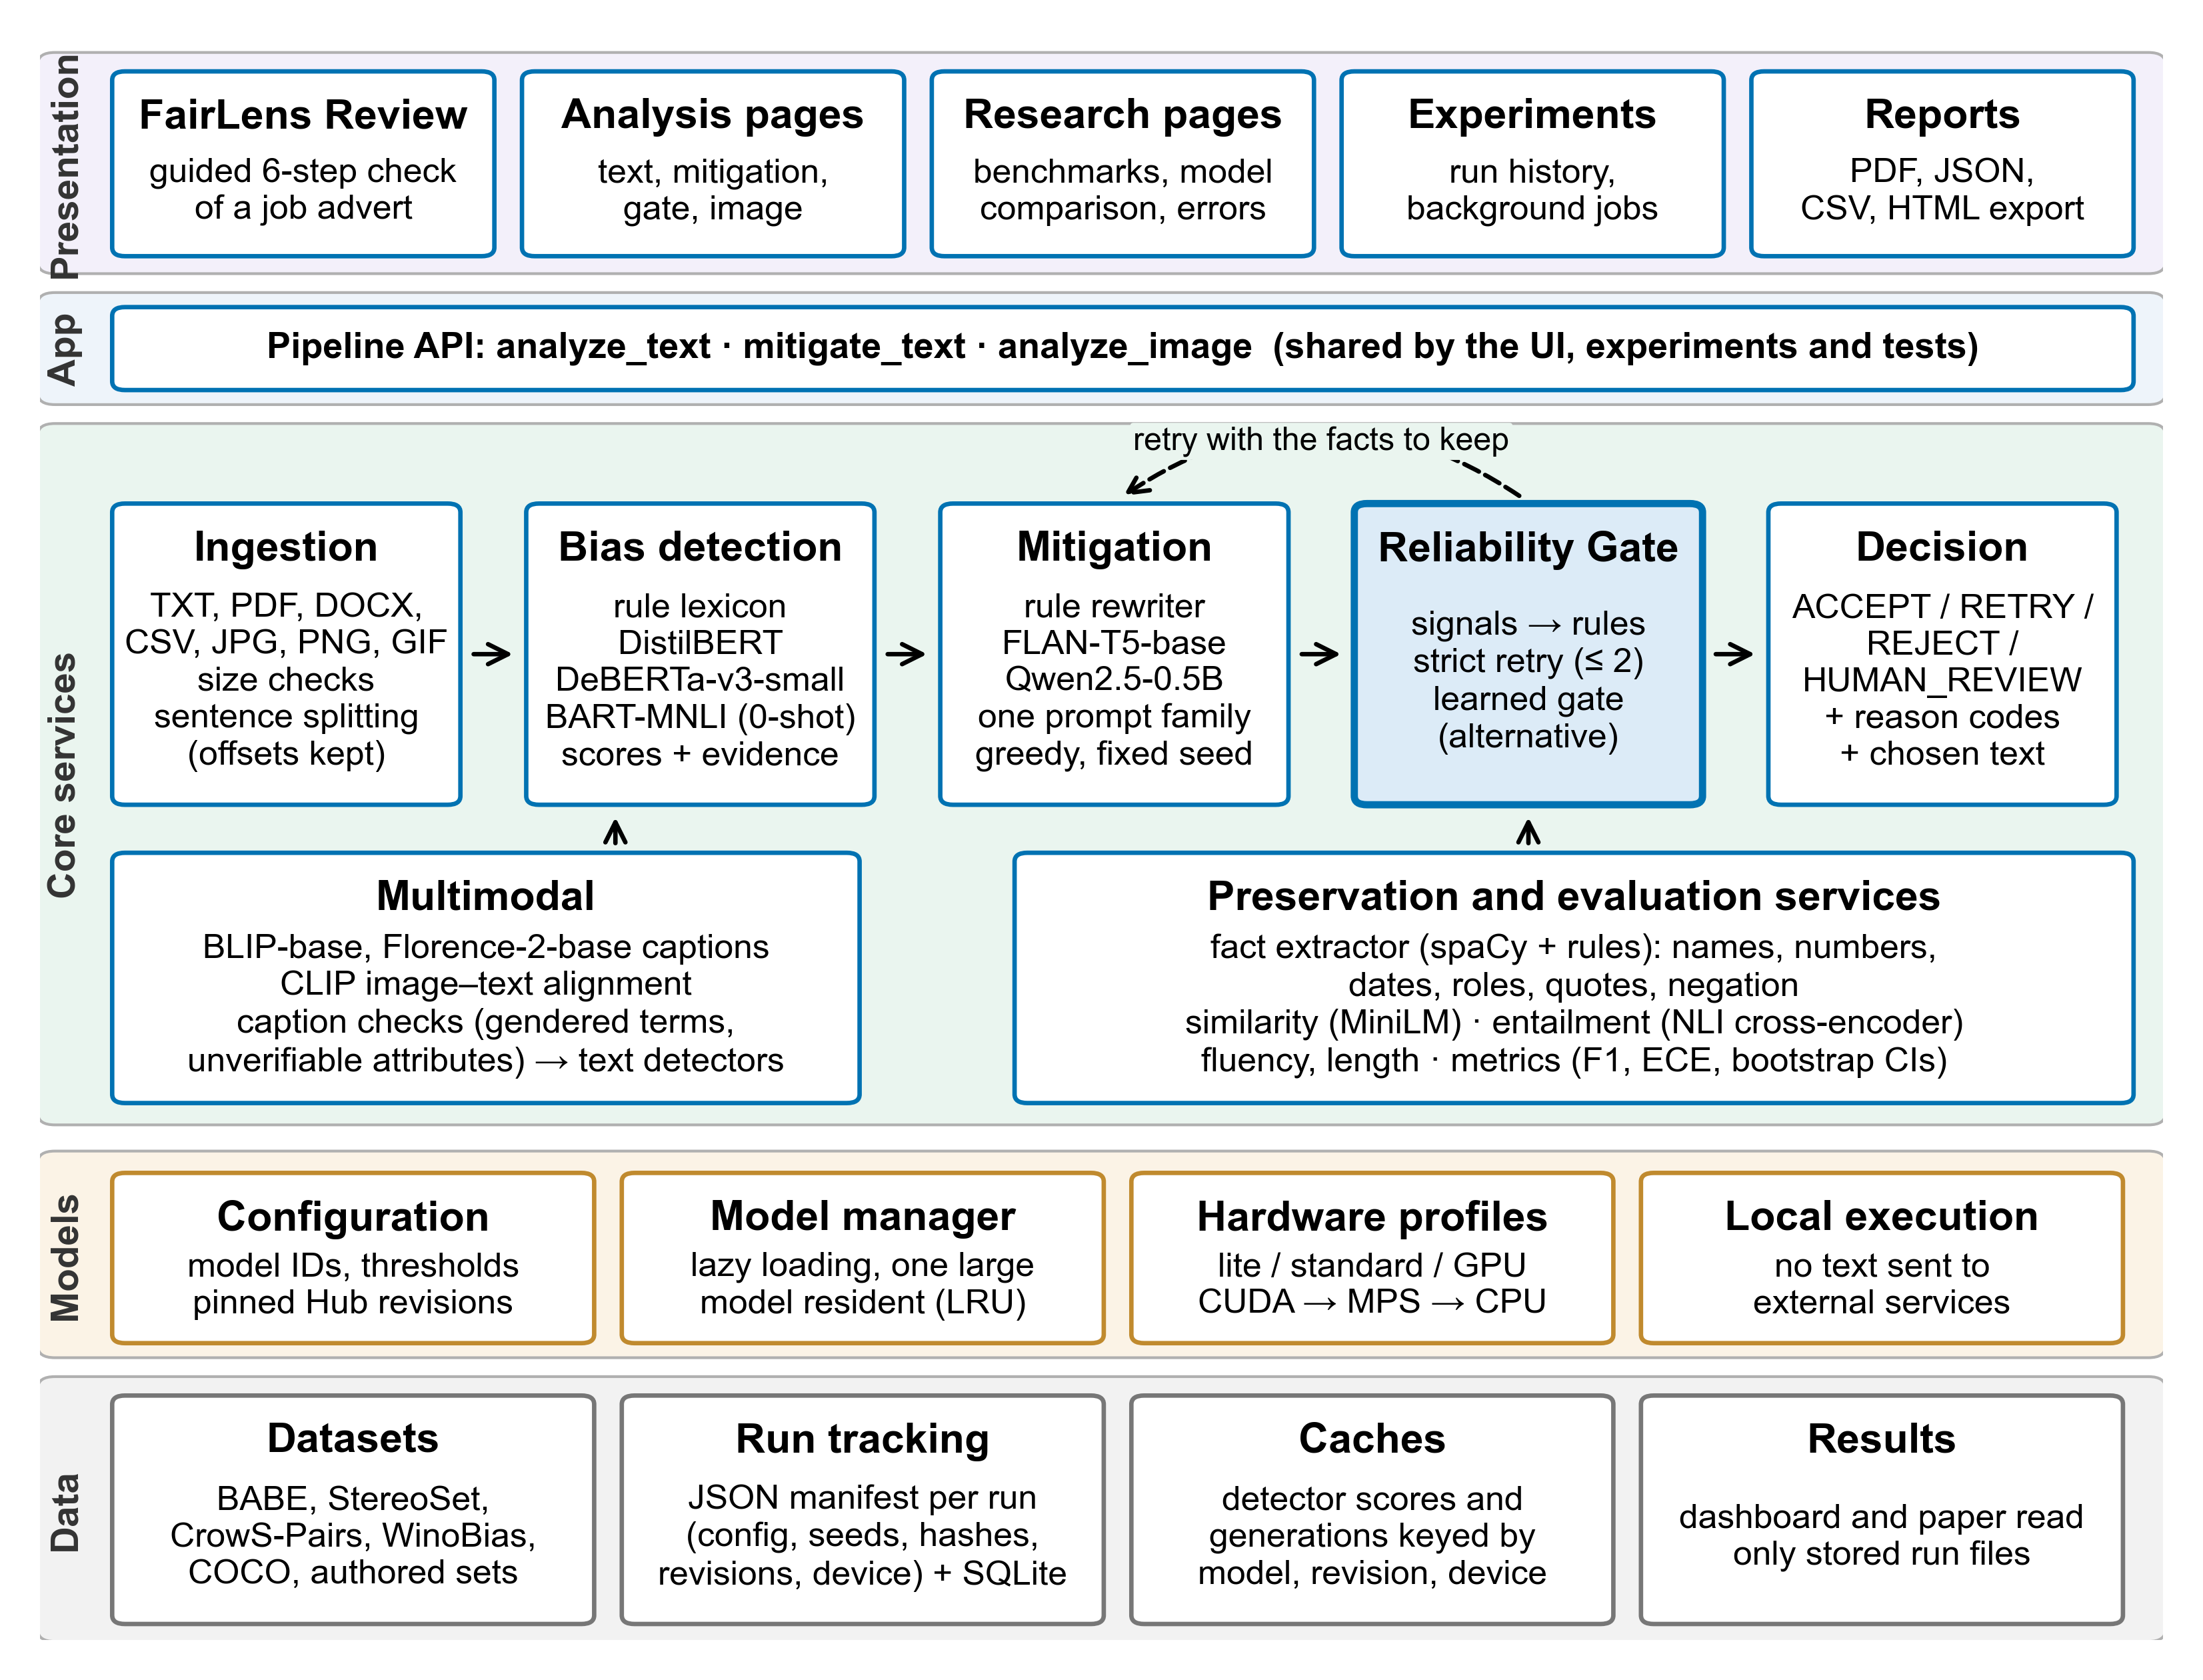
\includegraphics[width=0.95\textwidth]{figures/architecture.png}
\caption{High-level architecture of FairLens. The dashed arrow is the strict retry, which re-prompts the LLM rewriters
with the facts that must be kept.}
\label{fig:arch}
\end{figure}

The key features are:
\begin{itemize}
\item \textbf{Multi-detector bias detection} with highlighted phrases and per-detector scores.
\item \textbf{Three rewriters} (rule-based, FLAN-T5, Qwen2.5) shown side by side with a word-level diff view.
\item \textbf{Reliability Gate} with four verdicts and human-readable reason codes such as FACT\_LOSS or
UNNECESSARY\_CHANGE.
\item \textbf{Per-fact preservation checks} for names, numbers, dates, roles, quotations and negations.
\item \textbf{Caption analysis} for images using BLIP, Florence-2 and CLIP.
\item \textbf{Local, private processing} with automatic hardware profiles (lite, standard, GPU).
\item \textbf{Reproducibility}: every experiment stores a manifest with its configuration, seeds, dataset hashes and
pinned model revisions; the dashboard shows only stored results.
\end{itemize}

\section{Work Plan}
The work was carried out in seven phases (Table~\ref{tab:workplan}); the phases overlapped where implementation work
informed the review and vice versa.

\begin{longtable}{|c|L{4.3cm}|L{9cm}|}
\caption{Phase-wise work plan}\label{tab:workplan}\\
\hline
\textbf{Phase} & \textbf{Activity} & \textbf{Outcome}\\ \hline\endfirsthead
\hline \textbf{Phase} & \textbf{Activity} & \textbf{Outcome}\\ \hline\endhead
1 & Problem study and literature survey & Review of detection, rewriting, verification and AI-ethics literature;
research gaps identified; ethical requirements R1--R5 stated.\\ \hline
2 & Requirements and architecture & Functional and non-functional requirements; layered architecture; model registry
with pinned revisions; hardware profiles.\\ \hline
3 & Datasets & BABE, StereoSet, CrowS-Pairs unified into one schema with group-aware splits; WinoBias probe; 136
hand-written cases; mitigation set; controlled gate set.\\ \hline
4 & Detection & Rule lexicon; DistilBERT and DeBERTa-v3-small fine-tuning; BART-MNLI zero-shot template selection;
explanations by occlusion.\\ \hline
5 & Mitigation and Reliability Gate & Shared prompt family; rule rewriter; FLAN-T5 and Qwen2.5 adapters; signals,
transparent rules, strict retry, learned gates and baselines.\\ \hline
6 & Application & Twelve-page Streamlit dashboard; guided FairLens Review workflow; image analysis; report export;
background jobs; automated tests.\\ \hline
7 & Evaluation and documentation & Detection, mitigation, Gate and image benchmarks with bootstrap confidence
intervals and ablations; leakage check and re-split; research paper and project report.\\ \hline
\end{longtable}

\textbf{Organisation of the report.} Chapter~\ref{ch:lit} surveys the literature and identifies research gaps.
Chapter~\ref{ch:srs} specifies software and hardware requirements. Chapter~\ref{ch:method} describes the methodology,
tools, data and the formulae used by each stage. Chapter~\ref{ch:results} reports the experimental results and
discusses them. Chapter~\ref{ch:conc} concludes and lists future work.

% =====================================================================================
% CHAPTER 2
% =====================================================================================
\chapter{Literature Survey}\label{ch:lit}

\section{Overview}
This chapter surveys work relevant to automated bias mitigation. It is organised around four themes: detecting biased
language, neutralising and detoxifying rewrites, checking generated text and abstaining, and the ethics of automated
language intervention.

\subsection{Detecting Biased Language}
Sentence-level bias detection is trained and evaluated on benchmark datasets that operationalise bias in different
ways. BABE annotates media bias and loaded framing in news sentences \cite{babe}; StereoSet and CrowS-Pairs contrast
stereotypical and less stereotypical sentences about social groups \cite{stereoset,crows}; WinoBias tests
gender--occupation associations in coreference \cite{winobias}; BOLD measures bias in open-ended generation \cite{bold}.
These datasets are not interchangeable, and several contain validity problems: anti-stereotypical sentences often still
generalise about a group, and some items are inconsistent \cite{salmon}. Surveys stress that ``bias'' in NLP is often
under-specified \cite{blodgett2020,gallegos}. FairLens therefore reports detection per source and treats any detector
score as fallible evidence, not ground truth.

\subsection{Neutralising and Detoxifying Rewrites}
Pryzant et al.\ introduced the Wiki Neutrality Corpus and models that neutralise subjective bias in encyclopaedic text
\cite{pryzant}. Later work rewrites biased or sensitive text by detecting and perturbing biased tokens \cite{depen} or
rewrites gendered language into gender-neutral English \cite{theythem}. In detoxification, ParaDetox and ParaDeHate build
parallel corpora and check content preservation while constructing the data \cite{paradetox,paradehate}. LLM-guided
synthetic augmentation screens generated rewrites with similarity and attribute checks \cite{lgsa}.

\subsection{Checking Generated Text and Abstaining}
Natural language inference (NLI) models are used to detect factual inconsistency between a source and a generated text,
notably in summarisation \cite{summac}. LLMs are also used as judges of other models' outputs, with documented position
and self-preference biases \cite{mtbench}. Selective classification lets a model abstain when its confidence is low,
trading coverage for risk \cite{selective}, and conformal methods give distribution-free control of such risks
\cite{conformal}.

\subsection{Ethics of Automated Language Intervention}
Critiques of LLMs warn that fluent output invites unwarranted trust and that the costs of errors fall unevenly
\cite{parrots}. Principle-based frameworks converge on non-maleficence, autonomy, justice and explicability
\cite{floridi,jobin}, and the EU AI Act makes human oversight a legal requirement for high-risk uses such as recruitment
\cite{euaiact}. Captioning models have been shown to rely on gendered context rather than visual evidence
\cite{snowboard}, so the same concerns apply to multimodal systems.

\section{Detailed Survey}

\subsection{Review Methodology}
Candidate studies were identified in the ACL Anthology, IEEE Xplore, the ACM Digital Library, SpringerLink and arXiv
using combinations of the terms \emph{bias detection}, \emph{stereotype}, \emph{neutralisation}, \emph{debiasing
rewrite}, \emph{detoxification}, \emph{factual consistency}, \emph{NLI}, \emph{LLM-as-a-judge}, \emph{selective
prediction} and \emph{AI ethics}. Studies were included if they proposed a dataset, detector, rewriting method or
verification method for biased or harmful text, or a principle-level framework for responsible AI. For each study we
recorded the technique, the data, what is evaluated and the main limitation with respect to safe, verified mitigation.

\subsection{Comparison of Representative Studies}
Table~\ref{tab:survey} compares representative studies with the present system.

\begin{longtable}{|L{2.6cm}|L{3.2cm}|L{2.4cm}|L{2.8cm}|L{3.2cm}|}
\caption{Comparative Survey of Existing Bias Detection and Mitigation Work}\label{tab:survey}\\
\hline
\textbf{Study} & \textbf{Technique} & \textbf{Task} & \textbf{Evaluated on} & \textbf{Major limitation}\\ \hline\endfirsthead
\multicolumn{5}{l}{\small\textit{Table \thetable\ continued}}\\ \hline
\textbf{Study} & \textbf{Technique} & \textbf{Task} & \textbf{Evaluated on} & \textbf{Major limitation}\\ \hline\endhead
\hline \multicolumn{5}{r}{\small\textit{Continued on next page}}\\ \endfoot
\hline\endlastfoot
BABE \cite{babe} & Expert-annotated news sentences; distant supervision & Media-bias detection & Sentence
classification F1 & Detection only; news framing, not stereotypes\\ \hline
StereoSet \cite{stereoset} & Stereotype / anti-stereotype / unrelated triples & Bias measurement in LMs & Stereotype and
language-model scores & Known validity problems \cite{salmon}; no correction\\ \hline
CrowS-Pairs \cite{crows} & Minimal sentence pairs & Bias measurement in masked LMs & Preference for stereotypical
sentence & Pairs inconsistent in places \cite{salmon}; no correction\\ \hline
WinoBias \cite{winobias} & Pro- and anti-stereotypical coreference & Gender bias in coreference & Accuracy gap &
Coreference task; used here only as a false-alarm probe\\ \hline
WNC / neutralisation \cite{pryzant} & Seq2seq rewriting of subjective text & Bias neutralisation & BLEU, human
fluency/bias ratings & No check that facts survive; no abstention\\ \hline
DEPEN \cite{depen} & Detect biased tokens, perturb via gradient decoding & Neutral rewriting & Bias and fluency
metrics & No run-time decision layer\\ \hline
Gender-neutral rewriting \cite{theythem} & Rule + neural rewriting to singular ``they'' & Gender-neutral English & Word
error rate against references & Gender only; no preservation gate\\ \hline
ParaDetox \cite{paradetox} & Crowd-sourced parallel detox corpus & Detoxification & Style accuracy, similarity, fluency
& Toxicity, not stereotypes; checks only when building data\\ \hline
ParaDeHate \cite{paradehate} & LLM-in-the-loop parallel data & Hate-speech detoxification & Style transfer metrics &
No per-fact checks at run time\\ \hline
LGSA \cite{lgsa} & LLM-generated augmentations screened by similarity & Data augmentation for debiasing & Downstream
fairness metrics & No per-fact checks or multi-way decision\\ \hline
SummaC \cite{summac} & Sentence-level NLI for consistency & Summarisation consistency & Inconsistency detection
benchmarks & Not applied to bias rewrites\\ \hline
LLM-as-a-judge \cite{mtbench} & Strong LLM rates model outputs & Open-ended evaluation & Agreement with human
preferences & Position and self-preference bias; no explicit criteria\\ \hline
\textbf{FairLens (this work)} & Four detectors, three rewriters, rule-based Reliability Gate with reason codes,
caption extension & Detection, mitigation and verified acceptance & Shared test split, mitigation set, controlled gate set
with gold decisions, COCO captions & English only; small local rewriters; automatic evaluation of rewrites\\ \hline
\end{longtable}

\subsection{Comparative Analysis}
Three patterns stand out in Table~\ref{tab:survey}. First, detection and correction are studied separately: detectors
flag bias but do not propose fixes, and rewriters do not verify their own output. Second, every rewriting approach is
judged by bias or toxicity reduction and fluency, not by whether facts, negations and roles survive. Third, no approach
treats ``do not change this text'' or ``ask a person'' as a legitimate output, and no study compares selection policies
(lowest bias score, highest similarity, LLM judge) against each other on inputs with known correct decisions.

\section{Research Gap Identification}
From this review, five gaps stand out.

\begin{description}[style=nextline]
\item[G1 Detection without verified correction.] Detectors flag bias but do not propose and check fixes.
\item[G2 Bias score as the only criterion.] Rewriters are judged by bias reduction and fluency, not by whether facts,
negations and roles survive.
\item[G3 No abstention.] Rewriting systems always return an output; none defers uncertain cases to a person with
reasons.
\item[G4 Inconsistent evaluation.] Detectors are often reported on their own training source, with no false-alarm probe
or calibration, and selection policies are rarely compared.
\item[G5 Text-only scope.] Captions produced by vision--language models are rarely screened with the same tools.
\end{description}

\section{Mapping of Objectives with Research Gap Identification}
Table~\ref{tab:objgap} maps each project objective (Section 1.3) to the research gap it addresses and states how far
the gap is addressed in this work.

\begin{longtable}{|L{3.6cm}|c|L{9cm}|}
\caption{Mapping of Objectives to Research Gaps}\label{tab:objgap}\\
\hline
\textbf{Objective} & \textbf{Gap} & \textbf{How it is addressed, and its status}\\ \hline\endfirsthead
\hline \textbf{Objective} & \textbf{Gap} & \textbf{How it is addressed, and its status}\\ \hline\endhead
O1: Fair comparison of detectors & G4 & Five detectors evaluated on one held-out split with macro-F1, ROC-AUC, ECE and
bootstrap CIs, plus WinoBias false-alarm and CrowS-Pairs/StereoSet probes. Done.\\ \hline
O2: Rewriters on bias and preservation & G2 & Rule, FLAN-T5 and Qwen2.5 compared on bias reduction, similarity,
entailment, fact retention and unnecessary change. Done (automatic measures; no human rating yet).\\ \hline
O3: Reliability Gate & G1, G2, G3 & Transparent four-way Gate with reason codes, strict retry, learned-gate and
selection baselines, and per-signal ablations on a controlled set with gold decisions. Done.\\ \hline
O4: Caption extension & G5 & BLIP and Florence-2 captions checked with CLIP alignment, gendered-term and
unverifiable-attribute checks and the text detectors. Done on 80 COCO images.\\ \hline
O5: Reproducible local application & G4 & Run manifests, pinned model revisions, SQLite index; dashboard reads only
stored runs; cross-platform installers and automated tests. Done.\\ \hline
\end{longtable}

% =====================================================================================
% CHAPTER 3
% =====================================================================================
\chapter{Software and Hardware Requirement Specification}\label{ch:srs}

\section{Functional Requirements}
The functional requirements (FR) of the system are listed in Table~\ref{tab:fr}.

\begin{longtable}{|c|L{4cm}|L{9.2cm}|}
\caption{Functional Requirements}\label{tab:fr}\\
\hline
\textbf{ID} & \textbf{Requirement} & \textbf{Description}\\ \hline\endfirsthead
\hline \textbf{ID} & \textbf{Requirement} & \textbf{Description}\\ \hline\endhead
FR1 & Input and ingestion & Accept pasted text and TXT, PDF, DOCX, CSV and JPG/PNG/GIF uploads; validate type and size;
report truncation beyond 20,000 characters.\\ \hline
FR2 & Sentence segmentation & Split text into sentences with character offsets so every finding maps back to the
original document.\\ \hline
FR3 & Bias detection & Score every sentence with all available detectors; report the ensemble score, per-detector
scores and bias categories.\\ \hline
FR4 & Explanation & Highlight the phrases responsible for a detection (lexicon matches or occlusion attribution).\\ \hline
FR5 & Mitigation & Generate rule-based, FLAN-T5 and Qwen2.5 rewrites for biased sentences and show a word-level diff.\\ \hline
FR6 & Preservation checks & Compute semantic similarity, entailment, contradiction, fact retention, fluency and
length ratio for every candidate.\\ \hline
FR7 & Reliability Gate & Return ACCEPT, RETRY, REJECT or HUMAN\_REVIEW with reason codes; perform at most two strict
retries; select the best accepted candidate.\\ \hline
FR8 & Image analysis & Caption images with two captioners, measure image--caption alignment and run the caption
checks and text detectors.\\ \hline
FR9 & Research dashboard & Show benchmark, model-comparison and error-analysis results read only from stored run
files, each labelled with its run ID.\\ \hline
FR10 & Export & Export review results as PDF and JSON, and benchmark results as CSV/HTML.\\ \hline
FR11 & Experiment tracking & Record configuration, seeds, dataset hashes, model revisions, device and runtime for
every experiment.\\ \hline
\end{longtable}

\section{Non-functional Requirements}
\begin{itemize}
\item \textbf{Transparency and contestability:} every Gate verdict shall carry reason codes and the evidence behind
them, so that an author can check and dispute the decision.
\item \textbf{Fidelity:} the system shall never accept a rewrite that fails a preservation check, and shall never
change a sentence it does not judge biased.
\item \textbf{Honesty of results:} the dashboard shall display only numbers read from stored run files; illustrative
examples shall be labelled as such (enforced by an automated test).
\item \textbf{Privacy:} all processing shall run locally; uploaded text shall not be stored and shall never alter the
benchmark results.
\item \textbf{Reproducibility:} all dependencies and model revisions shall be pinned; seeds shall be fixed; every run
shall write a manifest.
\item \textbf{Performance and resource use:} the system shall run on an ordinary laptop without a GPU, loading models
lazily and keeping at most one large model resident.
\item \textbf{Portability:} the system shall run on Windows, macOS and Linux with installer scripts for each.
\item \textbf{Usability:} a guided six-step review shall lead non-expert users from input to decision, with light and
dark themes.
\item \textbf{Testability:} pipeline logic and every dashboard page shall be covered by automated tests that can run
with lightweight stand-ins for the neural models.
\end{itemize}

\section{Hardware Requirements}
The system was built so that every model runs on a CPU; a GPU (CUDA) or Apple Silicon (MPS) is used automatically when
present. Table~\ref{tab:hw} lists the recommended configuration. These are the configurations on which the project was
developed and run, not benchmarked minimums.

\begin{longtable}{|L{4cm}|L{10.2cm}|}
\caption{Hardware Requirements (Recommended)}\label{tab:hw}\\
\hline
\textbf{Component} & \textbf{Requirement}\\ \hline\endfirsthead
\hline \textbf{Component} & \textbf{Requirement}\\ \hline\endhead
Processor & Multi-core x86-64 or Apple Silicon CPU; GPU optional. Development and training used an Apple M4 laptop
(MPS backend); the Gate re-runs used a Windows laptop on CPU.\\ \hline
Memory & 16\,GB RAM recommended. A ``lite'' profile (DistilBART-MNLI, FLAN-T5-small) is selected automatically on
smaller machines.\\ \hline
Storage & About 25\,GB free disk: about 12\,GB for the downloaded and verified models, plus datasets, checkpoints and
run outputs.\\ \hline
Network & Internet access only for the first download of models and datasets; analysis runs offline.\\ \hline
Client & Any modern web browser on the same machine (or local network).\\ \hline
\end{longtable}

\section{Software Requirements}
Table~\ref{tab:sw} lists the implementation stack. The source package comprises about 6,500 lines of Python (of which
about 2,300 are the dashboard), and the test suite about 2,100 lines.

\begin{longtable}{|L{3.6cm}|L{10.6cm}|}
\caption{Implementation Stack}\label{tab:sw}\\
\hline
\textbf{Component} & \textbf{Implementation}\\ \hline\endfirsthead
\hline \textbf{Component} & \textbf{Implementation}\\ \hline\endhead
Language & Python 3.11 (all dependencies pinned).\\ \hline
Deep learning & PyTorch 2.14.1; Hugging Face Transformers 5.20.2; sentence-transformers.\\ \hline
Detectors & Rule lexicon; DistilBERT \cite{distilbert} and DeBERTa-v3-small \cite{debertav3} fine-tuned; BART-large-MNLI
\cite{bart} zero-shot \cite{yin}; public RoBERTa (BABE-trained) as reference.\\ \hline
Rewriters & Rule rewriter; FLAN-T5-base \cite{flant5}; Qwen2.5-0.5B-Instruct \cite{qwen}.\\ \hline
Preservation & all-MiniLM-L6-v2 sentence embeddings \cite{sbert,minilm}; NLI cross-encoder (DeBERTa-v3-small); spaCy
3.8.16 for fact extraction.\\ \hline
Multimodal & BLIP-base \cite{blip}, Florence-2-base \cite{florence}, CLIP ViT-B/32 \cite{clip}.\\ \hline
Machine learning & scikit-learn (learned gates, metrics).\\ \hline
User interface & Streamlit 1.66.1; Plotly charts.\\ \hline
Storage and tracking & JSON run manifests, Parquet datasets, SQLite run index, score and generation caches.\\ \hline
Testing & pytest suite (246 tests) plus a browser smoke test of the review flow.\\ \hline
\end{longtable}

\section{Cost Estimation}
The system is built entirely from open-source components and openly licensed models (Table~\ref{tab:cost}). Because
all models run locally, there is no per-request API cost.

\begin{longtable}{|L{5.4cm}|L{8.8cm}|}
\caption{Cost Components}\label{tab:cost}\\
\hline
\textbf{Item} & \textbf{Cost basis}\\ \hline\endfirsthead
\hline \textbf{Item} & \textbf{Cost basis}\\ \hline\endhead
Python, PyTorch, Transformers, sentence-transformers, spaCy, scikit-learn, Streamlit, Plotly & Open source; no licence
cost.\\ \hline
Pre-trained models (DistilBERT, DeBERTa-v3, BART-MNLI, FLAN-T5, Qwen2.5, MiniLM, BLIP, Florence-2, CLIP) & Openly
licensed on the Hugging Face Hub; free download.\\ \hline
Datasets (BABE, StereoSet, CrowS-Pairs, WinoBias, COCO) & Free for research use under their licences (BABE:
non-commercial only).\\ \hline
External APIs & None; no text is sent to a hosted service.\\ \hline
Development hardware & Team's existing laptops; no paid cloud compute was used.\\ \hline
Hosting & Not incurred; the application runs locally.\\ \hline
\end{longtable}

% =====================================================================================
% CHAPTER 4
% =====================================================================================
\chapter{Methodology}\label{ch:method}

\section{Tools and Techniques}
\textbf{Tools.} The stack is summarised in Table~\ref{tab:sw}. Models are loaded from the Hugging Face Hub, each pinned
to a specific commit recorded in a model lock file, and are managed by a model manager that loads them lazily, keeps one
large model in memory at a time and evicts the least recently used. Hardware is detected at start-up and a profile is
chosen (lite, standard or GPU); the device is selected in the order CUDA, Apple MPS, CPU.

\textbf{Techniques.} The methodology combines the following techniques, each described in Section~\ref{sec:details}.
\begin{itemize}
\item Offset-preserving sentence segmentation aware of quotations and abbreviations.
\item An ensemble of a rule lexicon, two fine-tuned transformer classifiers and a zero-shot NLI classifier.
\item Leave-one-word-out occlusion to explain transformer detections.
\item Rule-based and LLM rewriting from one shared prompt family, with greedy, seeded decoding.
\item Preservation signals: sentence-embedding similarity, bidirectional NLI entailment, contradiction, rule- and
spaCy-based fact extraction, fluency heuristics.
\item A transparent, ordered rule Gate with reason codes and a strict retry; learned gates as alternatives.
\item Caption generation and image--text alignment for images.
\item Bootstrap confidence intervals and paired-bootstrap ablations for evaluation.
\end{itemize}

\section{Data Set With Explanation}
Table~\ref{tab:data} lists the data.

\textbf{Detection data.} BABE \cite{babe}, StereoSet (intra- and inter-sentence) \cite{stereoset} and CrowS-Pairs
\cite{crows} were unified into one binary schema (1 = the sentence expresses or relies on a stereotype or biased
framing under the source's own annotation). Splits (70/15/15, seed 42) were made by group, so that the two members of a
minimal pair never fall into different splits, giving 10,365 training, 2,119 validation and 2,652 test sentences.
WinoBias \cite{winobias} was used only as a false-alarm probe: all its sentences are neutral, so any flag is a false
alarm. The Wiki Neutrality Corpus \cite{pryzant} could not be obtained (its host was unreachable and the only mirror is
gated).

\textbf{Mitigation data.} We hand-wrote 136 sentences with fictional names (91 biased, 45 neutral) covering recruitment
text, gender, age, race, religion, disability and socioeconomic stereotypes and media framing, deliberately including
names, numbers, dates, negations, roles and quotations; each biased sentence has one reference rewrite. Together with 140
sentences from the test split of the detection benchmarks they form a mitigation set of 276 inputs (211 biased, 65
neutral).

\textbf{Controlled gate set.} To evaluate the Gate against known correct answers, for each biased input the reference
rewrite is labelled ACCEPT, the unchanged original RETRY and seeded perturbations of the reference REJECT (number
changed, negation flipped, entity swapped, role swapped, antonym, hallucinated addition, truncation, altered quotation);
for each neutral input the unchanged original is ACCEPT and any change is REJECT. Three perturbation seeds give 2,481
candidates. The split into validation and test is made by source sentence, so all seeds of a sentence fall in the same
half. The test split has 68 sentences, giving 204 inputs (69 neutral) and 1,218 candidates.

\textbf{Image data.} 80 COCO val2017 images \cite{coco} (60 with people, 20 without), each with five human reference
captions.

\begin{longtable}{|L{3.2cm}|L{2.4cm}|L{2.4cm}|L{2.4cm}|L{3.6cm}|}
\caption{Datasets Used in the Evaluation}\label{tab:data}\\
\hline
\textbf{Dataset} & \textbf{Licence} & \textbf{Used for} & \textbf{Size used} & \textbf{Label meaning}\\ \hline\endfirsthead
\hline \textbf{Dataset} & \textbf{Licence} & \textbf{Used for} & \textbf{Size used} & \textbf{Label meaning}\\ \hline\endhead
BABE \cite{babe} & CC BY-NC-SA 4.0 & Detection & 4,118 sentences & Expert-labelled media bias in news\\ \hline
StereoSet \cite{stereoset} & CC BY-SA 4.0 & Detection, probe & 8,440 sentences & Stereotype = 1, anti-stereotype = 0\\ \hline
CrowS-Pairs \cite{crows} & CC BY-SA 4.0 & Detection, probe & 2,578 sentences & More stereotypical sentence = 1\\ \hline
WinoBias \cite{winobias} & MIT & False-alarm probe & 1,584 sentences & All neutral; any flag is a false alarm\\ \hline
Authored cases (this work) & -- & Mitigation, Gate & 136 sentences & 91 biased, 45 neutral, with reference rewrites\\ \hline
Mitigation set & Derived & Mitigation & 276 inputs & 211 biased, 65 neutral\\ \hline
Controlled gate set & Derived & Gate & 2,481 candidates & Gold ACCEPT / RETRY / REJECT by construction\\ \hline
COCO val2017 subset \cite{coco} & CC BY 4.0 + Flickr & Captions & 80 images & 60 with people, 20 without; 5 human captions each\\ \hline
\end{longtable}

\section{Flow Chart Of Methodology From Start To End}
Figure~\ref{fig:arch} shows the overall flow from an uploaded document to a decision, and Figure~\ref{fig:gate} shows
how the Reliability Gate decides for one candidate rewrite. In brief: (1) the input is loaded and segmented into
sentences; (2) every sentence is scored by the detectors; (3) sentences judged biased are rewritten by the three
rewriters, while the unchanged original is always kept as a candidate; (4) the preservation and bias signals are
computed for every candidate; (5) the Gate applies its rules and returns a verdict with reason codes, retrying the LLMs
with a stricter prompt at most twice; (6) the best accepted candidate, or a deferral to human review, is shown to the
user together with the evidence and can be exported.

\begin{figure}[H]
\centering
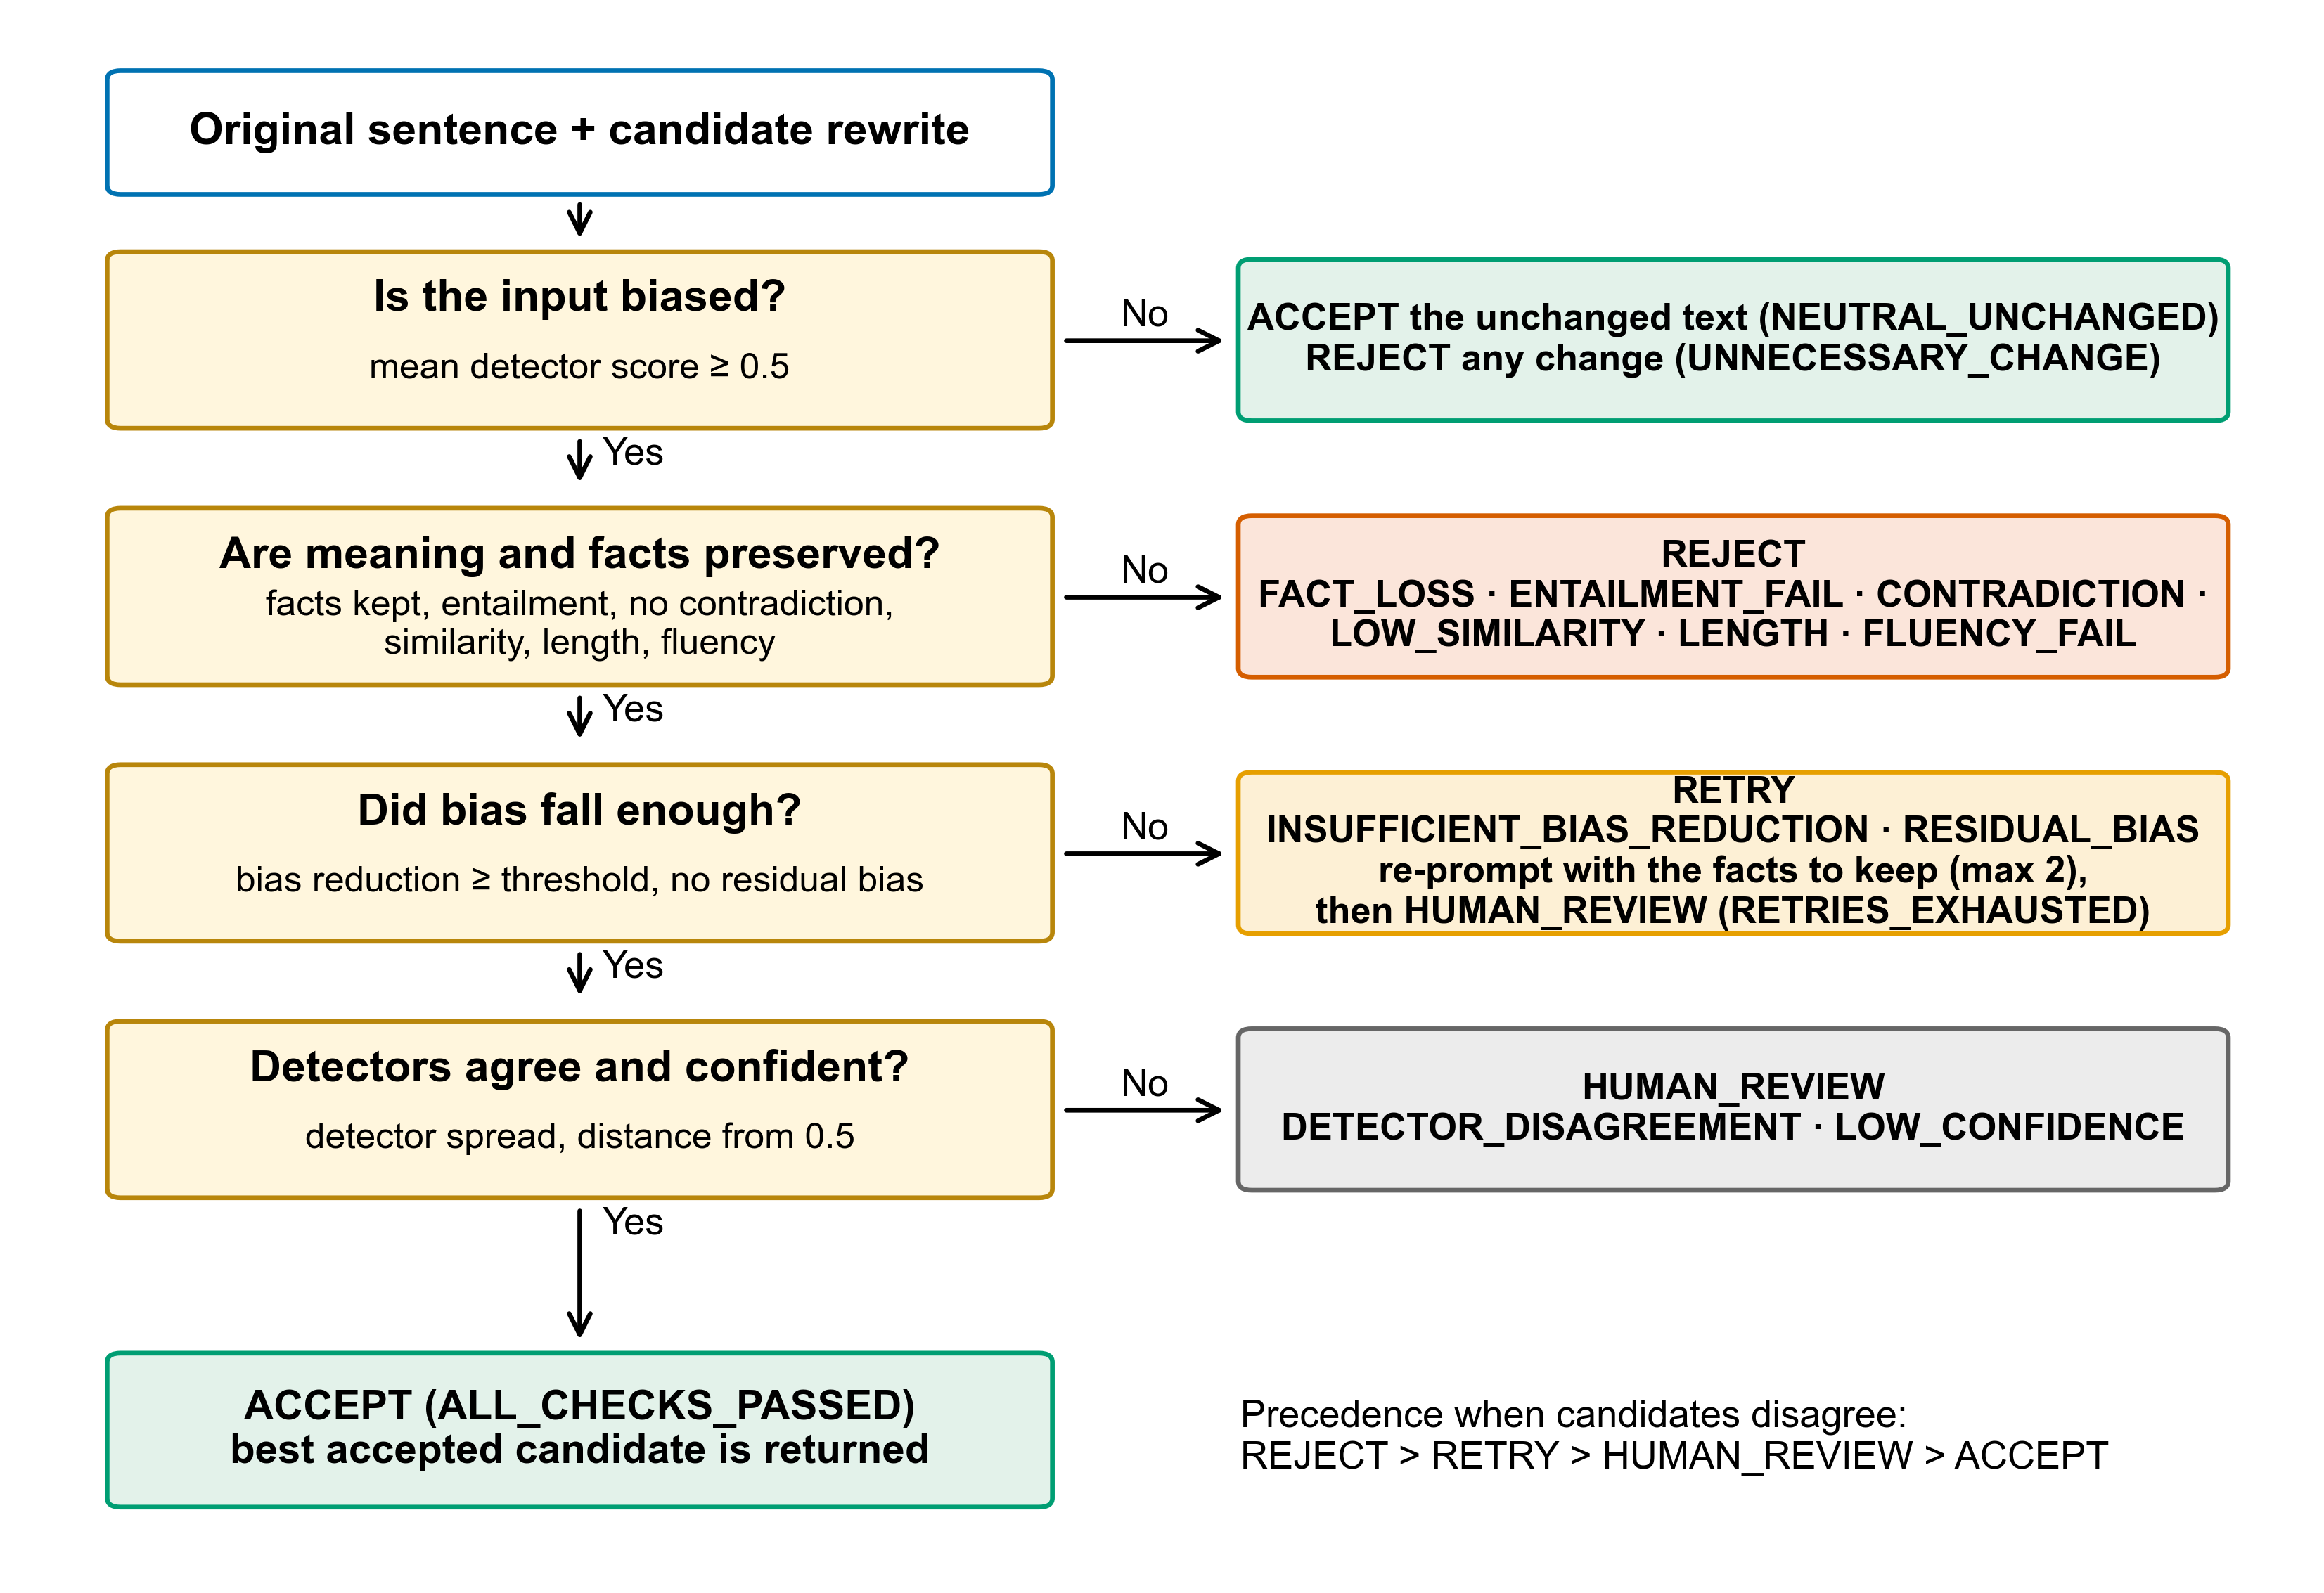
\includegraphics[width=0.95\textwidth]{figures/gate_flow.png}
\caption{Decision flow of the transparent rule Gate for one candidate rewrite, with the reason codes attached to each
outcome. Verdicts over several candidates are combined with the precedence REJECT $>$ RETRY $>$ HUMAN\_REVIEW $>$ ACCEPT.}
\label{fig:gate}
\end{figure}

\section{Explanation Of Methodology In Details With Equations And Formulae}\label{sec:details}
The architecture of Figure~\ref{fig:arch} is described stage by stage below, with the formulae that each stage
implements.

\subsection{Ingestion and Segmentation}
Each loader checks file type and size (10\,MB per file, 60 megapixels per image) and analyses at most 20,000
characters, reporting any truncation. Text is split into sentences $s_1,\dots,s_n$ by an offset-preserving segmenter, so
that each sentence $s_i$ carries its start and end character offsets $(a_i,b_i)$ in the original document and every
flagged phrase and rewrite can be mapped back to its exact position.

\subsection{Bias Detection}
Let $D=\{d_1,\dots,d_m\}$ be the available detectors, each returning a probability $p_j(s)\in[0,1]$ that sentence $s$ is
biased. The fine-tuned classifiers return the softmax probability of the ``biased'' class. The zero-shot detector
compares the entailment of a ``biased'' and a ``neutral'' hypothesis $h_b,h_n$:
\begin{equation}
p_{\text{zs}}(s)=\frac{\exp z_{\text{ent}}(s,h_b)}{\exp z_{\text{ent}}(s,h_b)+\exp z_{\text{ent}}(s,h_n)}
\end{equation}
The pipeline's bias score is the mean of the detector scores, and their spread measures disagreement:
\begin{equation}
B(s)=\frac{1}{m}\sum_{j=1}^{m}p_j(s),\qquad \sigma(s)=\sqrt{\frac{1}{m}\sum_{j=1}^{m}\big(p_j(s)-B(s)\big)^2}
\end{equation}
A sentence is judged biased when $B(s)\ge\tau_b$, with $\tau_b=0.5$.

\subsection{Explanation by Occlusion}
For a transformer detector $d$ and a sentence $s=w_1\dots w_k$, the importance of word $w_t$ is the drop in score when
it is removed:
\begin{equation}
\Delta_t = p_d(s) - p_d(s\setminus w_t)
\end{equation}
The words with the largest $\Delta_t$ are highlighted; for the rule detector, the lexicon matches are highlighted with
their category and strength.

\subsection{Mitigation}
For each biased sentence $x$, the candidate set is $C(x)=\{x, r_{\text{rule}}(x), r_{\text{flan}}(x),
r_{\text{qwen}}(x)\}$; the unchanged original is always a candidate, because for a sentence that is not biased the
correct action is to change nothing. Both LLMs receive the same instruction from one prompt family. Decoding is greedy
with at most 96 new tokens, a repetition penalty of 1.1 and a fixed seed. A strict retry re-prompts the LLMs with the
list of extracted facts that must be kept.

\subsection{Reliability Gate Signals}
For an original $x$ and candidate $c$ the Gate computes:
\begin{align}
\text{Bias reduction:}\quad & \Delta B = B(x)-B(c)\\
\text{Semantic similarity:}\quad & \text{sim}(x,c)=\frac{\mathbf{e}_x\cdot\mathbf{e}_c}{\lVert\mathbf{e}_x\rVert\,\lVert\mathbf{e}_c\rVert}\\
\text{Entailment:}\quad & E_{\rightarrow}=P(x\Rightarrow c),\qquad E_{\leftrightarrow}=\min\big(P(x\Rightarrow c),P(c\Rightarrow x)\big)\\
\text{Contradiction:}\quad & K=\max\big(P_{\text{con}}(x,c),P_{\text{con}}(c,x)\big)\\
\text{Fact retention:}\quad & F=\frac{|\,\text{facts}(x)\cap\text{facts}(c)\,|}{|\,\text{facts}(x)\,|}\quad(F=1\text{ if facts}(x)=\varnothing)\\
\text{Confidence margin:}\quad & M=2\,|B(c)-0.5|\\
\text{Uncertainty:}\quad & U=0.5\min\!\Big(1,\frac{\sigma(c)}{0.5}\Big)+0.5\,(1-M)
\end{align}
where $\mathbf{e}$ are all-MiniLM-L6-v2 sentence embeddings, $P(\cdot\Rightarrow\cdot)$ and $P_{\text{con}}$ come from
an NLI cross-encoder, and $\text{facts}(\cdot)$ are the named entities, numbers, dates, roles, quotations and negation
polarity extracted with spaCy and rules. Fluency is checked heuristically (repetition, prompt leakage, non-alphabetic
text) and the length ratio $|c|/|x|$ must lie in $[0.5,2.0]$.

\subsection{Reliability Gate Rules}
The rules are applied in a fixed order (Figure~\ref{fig:gate}):
\begin{enumerate}
\item If $B(x)<\tau_b$ (input not biased): accept $c=x$ (NEUTRAL\_UNCHANGED) and reject any change
(UNNECESSARY\_CHANGE).
\item If any preservation check fails ($F<1$, entailment below threshold, $K>0.5$, similarity below threshold, length
or fluency failure): REJECT with the corresponding reason codes.
\item If meaning is preserved but $\Delta B<\delta$ or $B(c)\ge 0.5$: RETRY with a strict prompt (at most two retries),
then HUMAN\_REVIEW.
\item If $\sigma(c)>\sigma_{\max}$ or $M<0.10$: HUMAN\_REVIEW (DETECTOR\_DISAGREEMENT or LOW\_CONFIDENCE).
\item Otherwise: ACCEPT (ALL\_CHECKS\_PASSED).
\end{enumerate}
Among several accepted candidates, the one with the highest $\Delta B+\text{sim}+F$ is returned. The default thresholds
were set a priori: minimum similarity 0.70, bidirectional entailment 0.50, minimum bias reduction $\delta=0.15$ and
$\sigma_{\max}=0.35$. They were then tuned on the validation split of the controlled set only, giving minimum
similarity 0.60, forward entailment $E_{\rightarrow}\ge0.70$ and $\delta=0.05$, with $\sigma_{\max}$ raised to 1.0
(which switches the disagreement check off, because the standard deviation of probabilities cannot exceed 0.5). The
tuned values were frozen before any test evaluation and are used by the application.

\subsection{Learned Gates and Baselines}
As less transparent alternatives, a logistic regression and a depth-4 decision tree are trained on 14 signal features of
the validation candidates; they defer to a person when their top class probability is below 0.6. The baselines are:
choose the lowest bias score; choose the changed candidate with the highest similarity; keep the original; always take
the first model's output; random choice (five seeds); and an LLM-as-judge in which Qwen2.5-0.5B-Instruct is asked whether
a changed candidate preserves the meaning.

\subsection{Multimodal Extension}
For an image $I$ and caption $t$, alignment is the CLIP cosine similarity
\begin{equation}
\text{CLIP}(I,t)=\frac{\mathbf{v}_I\cdot\mathbf{u}_t}{\lVert\mathbf{v}_I\rVert\,\lVert\mathbf{u}_t\rVert}
\end{equation}
Captions are generated with BLIP-base and Florence-2-base, checked for gendered terms and for attributes that pixels
cannot normally verify (such as nationality, wealth or religion), and passed to the same text detectors.

\subsection{Evaluation Metrics}
\textbf{Detection.} With true positives $TP$, false positives $FP$ and false negatives $FN$:
\begin{equation}
P=\frac{TP}{TP+FP},\qquad R=\frac{TP}{TP+FN},\qquad F_1=\frac{2PR}{P+R},\qquad \text{Macro-}F_1=\tfrac{1}{2}\big(F_1^{(0)}+F_1^{(1)}\big)
\end{equation}
together with ROC-AUC and the expected calibration error over 10 equal-width bins $B_k$ \cite{guo}:
\begin{equation}
\text{ECE}=\sum_{k=1}^{10}\frac{|B_k|}{N}\,\big|\,\text{acc}(B_k)-\text{conf}(B_k)\,\big|
\end{equation}
The WinoBias false-positive rate is the share of (neutral) WinoBias sentences with $B(s)\ge0.5$.

\textbf{Gate.} At the candidate level, three-class macro-F1 and the unsafe-accept rate
\begin{equation}
\text{UA}=P(\text{verdict}=\text{ACCEPT}\mid\text{gold}\neq\text{ACCEPT})
\end{equation}
At the input level, a selection is acceptable if its gold label is ACCEPT and harmful otherwise, split into keeping a
biased original (gold RETRY) and choosing a damaging rewrite (gold REJECT); the deferral rate and the unnecessary-change
rate on neutral inputs are also reported.

\textbf{Statistics.} Confidence intervals are 95\% percentile bootstrap intervals over test items (1,000 resamples);
differences between policies and ablations use the paired bootstrap. Seeds were fixed for splitting and training (42),
generation (13), perturbations (11, 22, 33) and random baselines (100--104).

% =====================================================================================
% CHAPTER 5
% =====================================================================================
\chapter{Results and Discussion}\label{ch:results}
This chapter reports the results of the completed experiment runs. Every number below was read from the stored run
files; nothing was entered by hand.

\section{Bias Detection}
Table~\ref{tab:det} and Figure~\ref{fig:detf1} summarise detection on the 2,652 test sentences. Fine-tuned
DeBERTa-v3-small was the strongest detector (macro-F1 0.814, 95\% CI 0.800--0.828) and the most consistent across
sources (0.811--0.817), followed by DistilBERT (0.777). The public RoBERTa classifier scored highest on BABE (0.853), the
source it was trained on, but at or below 0.544 on the stereotype datasets. Zero-shot BART-MNLI reached 0.611 and the
rule baseline 0.354, with very low recall (0.035).

\begin{longtable}{|L{3.4cm}|c|c|L{2.4cm}|c|c|L{1.9cm}|}
\caption{Detection on the Shared Test Split ($n$ = 2,652, Threshold 0.5)}\label{tab:det}\\
\hline
\textbf{Detector} & \textbf{Prec.} & \textbf{Rec.} & \textbf{Macro-F1 [95\% CI]} & \textbf{ROC-AUC} & \textbf{ECE} &
\textbf{WinoBias FPR (pro / anti)}\\ \hline\endfirsthead
\hline \textbf{Detector} & \textbf{Prec.} & \textbf{Rec.} & \textbf{Macro-F1 [95\% CI]} & \textbf{ROC-AUC} & \textbf{ECE} &
\textbf{WinoBias FPR (pro / anti)}\\ \hline\endhead
Rule-based & 0.557 & 0.035 & 0.354 [0.342, 0.369] & 0.515 & 0.491 & 0.000 / 0.000\\ \hline
DistilBERT (fine-tuned) & 0.775 & 0.810 & 0.777 [0.762, 0.791] & 0.856 & 0.122 & 0.441 / 0.428\\ \hline
DeBERTa-v3-small (fine-tuned) & 0.818 & 0.829 & \textbf{0.814} [0.800, 0.828] & 0.896 & 0.123 & 0.396 / 0.376\\ \hline
BART-MNLI (zero-shot) & 0.620 & 0.674 & 0.611 [0.593, 0.629] & 0.648 & 0.105 & 0.417 / 0.427\\ \hline
Public RoBERTa (BABE-trained) & 0.701 & 0.564 & 0.646 [0.627, 0.661] & 0.722 & 0.243 & 0.054 / 0.062\\ \hline
\end{longtable}

\begin{figure}[H]
\centering
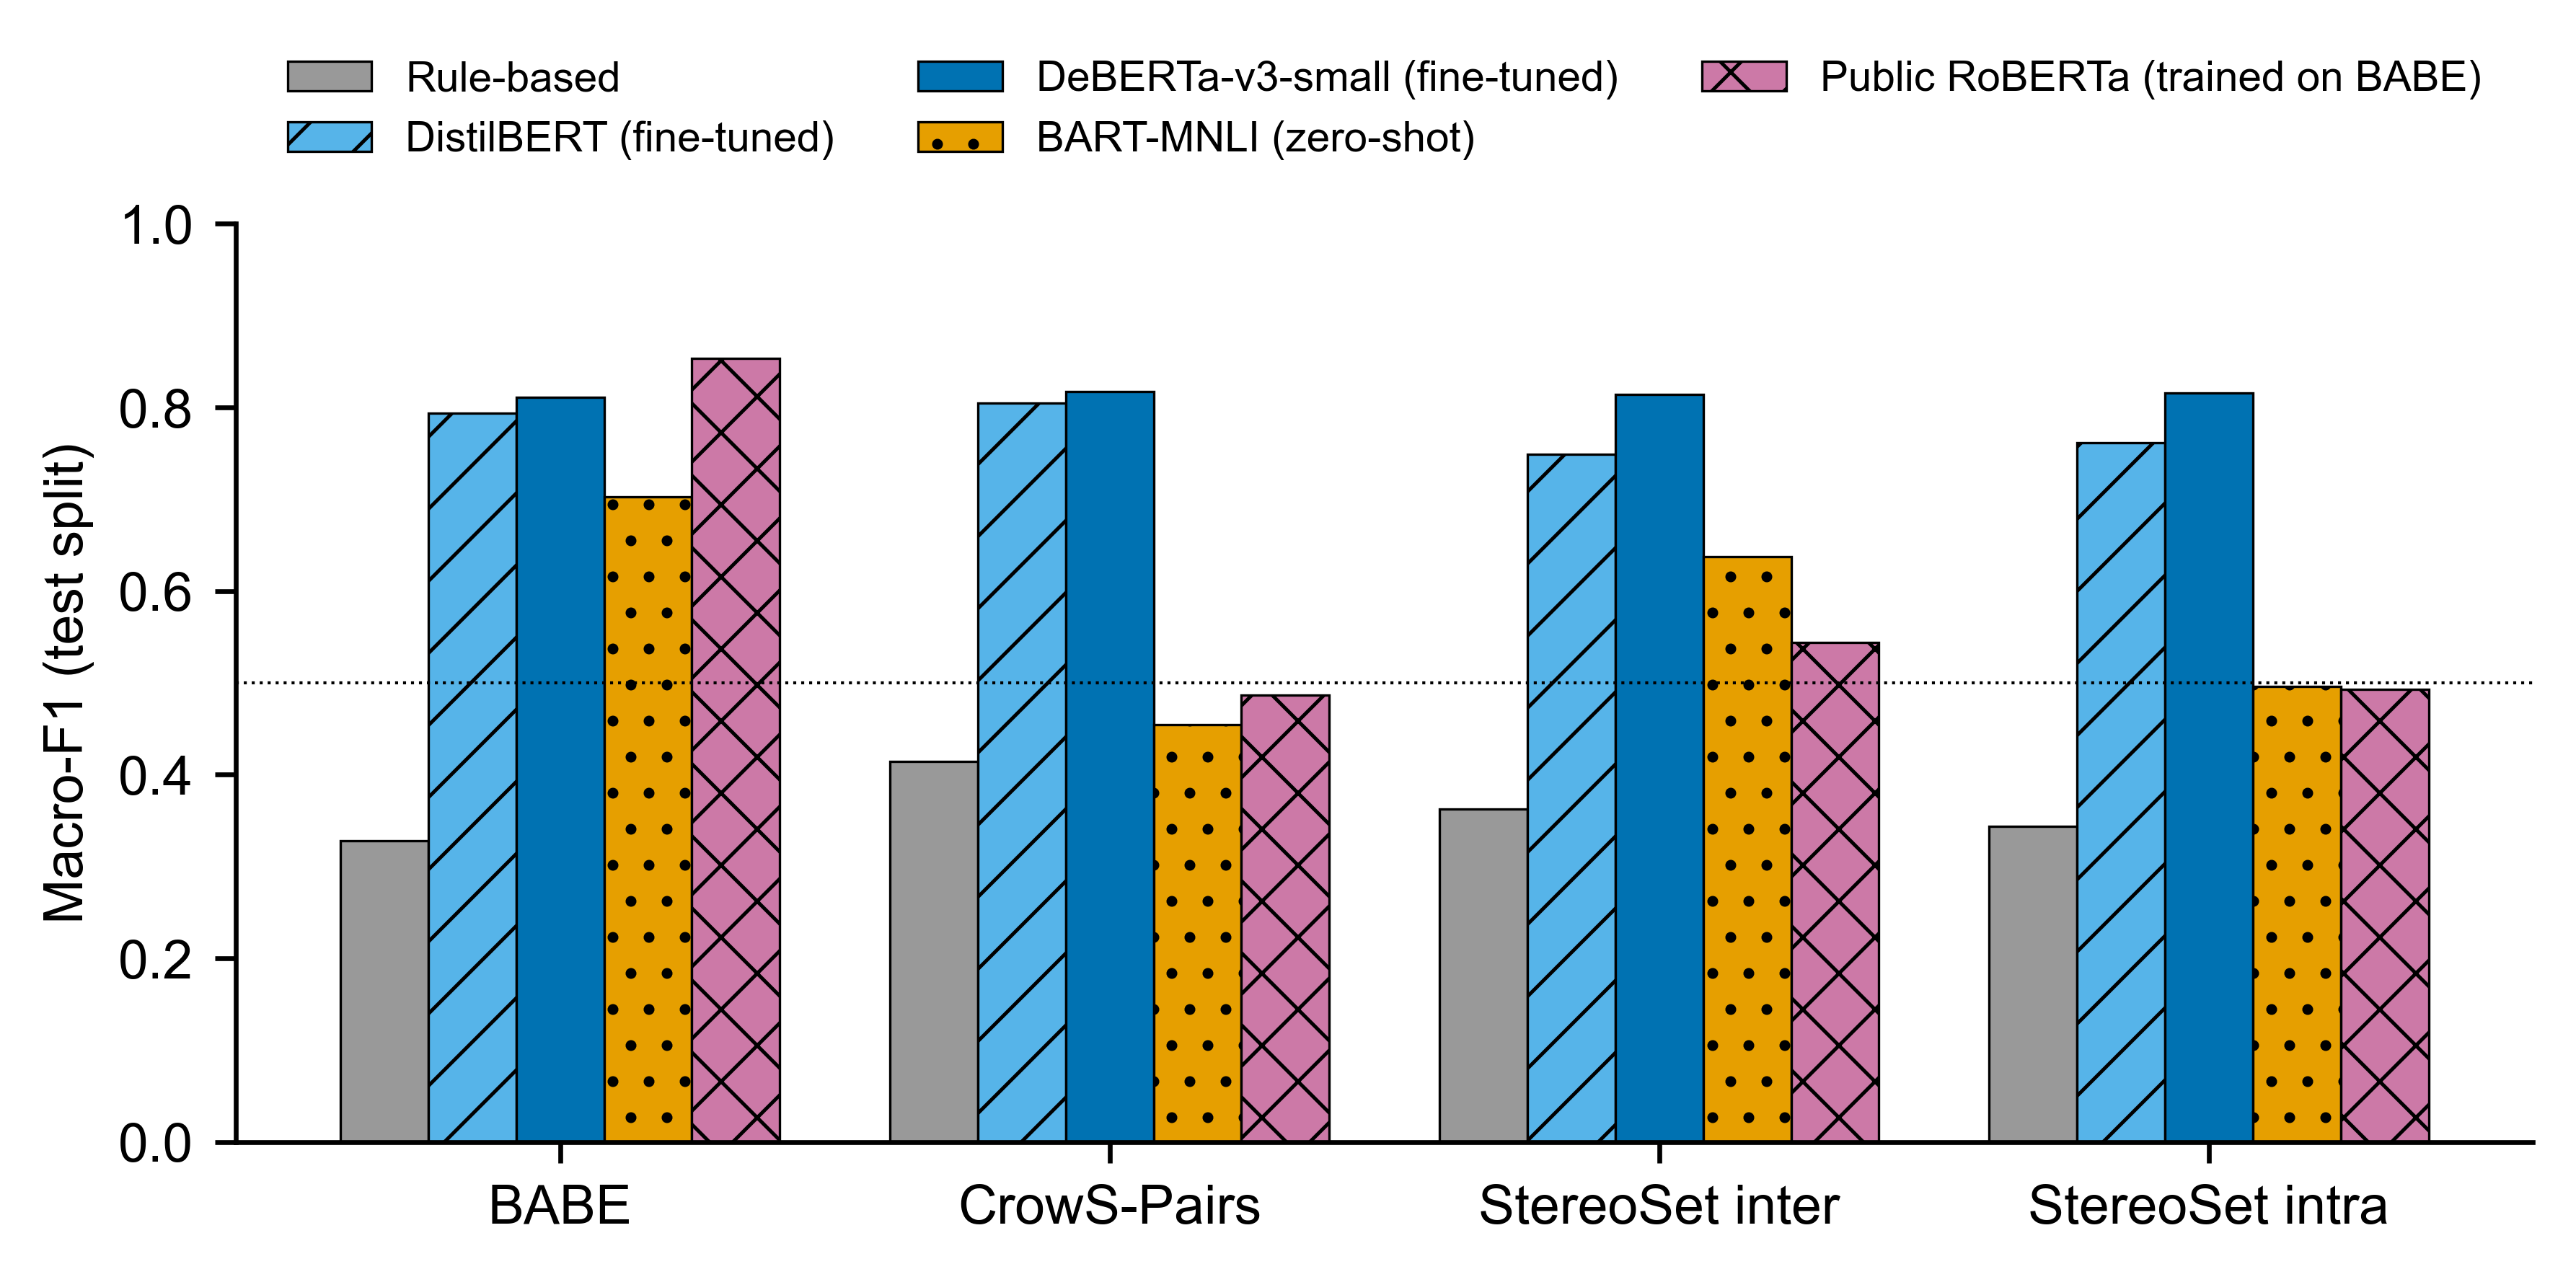
\includegraphics[width=0.95\textwidth]{figures/detector_f1.png}
\caption{Macro-F1 of each detector by data source on the test split. The dotted line marks 0.5.}
\label{fig:detf1}
\end{figure}

High benchmark accuracy did not mean few false alarms on everyday text. The fine-tuned detectors flagged 39.6\% and
37.6\% (DeBERTa) and 44.1\% and 42.8\% (DistilBERT) of the neutral WinoBias sentences. On minimal pairs, DeBERTa
preferred the more stereotypical CrowS-Pairs sentence in 90.1\% of pairs. Calibration errors of about 0.12 for the
fine-tuned models mean their scores should not be read as probabilities.

\section{Rewriting: Bias Reduction Against Preservation}
Table~\ref{tab:rew} and Figure~\ref{fig:biasfact} compare the rewriters on the 276 mitigation inputs. Qwen2.5 reduced
the mean bias score the most (0.087) but lost at least one extracted fact in 41.7\% of its rewrites and changed 98.5\%
of the neutral inputs that needed no change. The rule rewriter achieved a similar reduction (0.074) with a fact failure
rate of 1.8\%, because it only substitutes terms. FLAN-T5 changed only 31.2\% of inputs and reduced bias by 0.018: it
mostly copied its input, a capability limit we report rather than hide.

\begin{longtable}{|L{2.8cm}|L{2.3cm}|c|c|c|c|c|L{1.6cm}|}
\caption{Rewriters on the Mitigation Set (276 Inputs; 211 Biased, 65 Neutral)}\label{tab:rew}\\
\hline
\textbf{Rewriter} & \textbf{Bias reduction [95\% CI]} & \textbf{Changed} & \textbf{Sim.} & \textbf{Entail.} &
\textbf{Fact ret.} & \textbf{Fact fail.} & \textbf{Unnec. change}\\ \hline\endfirsthead
\hline \textbf{Rewriter} & \textbf{Bias reduction [95\% CI]} & \textbf{Changed} & \textbf{Sim.} & \textbf{Entail.} &
\textbf{Fact ret.} & \textbf{Fact fail.} & \textbf{Unnec. change}\\ \hline\endhead
Rule rewriter & 0.074 [0.056, 0.092] & 27.5\% & 0.899 & 0.286 & 0.994 & 1.8\% & 0.0\%\\ \hline
FLAN-T5-base & 0.018 [0.008, 0.031] & 31.2\% & 0.901 & 0.359 & 0.960 & 9.4\% & 20.0\%\\ \hline
Qwen2.5-0.5B-Instruct & 0.087 [0.064, 0.110] & 99.3\% & 0.828 & 0.464 & 0.801 & 41.7\% & 98.5\%\\ \hline
No change (reference) & 0.000 & 0.0\% & -- & -- & 1.000 & 0.0\% & 0.0\%\\ \hline
\end{longtable}

\begin{figure}[H]
\centering
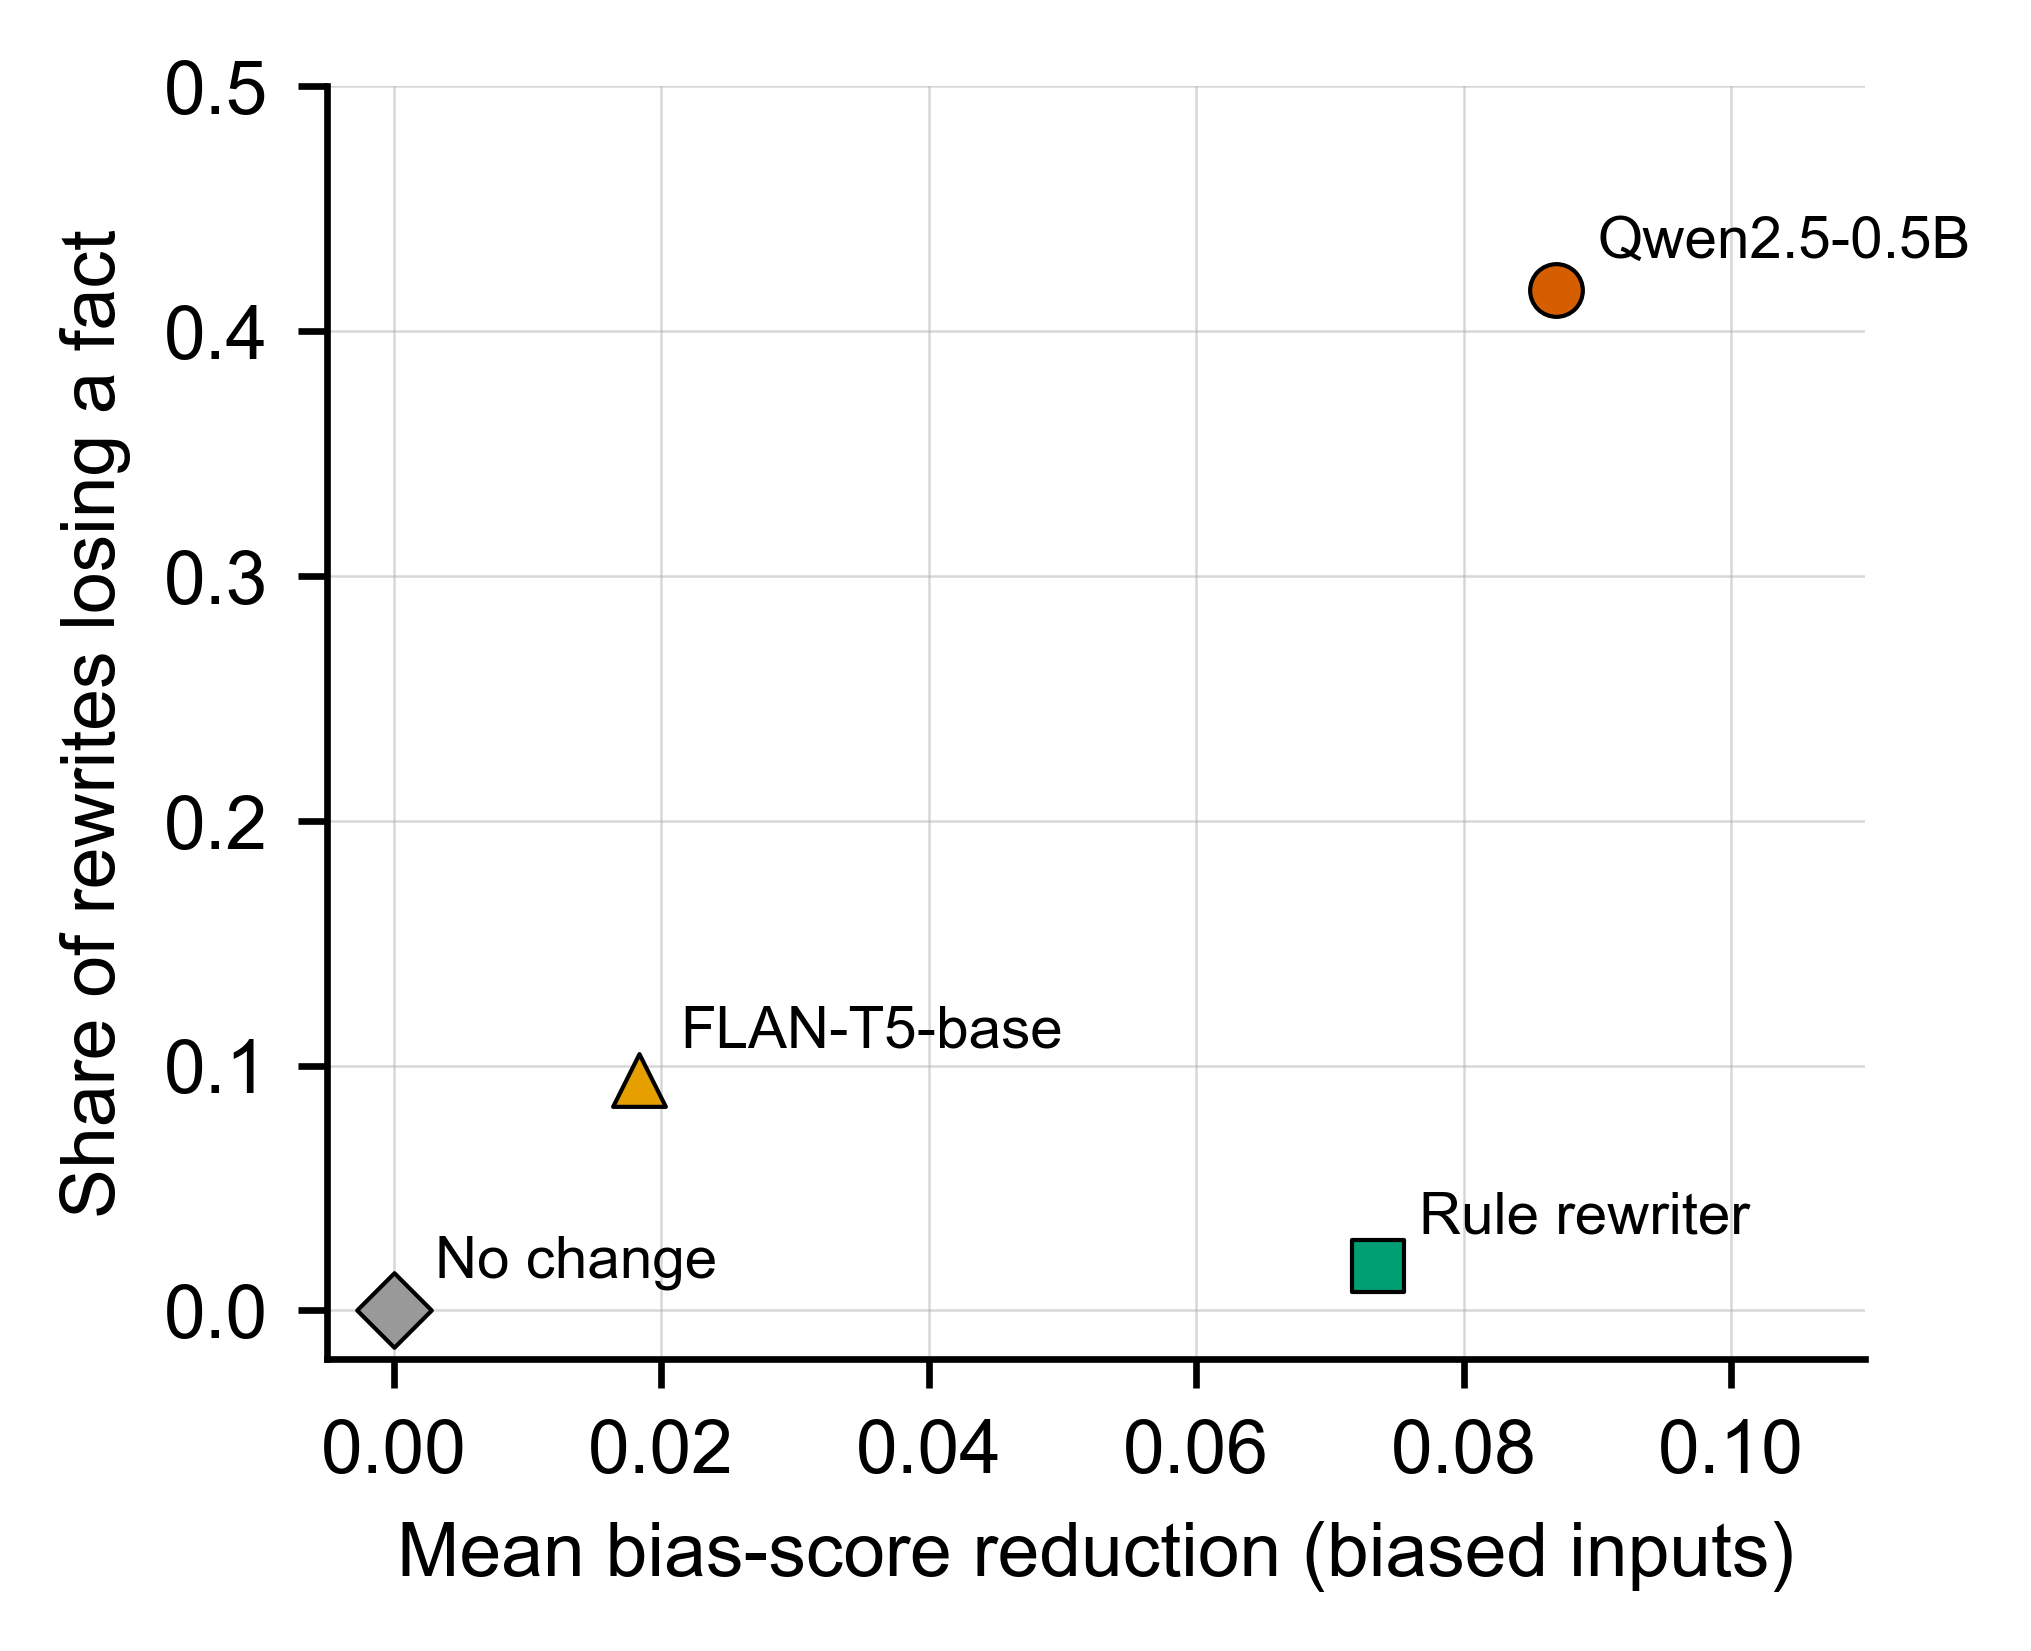
\includegraphics[width=0.7\textwidth]{figures/bias_vs_factloss.png}
\caption{Bias reduction against fact loss for each rewriter on the mitigation set.}
\label{fig:biasfact}
\end{figure}

Table~\ref{tab:real} applies the selection policies to these real rewrites. The Gate accepted no rewrite that lost a
fact or was contradicted by the NLI model, against 25.4\% and 8.3\% for lowest-bias selection, and it made no
unnecessary changes. The cost was 47.5\% of inputs deferred to a person and 26.5\% of biased inputs left unchanged,
which matches the detection rate: the detectors flagged only 73.5\% of the biased inputs. Of 124 inputs retried with the
strict prompt, only 3 were accepted after retry.

\begin{longtable}{|L{3.6cm}|c|c|c|c|c|L{1.8cm}|}
\caption{Selection Policies on Real Rewrites (276 Inputs)}\label{tab:real}\\
\hline
\textbf{Policy} & \textbf{Fact loss} & \textbf{Contradiction} & \textbf{Unnec. change} & \textbf{Bias red.} &
\textbf{Deferred} & \textbf{Biased left unchanged}\\ \hline\endfirsthead
\hline \textbf{Policy} & \textbf{Fact loss} & \textbf{Contradiction} & \textbf{Unnec. change} & \textbf{Bias red.} &
\textbf{Deferred} & \textbf{Biased left unchanged}\\ \hline\endhead
Rule Gate & 0.0\% & 0.0\% & 0.0\% & 0.121 & 47.5\% & 26.5\%\\ \hline
Rule Gate + strict retry & 0.0\% & 0.0\% & 1.5\% & 0.128 & 46.4\% & 26.5\%\\ \hline
Lowest bias score & 25.4\% & 8.3\% & 56.9\% & 0.152 & 0.0\% & 15.2\%\\ \hline
Highest similarity & 29.7\% & 6.5\% & 98.5\% & 0.088 & 0.0\% & 0.0\%\\ \hline
Always first model (FLAN-T5) & 9.4\% & 0.7\% & 20.0\% & 0.018 & 0.0\% & 65.4\%\\ \hline
Random (mean of 5 seeds) & 36.1\% & 7.8\% & 98.5\% & 0.089 & 0.0\% & 0.0\%\\ \hline
\end{longtable}

\section{The Reliability Gate on Known Correct Decisions}
Table~\ref{tab:ctrl} and Figure~\ref{fig:policy} report input-level selection on the 204 test inputs of the controlled
set. Choosing the least-biased candidate was almost always wrong: it chose a damaging rewrite for 196 of 204 inputs
(96.1\%). Highest-similarity selection made more acceptable choices than the rule Gate (59.3\% against 42.6\%), but every
one of its errors was a damaging rewrite and it changed every neutral input. The validation-tuned rule Gate's
harmful-choice rate was 33.8\%, but all of these cases were biased originals kept unchanged; it never chose a damaging
rewrite. It deferred 23.5\% of inputs and made no unnecessary changes. The learned decision tree was the most accurate
policy (76.0\% acceptable choices, 4.9\% deferred), but it chose a damaging rewrite 27 times and changed 26.1\% of
neutral inputs.

\begin{longtable}{|L{3.4cm}|L{2.2cm}|L{2.2cm}|c|c|c|c|}
\caption{Input-Level Selection on the Controlled Test Split (204 Inputs)}\label{tab:ctrl}\\
\hline
\textbf{Policy} & \textbf{Acceptable [95\% CI]} & \textbf{Harmful [95\% CI]} & \textbf{Kept biased} & \textbf{Damaging} &
\textbf{Deferred} & \textbf{Unnec.}\\ \hline\endfirsthead
\hline \textbf{Policy} & \textbf{Acceptable [95\% CI]} & \textbf{Harmful [95\% CI]} & \textbf{Kept biased} &
\textbf{Damaging} & \textbf{Deferred} & \textbf{Unnec.}\\ \hline\endhead
Lowest bias score & 0.015 [0.000, 0.034] & 0.985 [0.966, 1.000] & 0.025 & 0.961 & 0.000 & 0.957\\ \hline
Highest similarity & 0.593 [0.520, 0.662] & 0.407 [0.338, 0.480] & 0.000 & 0.407 & 0.000 & 1.000\\ \hline
Keep original & 0.338 [0.279, 0.402] & 0.662 [0.598, 0.721] & 0.662 & 0.000 & 0.000 & 0.000\\ \hline
LLM-as-judge (Qwen2.5) & 0.235 [0.181, 0.294] & 0.319 [0.260, 0.377] & 0.000 & 0.319 & 0.446 & 0.899\\ \hline
Rule Gate (default) & 0.324 [0.265, 0.387] & 0.338 [0.279, 0.407] & 0.338 & 0.000 & 0.338 & 0.000\\ \hline
\textbf{Rule Gate (tuned)} & 0.426 [0.363, 0.490] & 0.338 [0.279, 0.407] & 0.338 & \textbf{0.000} & 0.235 & \textbf{0.000}\\ \hline
Learned gate (logistic) & 0.603 [0.534, 0.667] & 0.216 [0.162, 0.275] & 0.000 & 0.216 & 0.181 & 0.464\\ \hline
Learned gate (tree) & 0.760 [0.701, 0.819] & 0.191 [0.142, 0.250] & 0.059 & 0.132 & 0.049 & 0.261\\ \hline
Random (mean of 5 seeds) & 0.130 & 0.870 & -- & -- & 0.000 & 1.000\\ \hline
\end{longtable}

\begin{figure}[H]
\centering
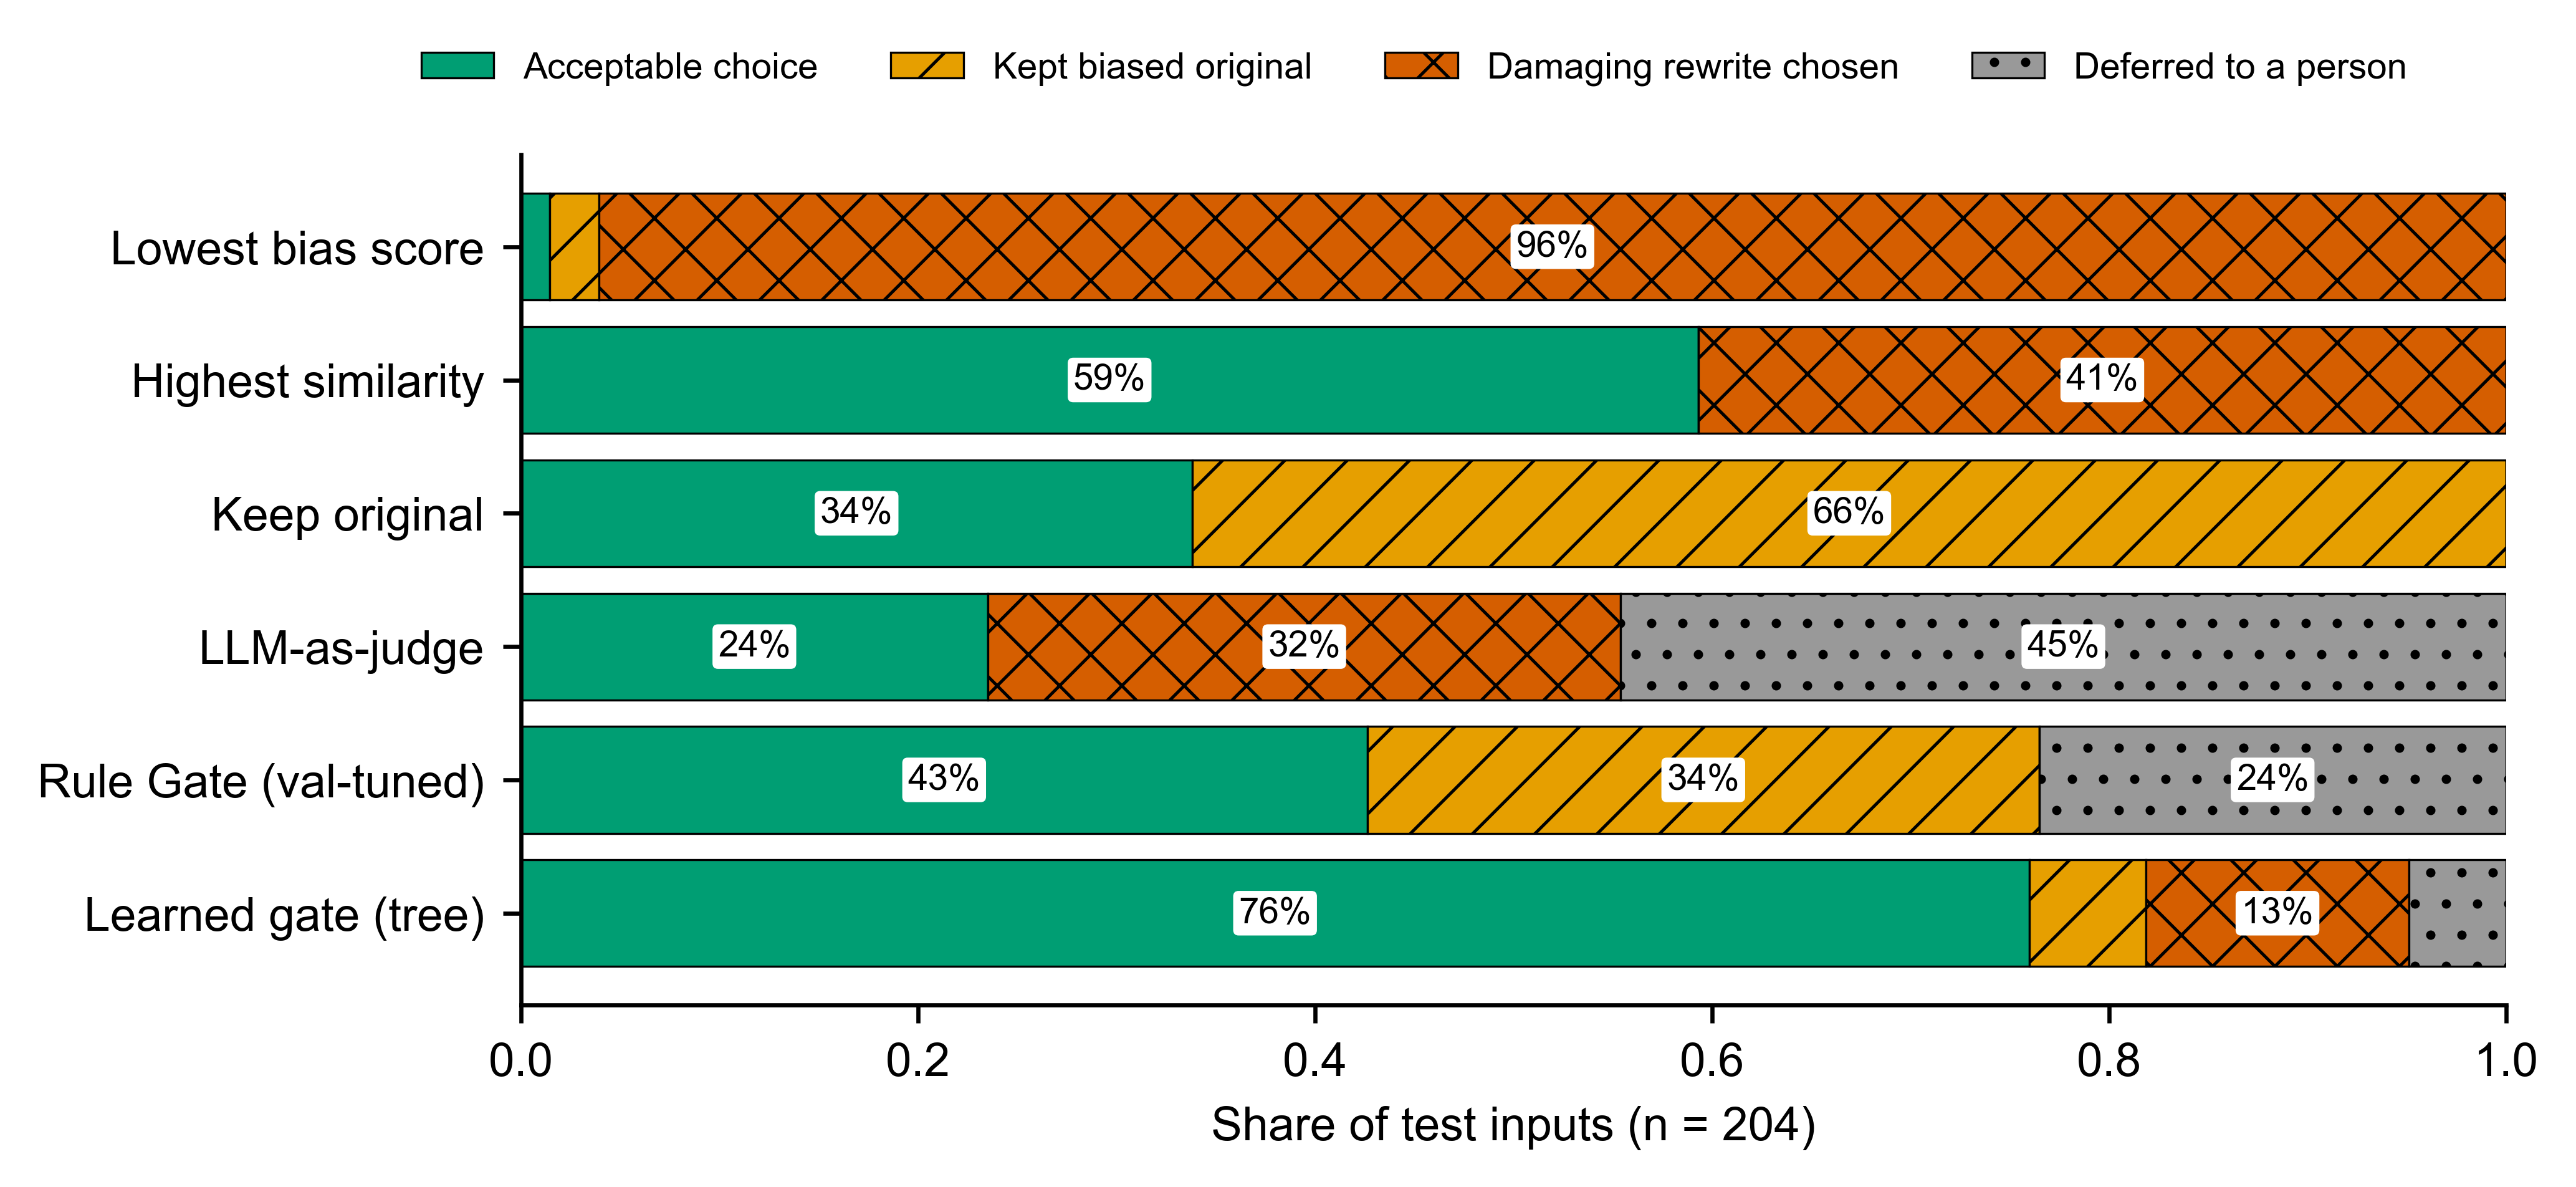
\includegraphics[width=0.98\textwidth]{figures/policy_outcomes.png}
\caption{Outcome of each selection policy on the 204 test inputs of the controlled set.}
\label{fig:policy}
\end{figure}

At the candidate level the tuned rule Gate reached a three-class macro-F1 of 0.665 with an unsafe-accept rate of 7.1\%.
Its unsafe accepts were all unchanged biased originals accepted because the detectors did not judge the input biased;
none was a corrupted rewrite. When the gold input label was supplied instead of the detectors' judgement, the
unsafe-accept rate fell to 0.3\% and macro-F1 rose to 0.864. The Gate's remaining failures are therefore inherited mainly
from detection, not from its preservation checks.

\section{Which Signals Matter}
Table~\ref{tab:abl} removes one signal group at a time from the tuned rule Gate. Removing the bias-reduction check raised
the unsafe-accept rate by 6.2 percentage points and removing entailment by 5.6; removing fact retention had a small but
non-zero effect (0.6 points), largely because entailment also catches most planted corruptions. Detector agreement,
uncertainty and fluency had no measurable effect on this set, which we report as a negative result.

\begin{longtable}{|L{3.4cm}|c|L{3.4cm}|c|L{3.4cm}|}
\caption{Ablations of the Tuned Rule Gate on the Controlled Test Candidates ($n$ = 1,218)}\label{tab:abl}\\
\hline
\textbf{Signal removed} & \textbf{Unsafe accept} & \textbf{$\Delta$ unsafe accept [95\% CI]} & \textbf{Macro-F1} &
\textbf{$\Delta$ accuracy [95\% CI]}\\ \hline\endfirsthead
\hline \textbf{Signal removed} & \textbf{Unsafe accept} & \textbf{$\Delta$ unsafe accept [95\% CI]} & \textbf{Macro-F1}
& \textbf{$\Delta$ accuracy [95\% CI]}\\ \hline\endhead
None (full Gate) & 0.071 & -- & 0.665 & --\\ \hline
Bias reduction & 0.133 & +0.062 [+0.048, +0.076] & 0.461 & $-$0.044 [$-$0.059, $-$0.031]\\ \hline
Entailment & 0.127 & +0.056 [+0.042, +0.072] & 0.632 & $-$0.047 [$-$0.060, $-$0.034]\\ \hline
Fact retention & 0.077 & +0.006 [+0.002, +0.011] & 0.665 & $-$0.008 [$-$0.016, +0.000]\\ \hline
Semantic similarity & 0.074 & +0.003 [+0.000, +0.007] & 0.664 & $-$0.002 [$-$0.006, +0.000]\\ \hline
Detector agreement & 0.071 & +0.000 [+0.000, +0.000] & 0.665 & +0.000 [+0.000, +0.000]\\ \hline
Uncertainty & 0.071 & +0.000 [+0.000, +0.000] & 0.665 & +0.000 [+0.000, +0.000]\\ \hline
Fluency & 0.071 & +0.000 [+0.000, +0.000] & 0.669 & +0.000 [$-$0.004, +0.004]\\ \hline
\end{longtable}

\section{Image Captions}
On 80 COCO validation images (60 showing people), Florence-2 captions were as well aligned with the images as the human
reference captions (CLIP similarity 0.306 against 0.304 for references and 0.281 for BLIP). Gendered terms appeared in
53.3\% (BLIP) and 60.0\% (Florence-2) of captions of images with people, against 73.3\% in the human references. No
caption contained an attribute that pixels cannot normally verify. The text detectors flagged 47.5\% and 68.8\% of
captions as biased; given the false-alarm rates in Section 5.1 we do not read these as bias rates.

\section{Working Application}
The dashboard has twelve pages grouped into a workflow section (Home, FairLens Review, Text Analysis, Mitigation,
Reliability Gate, Image Analysis), a research section (Benchmarks, Model Comparison, Error Analysis, Experiments and
Exports) and supporting pages (Use Cases, About). The FairLens Review page (Figure~\ref{fig:review}) guides a user
through a six-step check of a job advertisement: input, flagged phrases, rewrites with a diff view, fact checks, the
Gate's verdict with reason codes, and export. Snapshots of every main page, including a live end-to-end demo, are given
in Appendix A.

\begin{figure}[H]
\centering
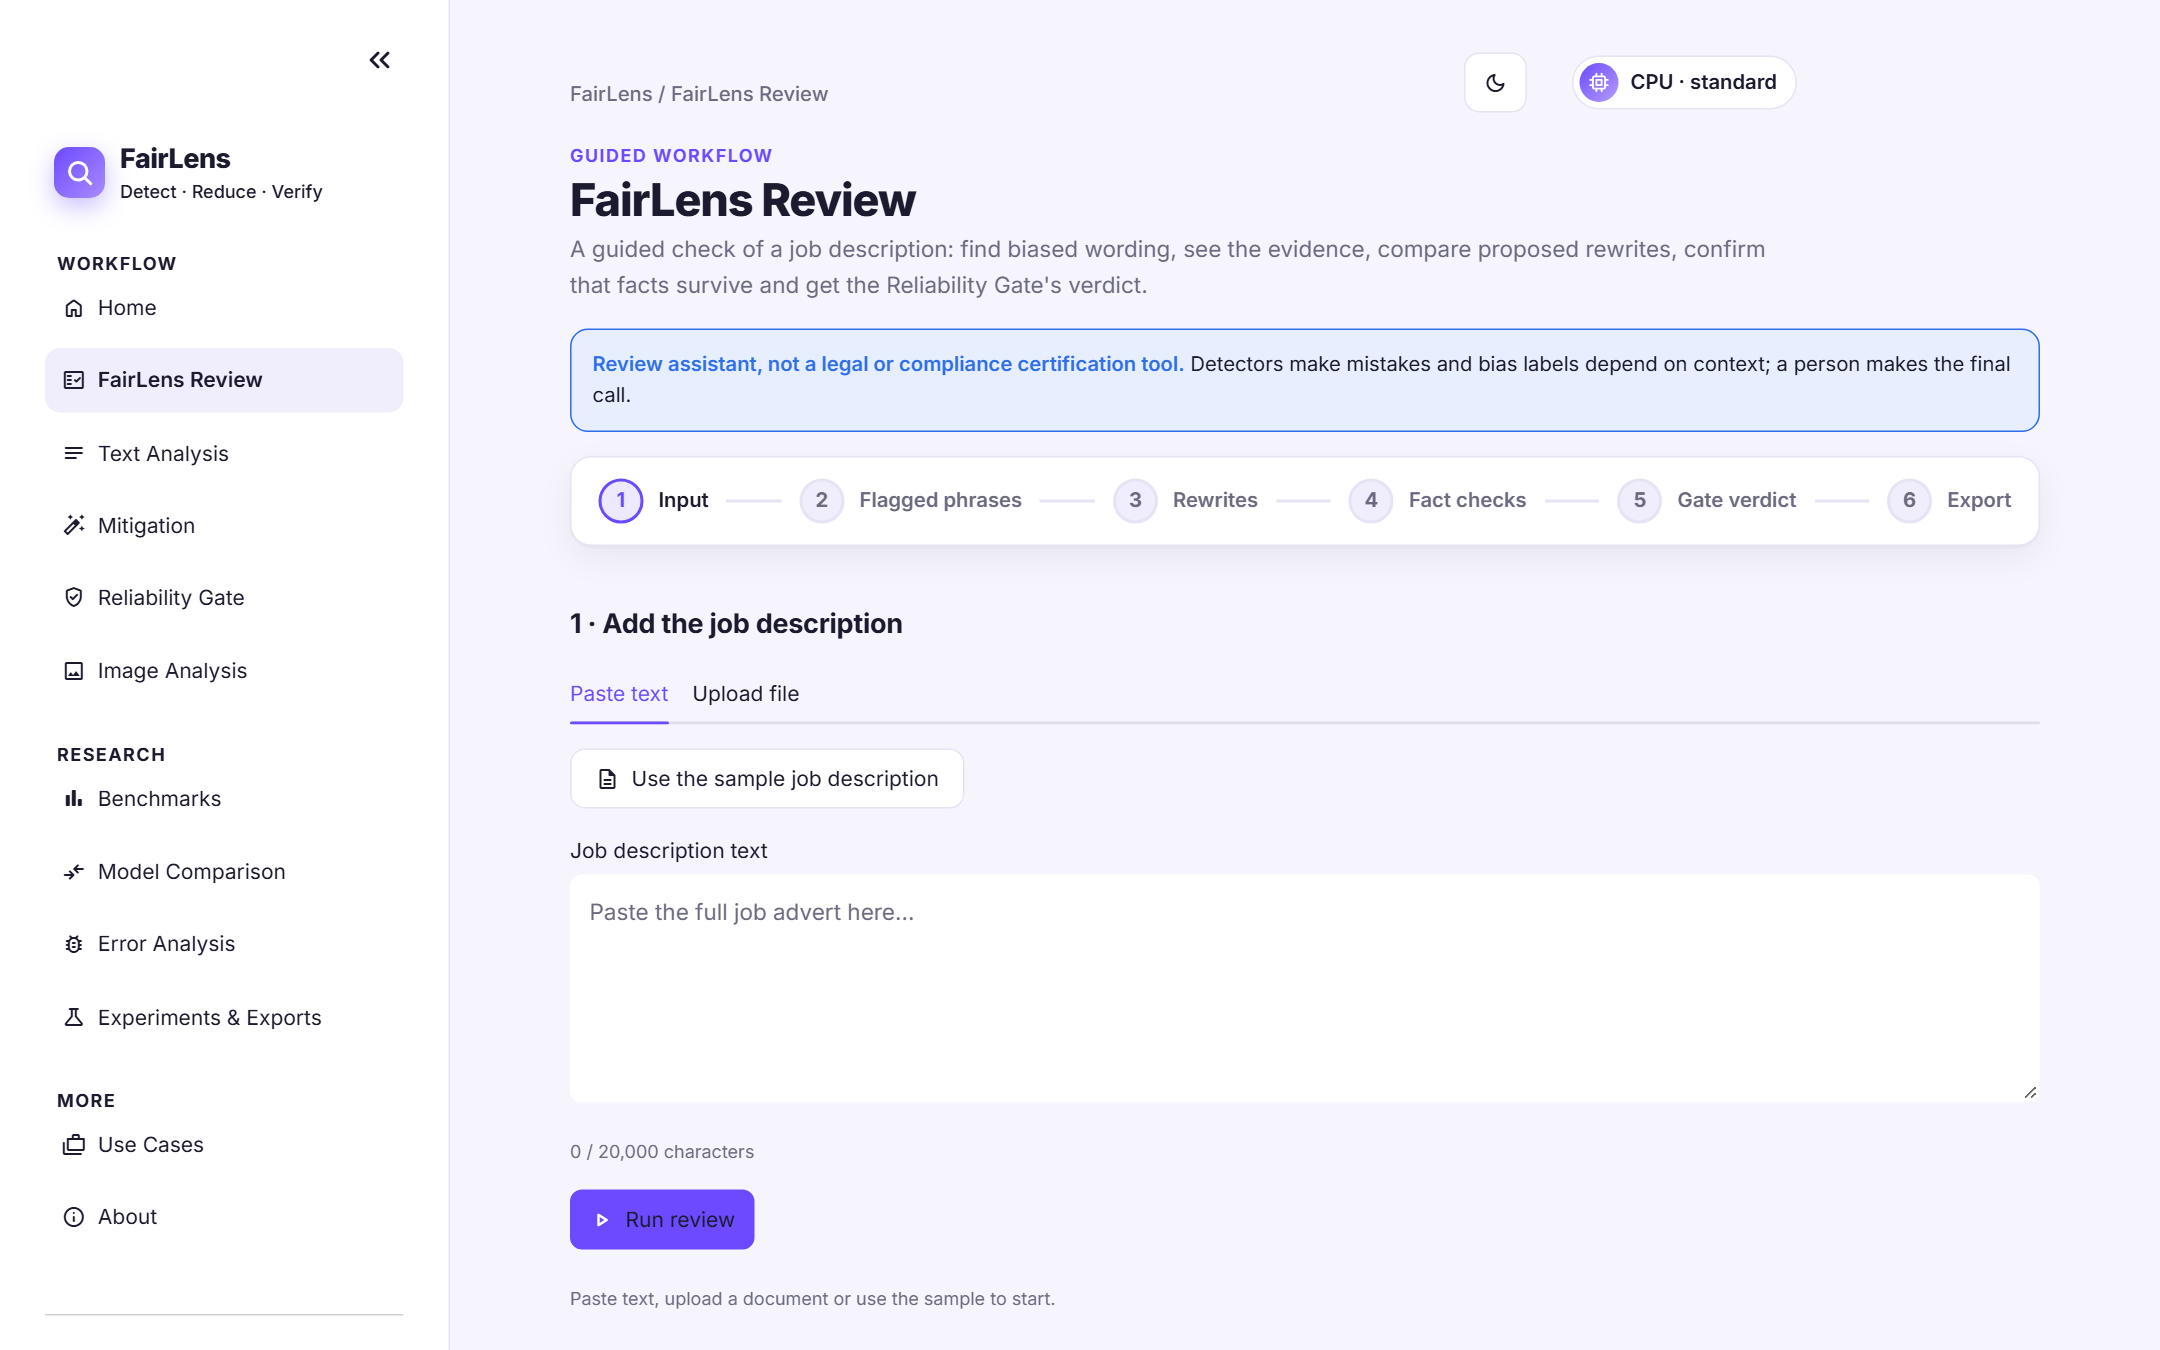
\includegraphics[width=0.95\textwidth]{figures/review_page.png}
\caption{The FairLens Review page: a guided six-step check of a job description.}
\label{fig:review}
\end{figure}

\section{Live Demonstration}
To show the complete pipeline working end to end, a new job advertisement was entered into the running application
(standard profile, CPU):

\begin{quote}
``We are looking for a young, energetic waitress to join our Bengaluru cafe. She must be available 6 days a week and
have 2 years of experience.''
\end{quote}

\textbf{Step 1: Detection.} All four detectors judged the text biased (Table~\ref{tab:demo_det}); the overall score
was 0.72. The rule detector explained its flags as a gender-marked term (``waitress'') and age-coded wording
(``young''), and highlighted the phrases in the text (Figure~\ref{fig:demo_det}).

\begin{longtable}{|L{4cm}|c|L{7.5cm}|}
\caption{Live Demo: Detector Scores for the Demo Advertisement}\label{tab:demo_det}\\
\hline
\textbf{Detector} & \textbf{Score} & \textbf{Explanation shown}\\ \hline\endfirsthead
\hline \textbf{Detector} & \textbf{Score} & \textbf{Explanation shown}\\ \hline\endhead
DistilBERT (fine-tuned) & 0.51 & Biased\\ \hline
DeBERTa-v3-small (fine-tuned) & 0.86 & Biased\\ \hline
BART-MNLI (zero-shot) & 0.98 & Biased\\ \hline
Rule-based & 0.55 & Gender: ``waitress''; Age: ``young''\\ \hline
\textbf{Overall} & \textbf{0.72} & High bias\\ \hline
\end{longtable}

\begin{figure}[H]
\centering
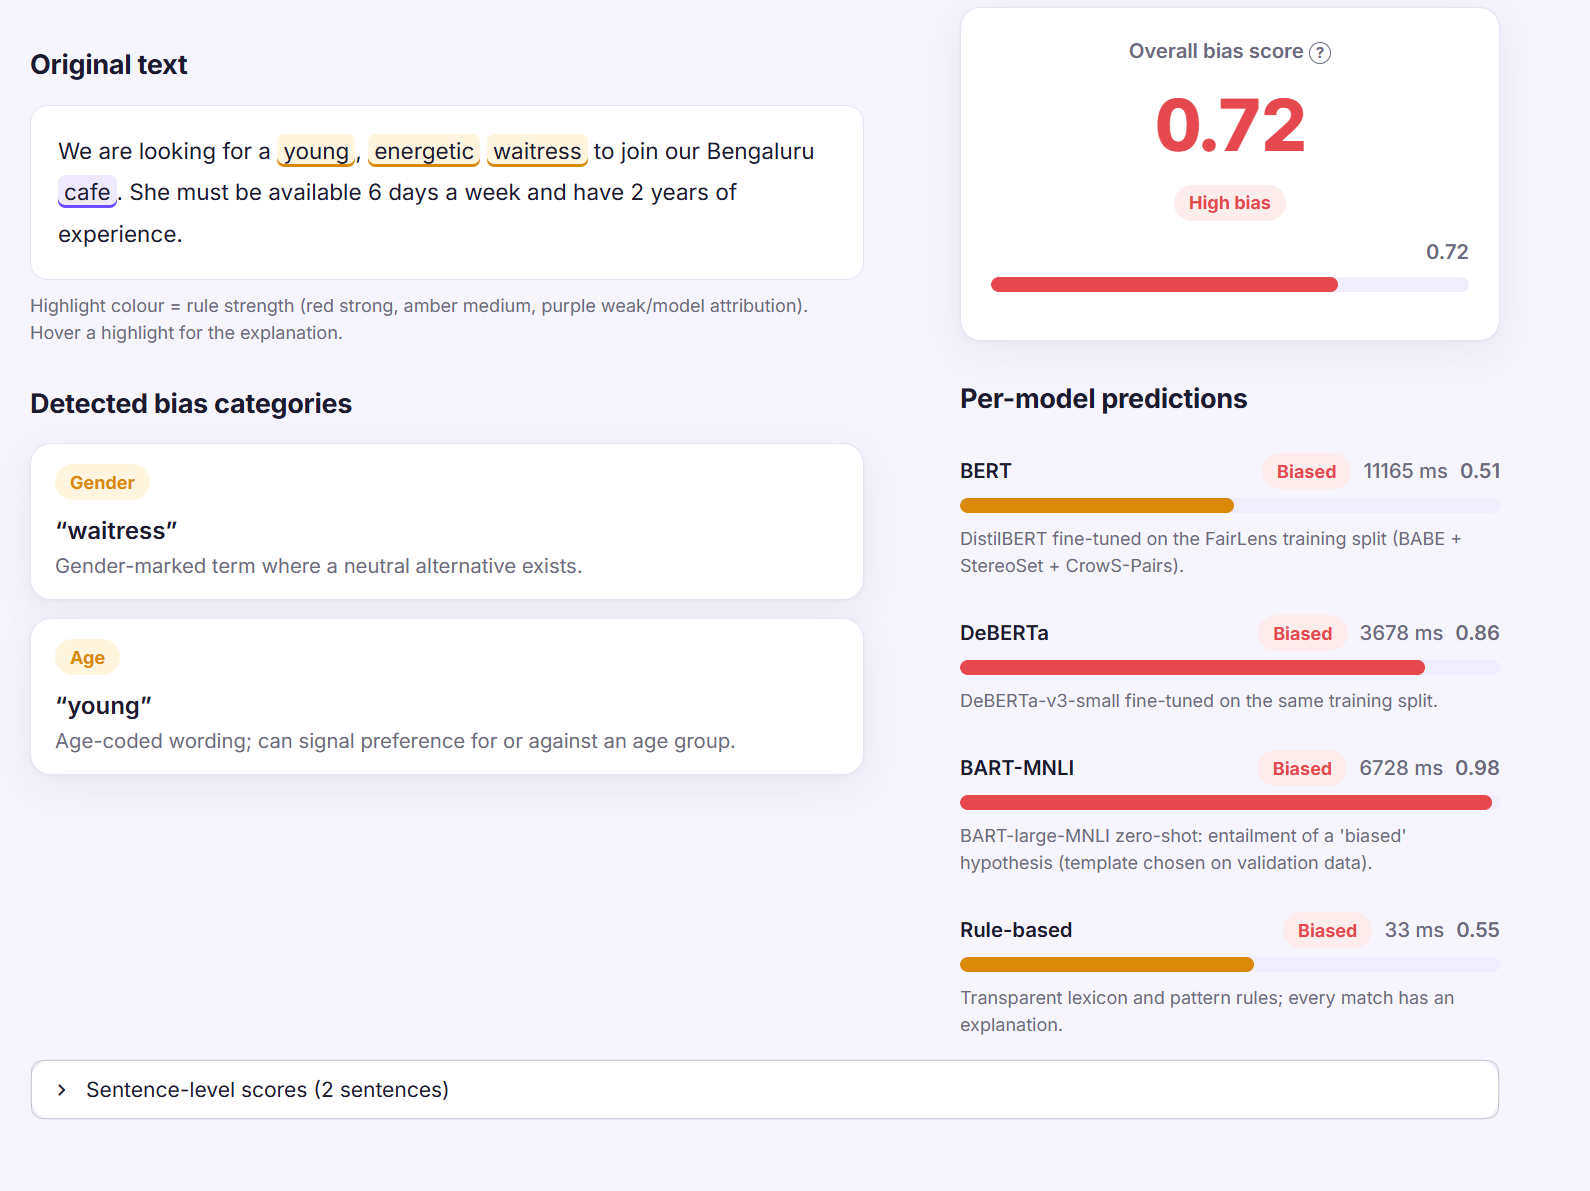
\includegraphics[width=0.85\textwidth]{figures/demo_detection.png}
\caption{Live demo, step 1: highlighted phrases, bias categories and per-detector scores}
\label{fig:demo_det}
\end{figure}

\textbf{Steps 2--3: Mitigation and Reliability Gate.} Table~\ref{tab:demo_gate} and Figure~\ref{fig:demo_mit} show
the three rewrites and the Gate's verdicts.

\begin{longtable}{|L{2.1cm}|L{5.6cm}|L{1.5cm}|c|c|c|}
\caption{Live Demo: Rewrites and Reliability Gate Verdicts}\label{tab:demo_gate}\\
\hline
\textbf{Version} & \textbf{Text} & \textbf{Verdict} & \textbf{Bias score} & \textbf{Sim.} & \textbf{Facts}\\ \hline\endfirsthead
\hline \textbf{Version} & \textbf{Text} & \textbf{Verdict} & \textbf{Bias score} & \textbf{Sim.} & \textbf{Facts}\\ \hline\endhead
Original & (input above) & Retry & 0.561 & 1.000 & 1.000\\ \hline
Rule-based & ``We are looking for an energetic server to join our Bengaluru cafe. She must be available 6 days a week and
have 2 years of experience.'' & \textbf{Accept} & 0.300 & 0.772 & 1.000\\ \hline
FLAN-T5 & Unchanged copy of the input & Retry & 0.561 & 1.000 & 1.000\\ \hline
Qwen2.5 & ``We're seeking an enthusiastic waitress to join our bustling Bengaluru caf\'e. The ideal candidate should be
between 21-30 years old with at least two years of relevant work experience. They must be available every day from
Monday to Friday.'' & Reject & 0.558 & 0.892 & 0.667\\ \hline
\end{longtable}

\begin{figure}[H]
\centering
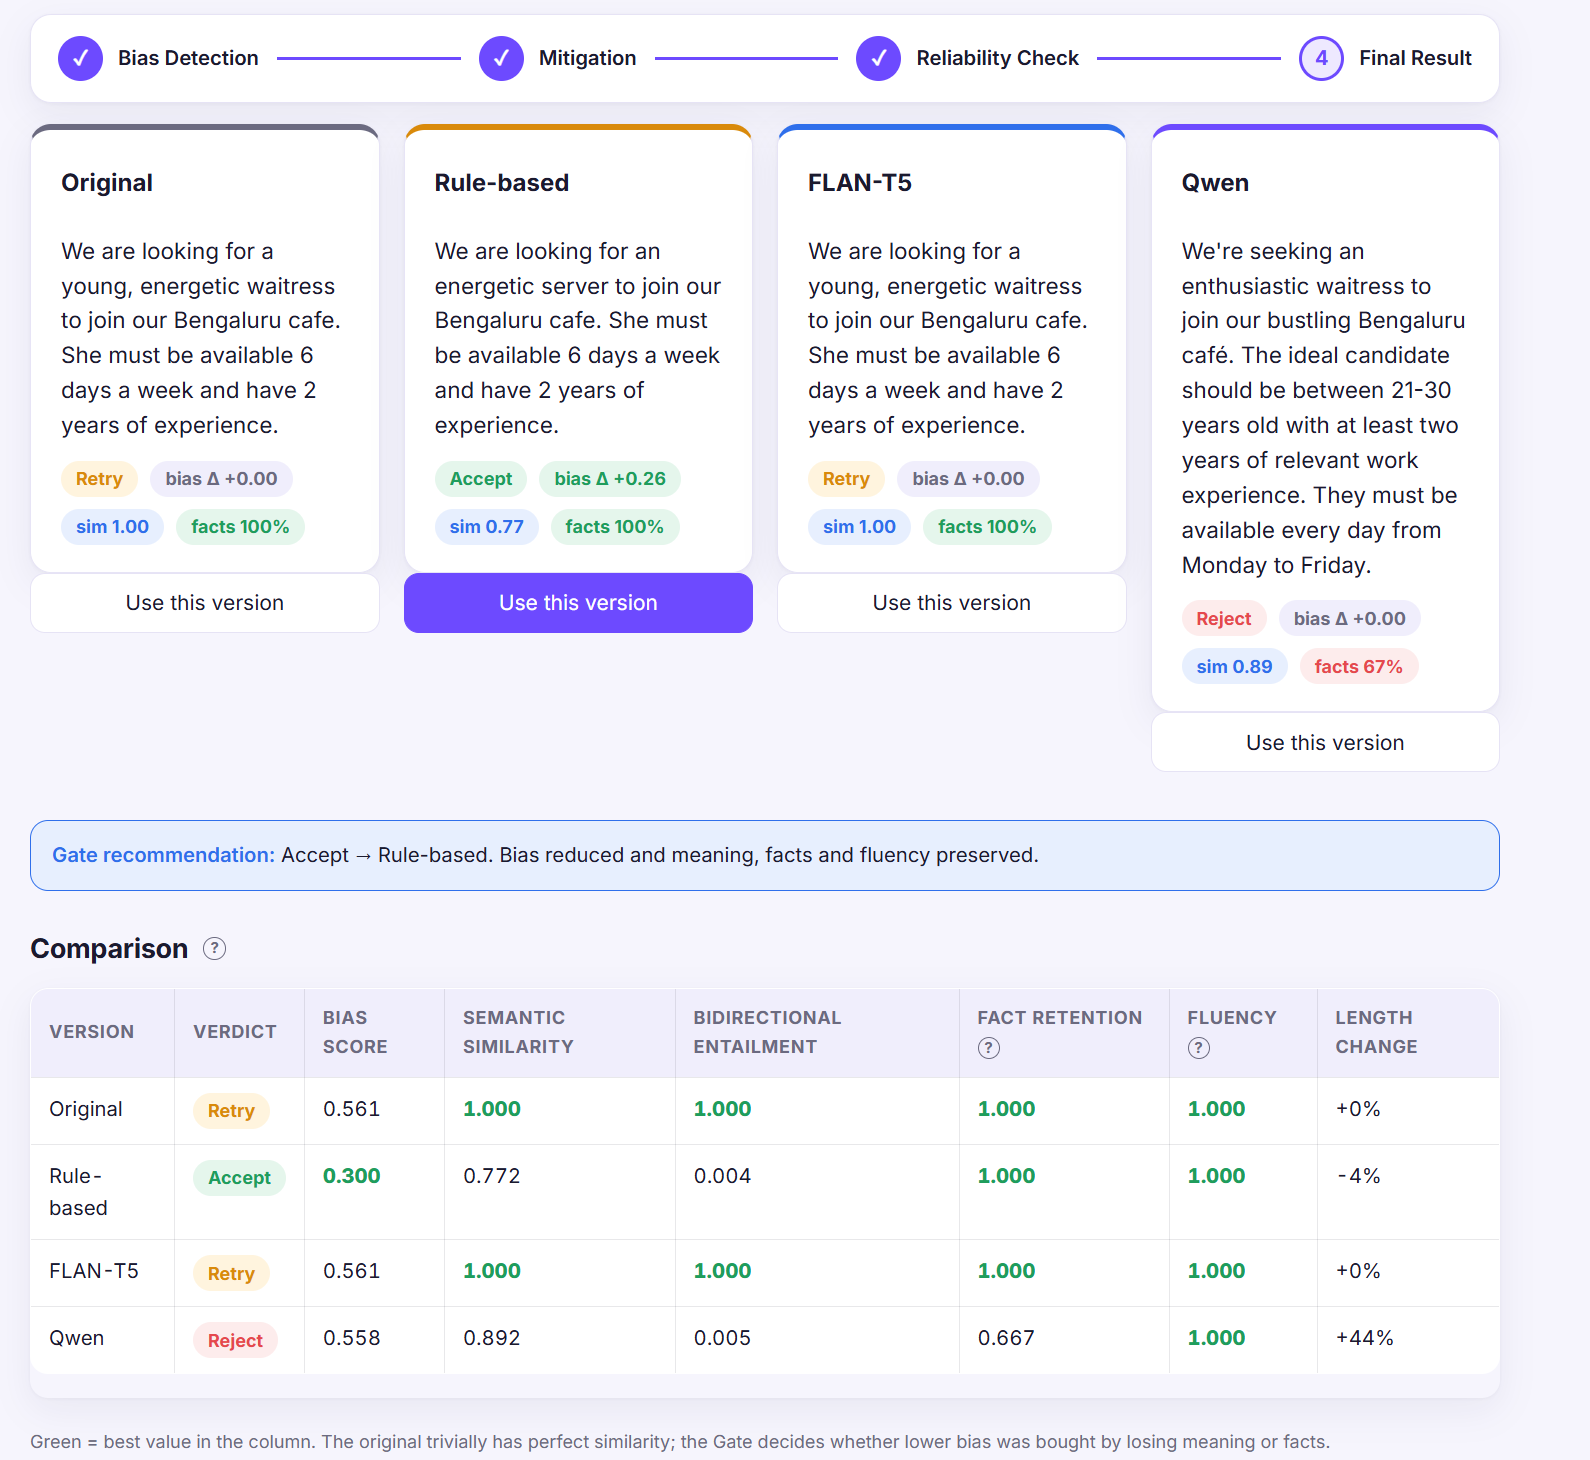
\includegraphics[width=0.95\textwidth]{figures/demo_mitigation_core.png}
\caption{Live demo, steps 2--3: the three rewrites with their Gate verdicts and the comparison table}
\label{fig:demo_mit}
\end{figure}

The Gate accepted the rule-based rewrite with the reason code ALL\_CHECKS\_PASSED: its bias score fell from 0.561 to
0.300, every extracted fact survived, semantic similarity was 0.77 (threshold 0.60) and forward entailment 0.98
(threshold 0.70). FLAN-T5 copied its input and was sent for a retry. Qwen2.5 produced the most fluent advertisement, but
it \emph{added} an age range (``between 21-30 years old''), changed ``6 days a week'' to ``every day from Monday to
Friday'' and kept ``waitress''; with fact retention 0.67 the Gate rejected it. This single example reproduces the
project's central finding: the most fluent LLM rewrite introduced new, more discriminatory content and changed a fact,
and only the preservation checks caught it. The accepted rewrite still contains the pronoun ``She'', which the rule
lexicon does not change; because the detectors no longer flagged the sentence, the Gate did not request a further
rewrite. This is an illustrative run, not a benchmark result.


\section{Verification}
The code base has an automated test suite covering ingestion of every supported format and its edge cases,
segmentation, the fact extractor and Gate rules, metrics, run tracking, the pipeline end to end, and the dashboard
pages, including a test that no page displays a metric that is not read from a run file. After the final re-split of
the controlled set, 245 of 246 tests passed in the project environment on a Windows laptop; the remaining test, which
fits the learned gates, passed under the Anaconda interpreter, because the device's Application Control policy blocks a
compiled scikit-learn library in the project environment. A browser-driven test of the review flow passed all 54 checks
on the original development machine, and a continuous-integration workflow passed the test suite on Windows, macOS and
Linux. The script that builds the controlled set also checks that no source sentence appears in more than one split.

\section{Discussion}
\textbf{A bias score is not an acceptance criterion.} On the controlled set, lowest-bias selection chose a damaging
rewrite for 96.1\% of inputs; on real rewrites it accepted outputs that lost a fact a quarter of the time. The stronger
rewriter was the less faithful one. Mitigation work should report preservation measures and unnecessary-change rates
alongside bias reduction.

\textbf{Abstention moves work to people.} The Gate deferred 23.5\% of controlled inputs and 47.5\% of real ones, and kept
the biased original for 33.8\% of controlled inputs. Deferral is only responsible where a qualified person will actually
review the case. Lowering the detection threshold would catch more bias but, given false-alarm rates near 40\% on
neutral WinoBias sentences, would also rewrite many authors' words for no reason. Better detection, not more rewriting
freedom, is the main route to fewer misses.

\textbf{Transparency has an accuracy cost.} The learned decision tree made more acceptable choices (76.0\% against
42.6\%) with fewer deferrals, but chose a damaging rewrite for 13.2\% of inputs, while the rule Gate never did and gives
reason codes an author can check and contest. In high-risk settings such as recruitment we consider this worth the lower
accuracy, but it is a value judgement deployers should make openly.

\textbf{What the tool should claim.} FairLens is a review assistant. It cannot certify that a text is unbiased;
presenting it as proof of compliance would be fairness-washing.

\section{Limitations}\label{sec:limits}
\begin{itemize}
\item The controlled gold set and reference rewrites were written by one author and its perturbations are synthetic, so
the high catch rates are partly by construction.
\item Mitigation quality was measured automatically; there is no human evaluation of the real rewrites yet.
\item Each experiment was run once, so confidence intervals reflect sampling of test items, not training seeds.
\item The controlled-set and Gate experiments were re-run on a different device (Windows, CPU) from the original
training and signal runs; they reuse the stored signals, so only the analysis environment differs.
\item All data are English, and the detectors were trained on news framing and stereotype sentences, not job
advertisements.
\item The rewriters are small (0.5 billion and 250 million parameters).
\item The BART-MNLI hypothesis template chosen on validation was not propagated to the Gate and mitigation runs.
\item The image experiment used 80 images and measures only caption wording.
\end{itemize}

% =====================================================================================
% CHAPTER 6
% =====================================================================================
\chapter{Conclusion and Future Work}\label{ch:conc}

\section{Conclusion}
FairLens is an automated framework that detects bias in text and image captions, proposes neutral rewrites and checks
each rewrite before it is accepted, in a laptop-scale application in which every number is traceable to a stored run.
Its evaluation shows that bias-mitigation rewrites should be accepted for what they keep as well as for what they
remove. On a controlled set with known answers, choosing the least-biased rewrite was almost always harmful, while a
transparent gate that checks facts and meaning never chose a damaging rewrite, at the price of deferring 23.5\% of inputs
and keeping the biased original for 33.8\% of inputs. A learned gate was more accurate but chose damaging rewrites more
often and was less explainable. All five objectives of Section 1.3 were met, with the limitations listed in
Section~\ref{sec:limits}.

\section{Future Work}
\begin{itemize}
\item A blinded human evaluation of real rewrites and of the Gate's decisions, with several annotators.
\item Repeated training runs with different seeds, and verification of all results on a second device.
\item A larger set of real job advertisements and other domain texts, with domain-specific definitions of the facts that
must be preserved.
\item A hybrid gate that keeps the rule Gate's hard preservation checks and reason codes but learns its thresholds,
with risk--coverage curves and threshold-sensitivity analysis.
\item Red-team tests in which real accepted rewrites are corrupted, to measure the Gate beyond synthetic perturbations.
\item Larger local rewriters and multilingual detectors, including Indian languages.
\end{itemize}

% =====================================================================================
% REFERENCES
% =====================================================================================
\clearpage
\addcontentsline{toc}{chapter}{References}
\renewcommand{\bibname}{References}
\begin{thebibliography}{99}
\bibitem{gaucher} D. Gaucher, J. Friesen, and A. C. Kay, ``Evidence that gendered wording in job advertisements exists and sustains gender inequality,'' \textit{J. Pers. Soc. Psychol.}, vol. 101, no. 1, pp. 109--128, 2011, doi: 10.1037/a0022530.
\bibitem{blodgett2020} S. L. Blodgett, S. Barocas, H. Daum\'e III, and H. Wallach, ``Language (technology) is power: A critical survey of `bias' in NLP,'' in \textit{Proc. 58th Annu. Meeting ACL}, 2020, pp. 5454--5476, doi: 10.18653/v1/2020.acl-main.485.
\bibitem{gallegos} I. O. Gallegos \textit{et al.}, ``Bias and fairness in large language models: A survey,'' \textit{Comput. Linguistics}, vol. 50, no. 3, pp. 1097--1179, 2024, doi: 10.1162/coli\_a\_00524.
\bibitem{floridi} L. Floridi and J. Cowls, ``A unified framework of five principles for AI in society,'' \textit{Harvard Data Sci. Rev.}, vol. 1, no. 1, 2019, doi: 10.1162/99608f92.8cd550d1.
\bibitem{jobin} A. Jobin, M. Ienca, and E. Vayena, ``The global landscape of AI ethics guidelines,'' \textit{Nature Mach. Intell.}, vol. 1, pp. 389--399, 2019, doi: 10.1038/s42256-019-0088-2.
\bibitem{euaiact} European Parliament and Council of the European Union, ``Regulation (EU) 2024/1689 laying down harmonised rules on artificial intelligence (Artificial Intelligence Act),'' \textit{Official J. Eur. Union}, L series, Jul. 12, 2024.
\bibitem{babe} T. Spinde, M. Plank, J.-D. Krieger, T. Ruas, B. Gipp, and A. Aizawa, ``Neural media bias detection using distant supervision with BABE -- Bias Annotations By Experts,'' in \textit{Findings ACL: EMNLP 2021}, 2021, pp. 1166--1177, doi: 10.18653/v1/2021.findings-emnlp.101.
\bibitem{stereoset} M. Nadeem, A. Bethke, and S. Reddy, ``StereoSet: Measuring stereotypical bias in pretrained language models,'' in \textit{Proc. 59th Annu. Meeting ACL}, 2021, pp. 5356--5371, doi: 10.18653/v1/2021.acl-long.416.
\bibitem{crows} N. Nangia, C. Vania, R. Bhalerao, and S. R. Bowman, ``CrowS-Pairs: A challenge dataset for measuring social biases in masked language models,'' in \textit{Proc. EMNLP}, 2020, pp. 1953--1967, doi: 10.18653/v1/2020.emnlp-main.154.
\bibitem{winobias} J. Zhao, T. Wang, M. Yatskar, V. Ordonez, and K.-W. Chang, ``Gender bias in coreference resolution: Evaluation and debiasing methods,'' in \textit{Proc. NAACL}, 2018, pp. 15--20, doi: 10.18653/v1/N18-2003.
\bibitem{bold} J. Dhamala \textit{et al.}, ``BOLD: Dataset and metrics for measuring biases in open-ended language generation,'' in \textit{Proc. ACM FAccT}, 2021, pp. 862--872, doi: 10.1145/3442188.3445924.
\bibitem{salmon} S. L. Blodgett, G. Lopez, A. Olteanu, R. Sim, and H. Wallach, ``Stereotyping Norwegian salmon: An inventory of pitfalls in fairness benchmark datasets,'' in \textit{Proc. 59th Annu. Meeting ACL}, 2021, pp. 1004--1015, doi: 10.18653/v1/2021.acl-long.81.
\bibitem{pryzant} R. Pryzant, R. Diehl Martinez, N. Dass, S. Kurohashi, D. Jurafsky, and D. Yang, ``Automatically neutralizing subjective bias in text,'' in \textit{Proc. AAAI}, vol. 34, no. 1, 2020, pp. 480--489, doi: 10.1609/aaai.v34i01.5385.
\bibitem{depen} Z. He, B. P. Majumder, and J. McAuley, ``Detect and perturb: Neutral rewriting of biased and sensitive text via gradient-based decoding,'' in \textit{Findings ACL: EMNLP 2021}, 2021, pp. 4173--4181, doi: 10.18653/v1/2021.findings-emnlp.352.
\bibitem{theythem} T. Sun, K. Webster, A. Shah, W. Y. Wang, and M. Johnson, ``They, them, theirs: Rewriting with gender-neutral English,'' arXiv:2102.06788, 2021.
\bibitem{paradetox} V. Logacheva \textit{et al.}, ``ParaDetox: Detoxification with parallel data,'' in \textit{Proc. 60th Annu. Meeting ACL}, 2022, pp. 6804--6818, doi: 10.18653/v1/2022.acl-long.469.
\bibitem{paradehate} S. Yuan, E. Nie, L. Kouba, H. Schmid, H. Sch\"utze, and M. F\"arber, ``LLM in the loop: Creating the ParaDeHate dataset for hate speech detoxification,'' in \textit{Findings ACL: IJCNLP-AACL 2025}, 2025, doi: 10.18653/v1/2025.findings-ijcnlp.59.
\bibitem{lgsa} S. S. R. Karri, Y. S. Nallapuneni, L. N. R. Mallireddy, and G. Gopichand, ``LLM-guided synthetic augmentation (LGSA) for mitigating bias in AI systems,'' arXiv:2510.13202, 2025.
\bibitem{summac} P. Laban, T. Schnabel, P. N. Bennett, and M. A. Hearst, ``SummaC: Re-visiting NLI-based models for inconsistency detection in summarization,'' \textit{Trans. ACL}, vol. 10, pp. 163--177, 2022, doi: 10.1162/tacl\_a\_00453.
\bibitem{mtbench} L. Zheng \textit{et al.}, ``Judging LLM-as-a-judge with MT-Bench and Chatbot Arena,'' in \textit{Proc. NeurIPS}, vol. 36, 2023.
\bibitem{selective} Y. Geifman and R. El-Yaniv, ``Selective classification for deep neural networks,'' in \textit{Proc. NeurIPS}, vol. 30, 2017.
\bibitem{conformal} A. N. Angelopoulos, S. Bates, A. Fisch, L. Lei, and T. Schuster, ``Conformal risk control,'' in \textit{Proc. ICLR}, 2024.
\bibitem{parrots} E. M. Bender, T. Gebru, A. McMillan-Major, and S. Shmitchell, ``On the dangers of stochastic parrots: Can language models be too big?,'' in \textit{Proc. ACM FAccT}, 2021, pp. 610--623, doi: 10.1145/3442188.3445922.
\bibitem{snowboard} L. A. Hendricks, K. Burns, K. Saenko, T. Darrell, and A. Rohrbach, ``Women also snowboard: Overcoming bias in captioning models,'' in \textit{Proc. ECCV}, 2018, pp. 793--811.
\bibitem{distilbert} V. Sanh, L. Debut, J. Chaumond, and T. Wolf, ``DistilBERT, a distilled version of BERT: Smaller, faster, cheaper and lighter,'' arXiv:1910.01108, 2019.
\bibitem{debertav3} P. He, J. Gao, and W. Chen, ``DeBERTaV3: Improving DeBERTa using ELECTRA-style pre-training with gradient-disentangled embedding sharing,'' in \textit{Proc. ICLR}, 2023.
\bibitem{bart} M. Lewis \textit{et al.}, ``BART: Denoising sequence-to-sequence pre-training for natural language generation, translation, and comprehension,'' in \textit{Proc. 58th Annu. Meeting ACL}, 2020, pp. 7871--7880, doi: 10.18653/v1/2020.acl-main.703.
\bibitem{yin} W. Yin, J. Hay, and D. Roth, ``Benchmarking zero-shot text classification: Datasets, evaluation and entailment approach,'' in \textit{Proc. EMNLP-IJCNLP}, 2019, pp. 3914--3923, doi: 10.18653/v1/D19-1404.
\bibitem{flant5} H. W. Chung \textit{et al.}, ``Scaling instruction-finetuned language models,'' \textit{J. Mach. Learn. Res.}, vol. 25, no. 70, pp. 1--53, 2024.
\bibitem{qwen} Qwen Team, ``Qwen2.5 technical report,'' arXiv:2412.15115, 2024.
\bibitem{sbert} N. Reimers and I. Gurevych, ``Sentence-BERT: Sentence embeddings using Siamese BERT-networks,'' in \textit{Proc. EMNLP-IJCNLP}, 2019, pp. 3982--3992, doi: 10.18653/v1/D19-1410.
\bibitem{minilm} W. Wang, F. Wei, L. Dong, H. Bao, N. Yang, and M. Zhou, ``MiniLM: Deep self-attention distillation for task-agnostic compression of pre-trained transformers,'' in \textit{Proc. NeurIPS}, vol. 33, 2020.
\bibitem{blip} J. Li, D. Li, C. Xiong, and S. Hoi, ``BLIP: Bootstrapping language-image pre-training for unified vision-language understanding and generation,'' in \textit{Proc. ICML}, 2022, pp. 12888--12900.
\bibitem{florence} B. Xiao \textit{et al.}, ``Florence-2: Advancing a unified representation for a variety of vision tasks,'' in \textit{Proc. IEEE/CVF CVPR}, 2024, pp. 4818--4829.
\bibitem{clip} A. Radford \textit{et al.}, ``Learning transferable visual models from natural language supervision,'' in \textit{Proc. ICML}, 2021, pp. 8748--8763.
\bibitem{coco} T.-Y. Lin \textit{et al.}, ``Microsoft COCO: Common objects in context,'' in \textit{Proc. ECCV}, 2014, pp. 740--755, doi: 10.1007/978-3-319-10602-1\_48.
\bibitem{guo} C. Guo, G. Pleiss, Y. Sun, and K. Q. Weinberger, ``On calibration of modern neural networks,'' in \textit{Proc. ICML}, 2017, pp. 1321--1330.
\end{thebibliography}

% =====================================================================================
% APPENDICES
% =====================================================================================
\clearpage
\renewcommand{\thefigure}{A.\arabic{figure}}
\setcounter{figure}{0}

\section*{I \quad Appendix A: Snapshots}
\addcontentsline{toc}{section}{I \quad Appendix A: Snapshots}

\begin{figure}[H]
\centering
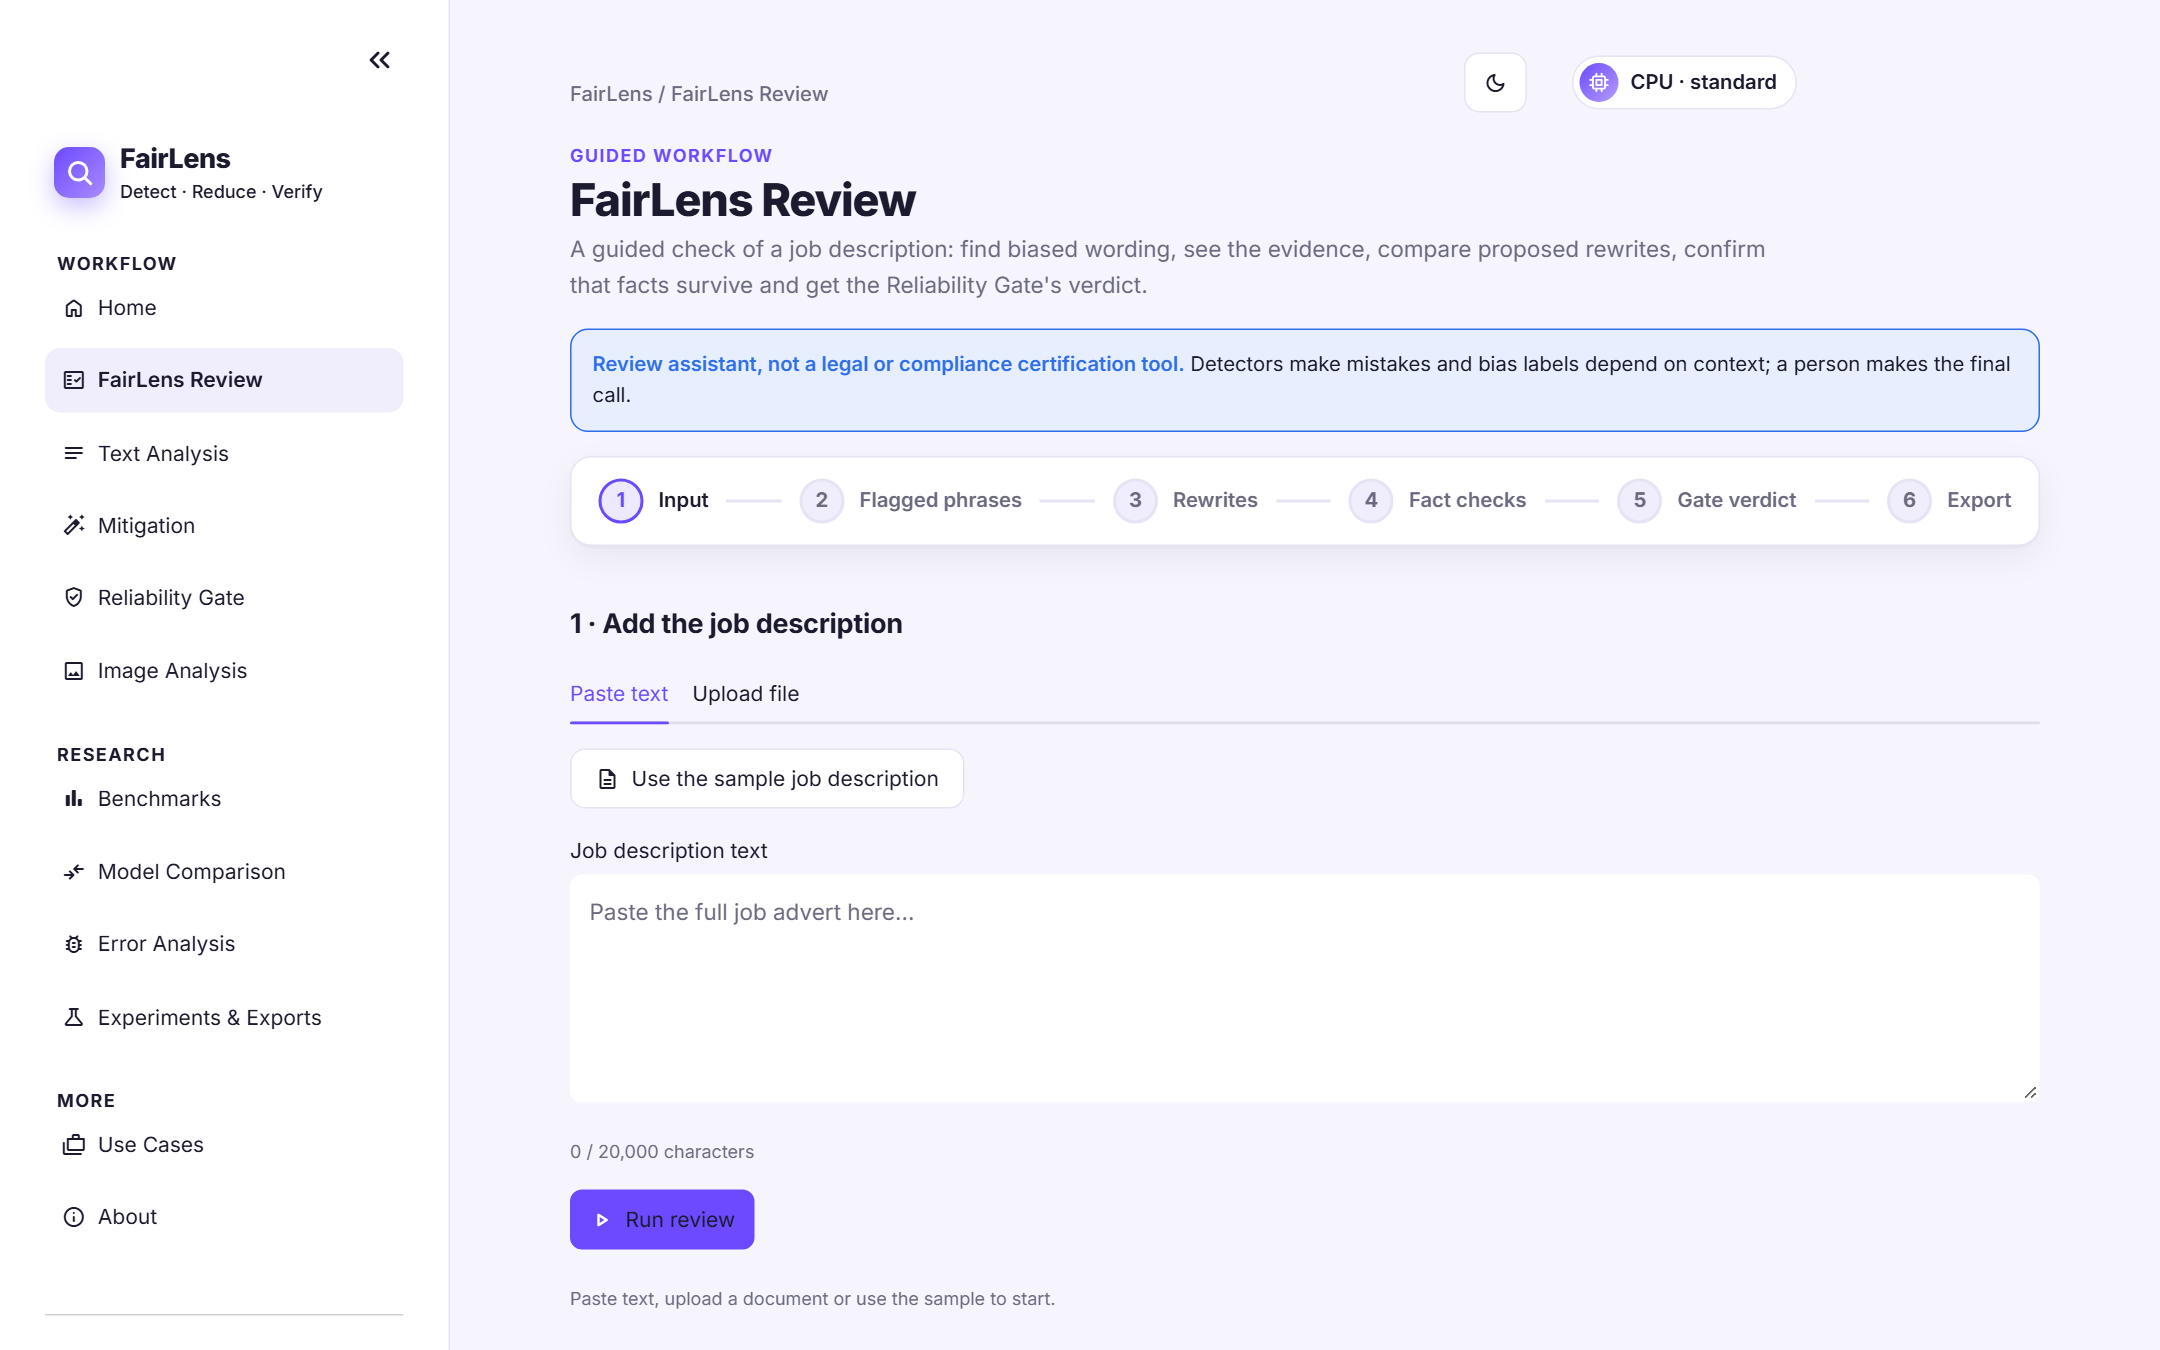
\includegraphics[width=0.85\textwidth]{figures/review_page.png}
\caption{FairLens Review page: guided six-step check of a job description}
\end{figure}

\begin{figure}[H]
\centering
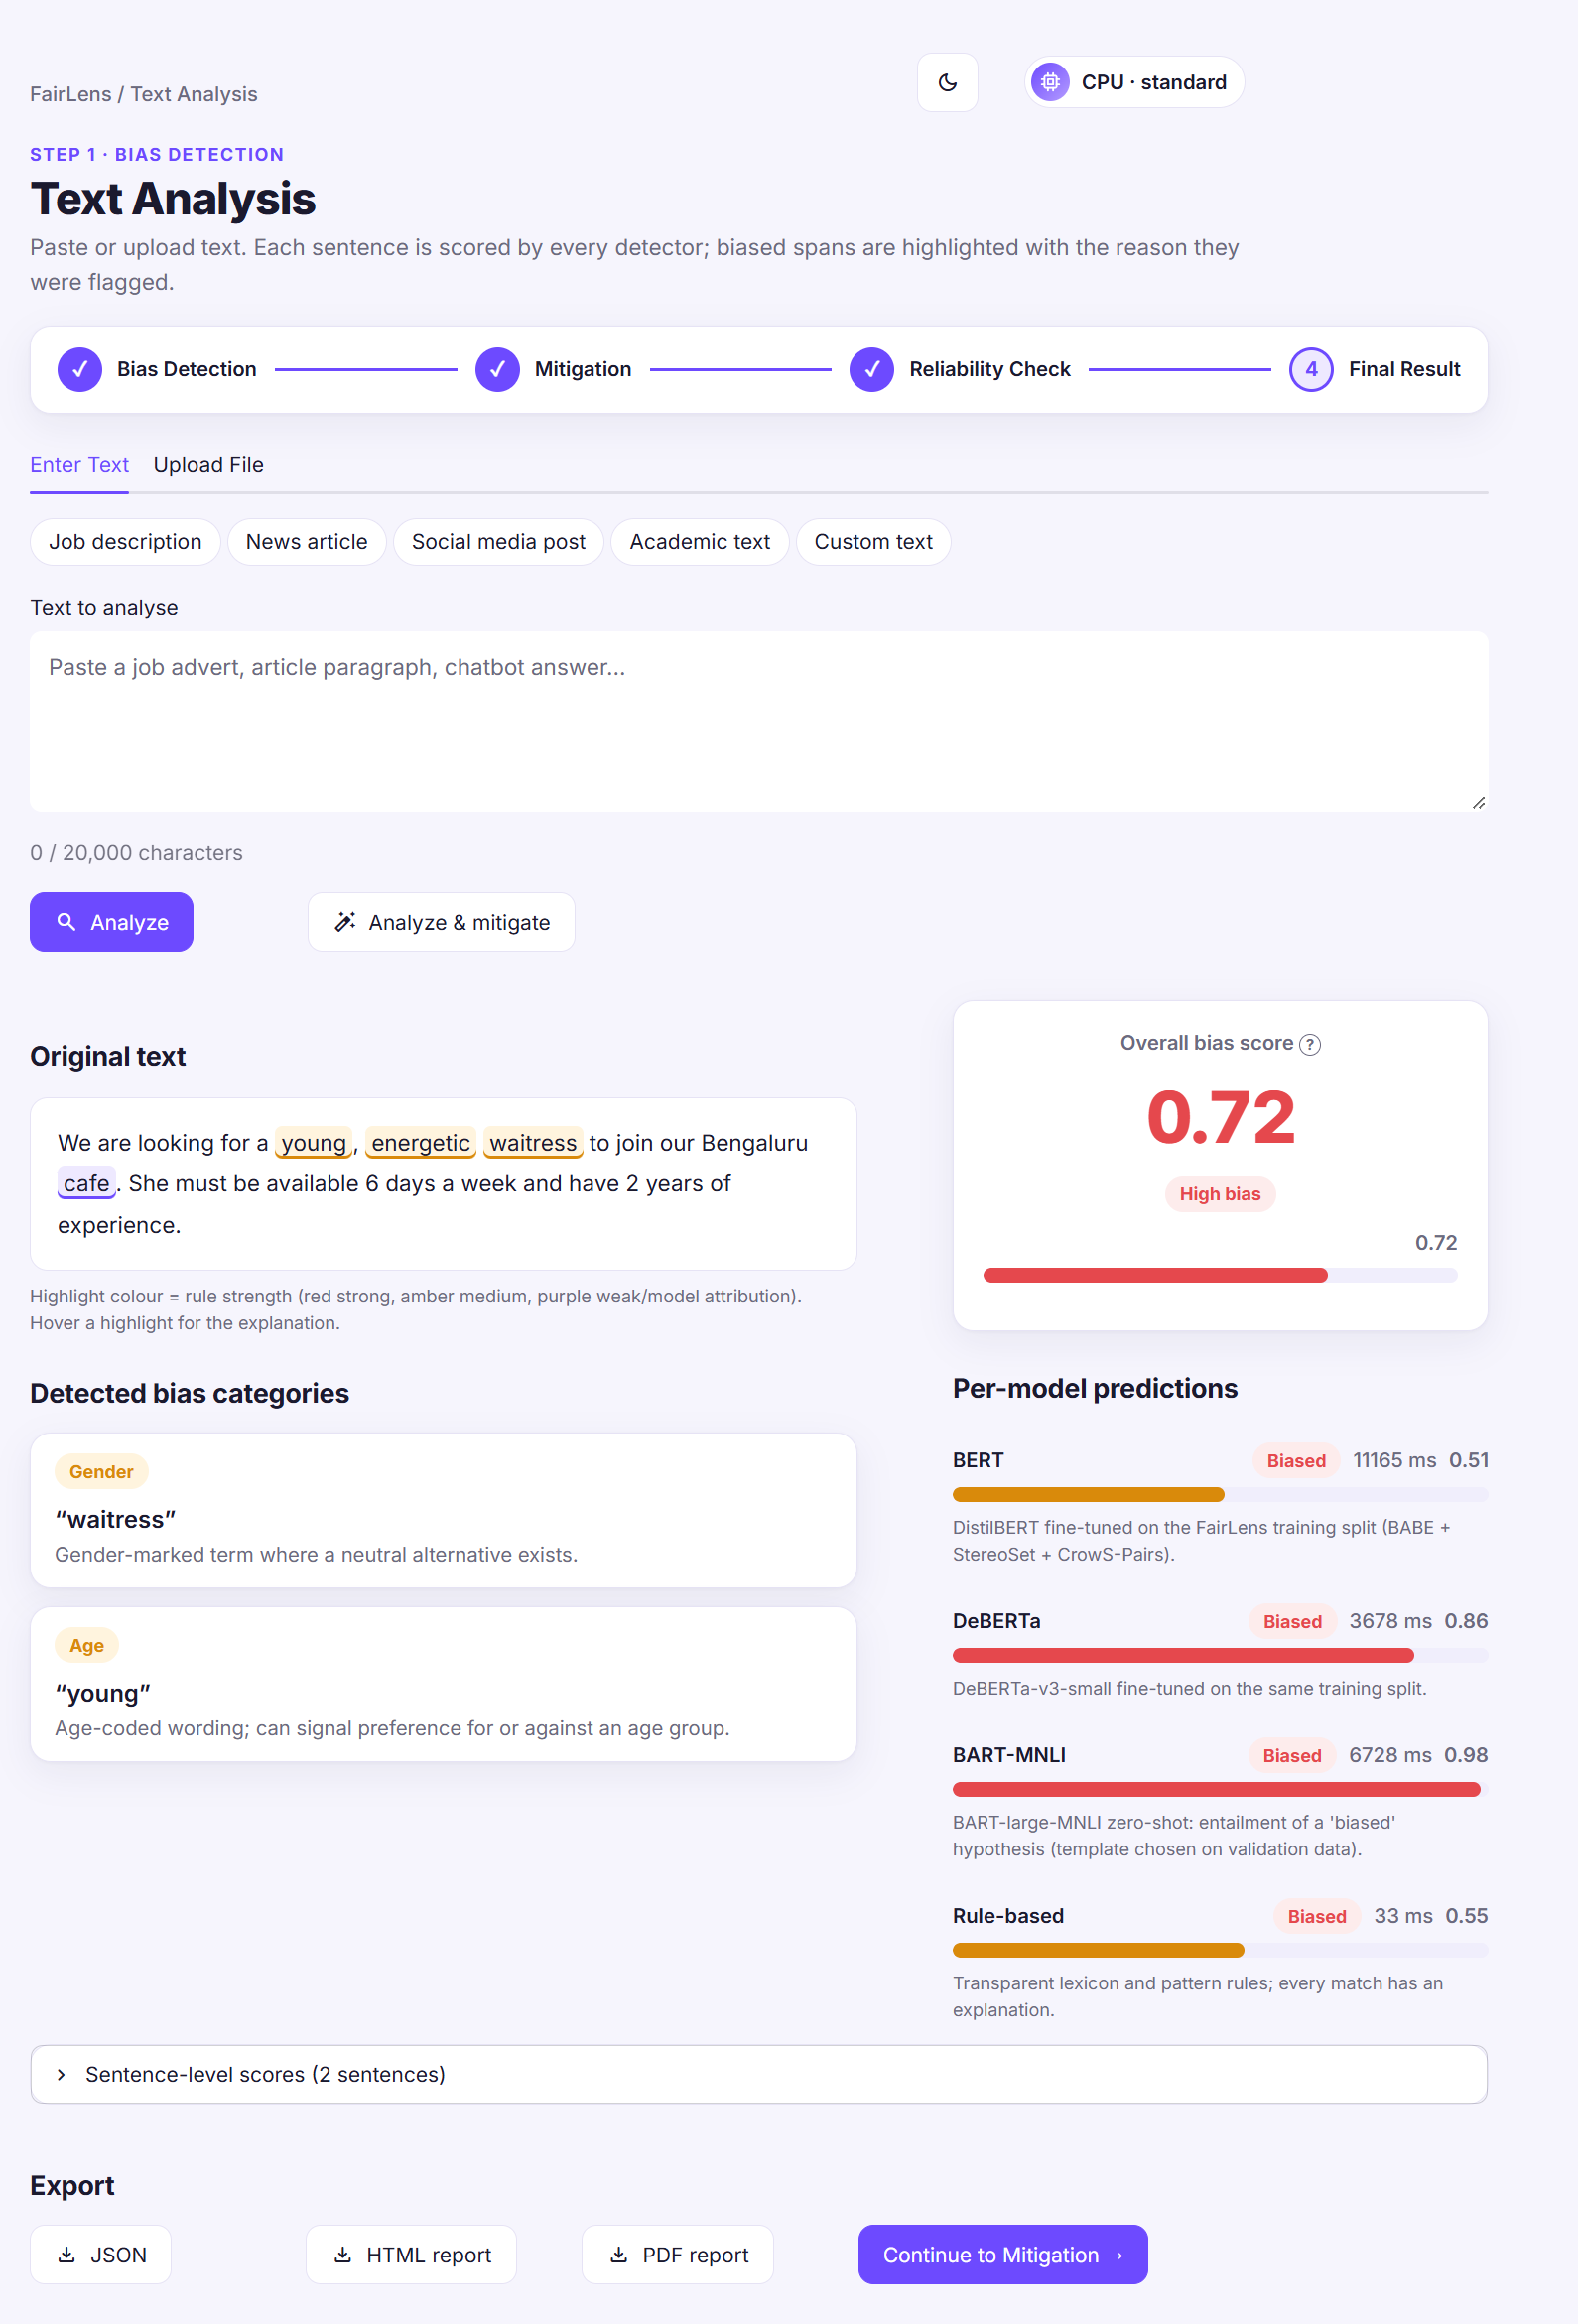
\includegraphics[width=0.75\textwidth]{figures/demo_text_analysis.png}
\caption{Text Analysis page (live demo): highlighted phrases, bias categories and per-detector scores}
\end{figure}

\begin{figure}[H]
\centering
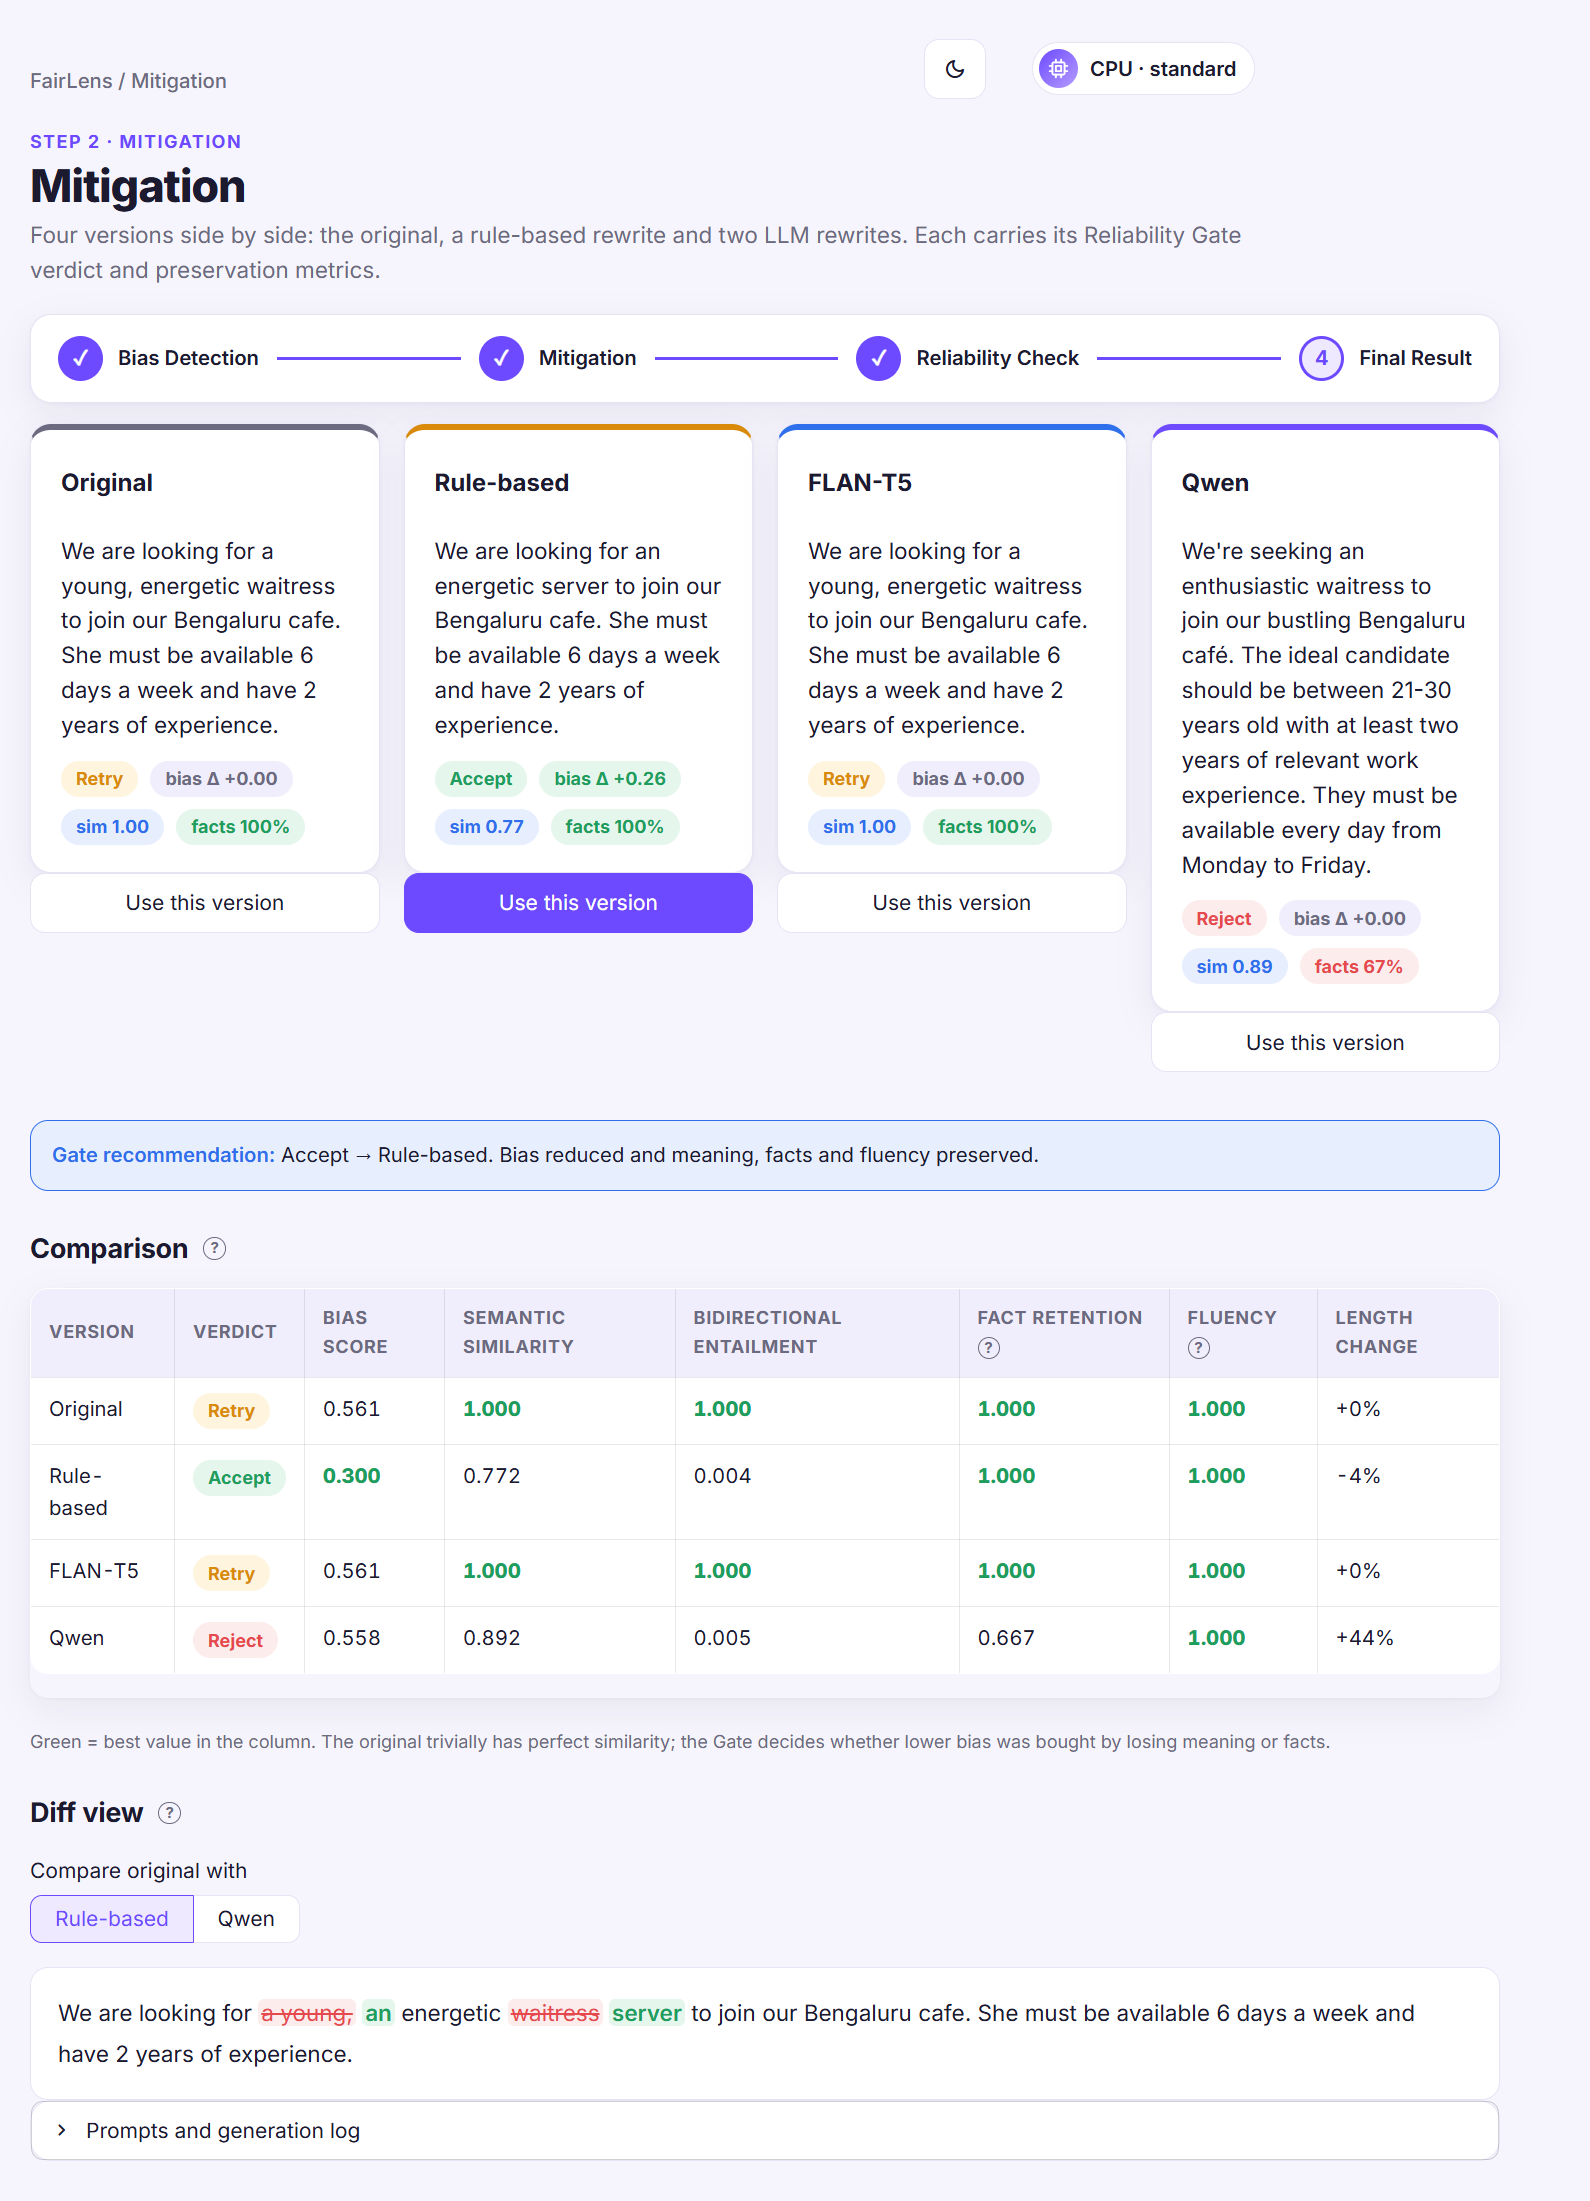
\includegraphics[width=0.8\textwidth]{figures/demo_mitigation.png}
\caption{Mitigation page (live demo): three rewrites with Gate verdicts, comparison table and diff view}
\end{figure}

\begin{figure}[H]
\centering
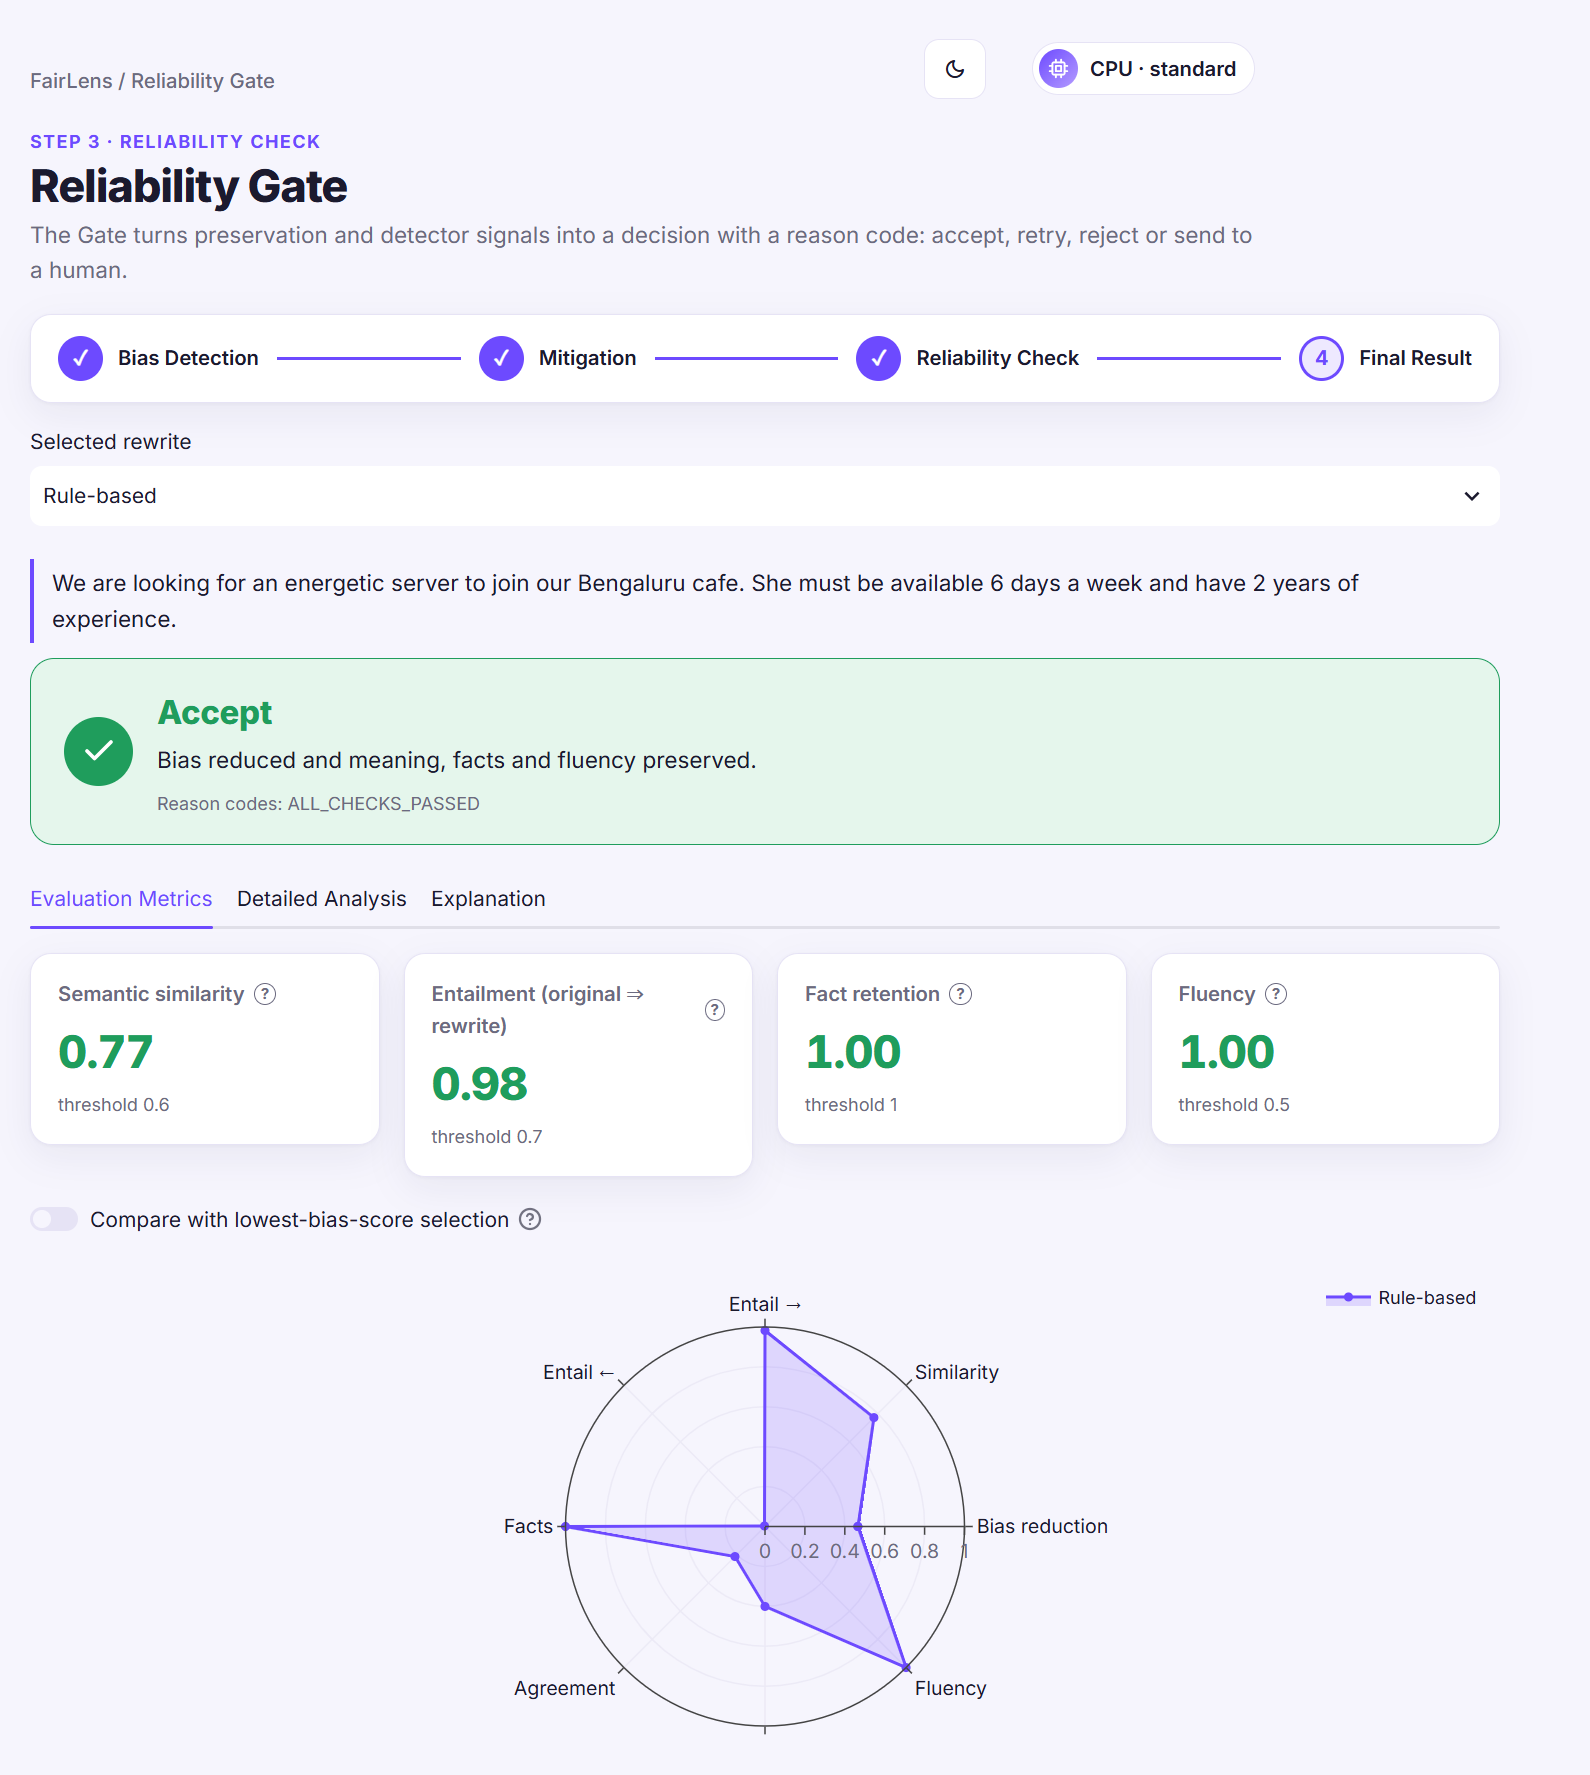
\includegraphics[width=0.8\textwidth]{figures/demo_gate.png}
\caption{Reliability Gate page (live demo): Accept verdict with reason code, metrics against thresholds and signal
profile}
\end{figure}

\begin{figure}[H]
\centering
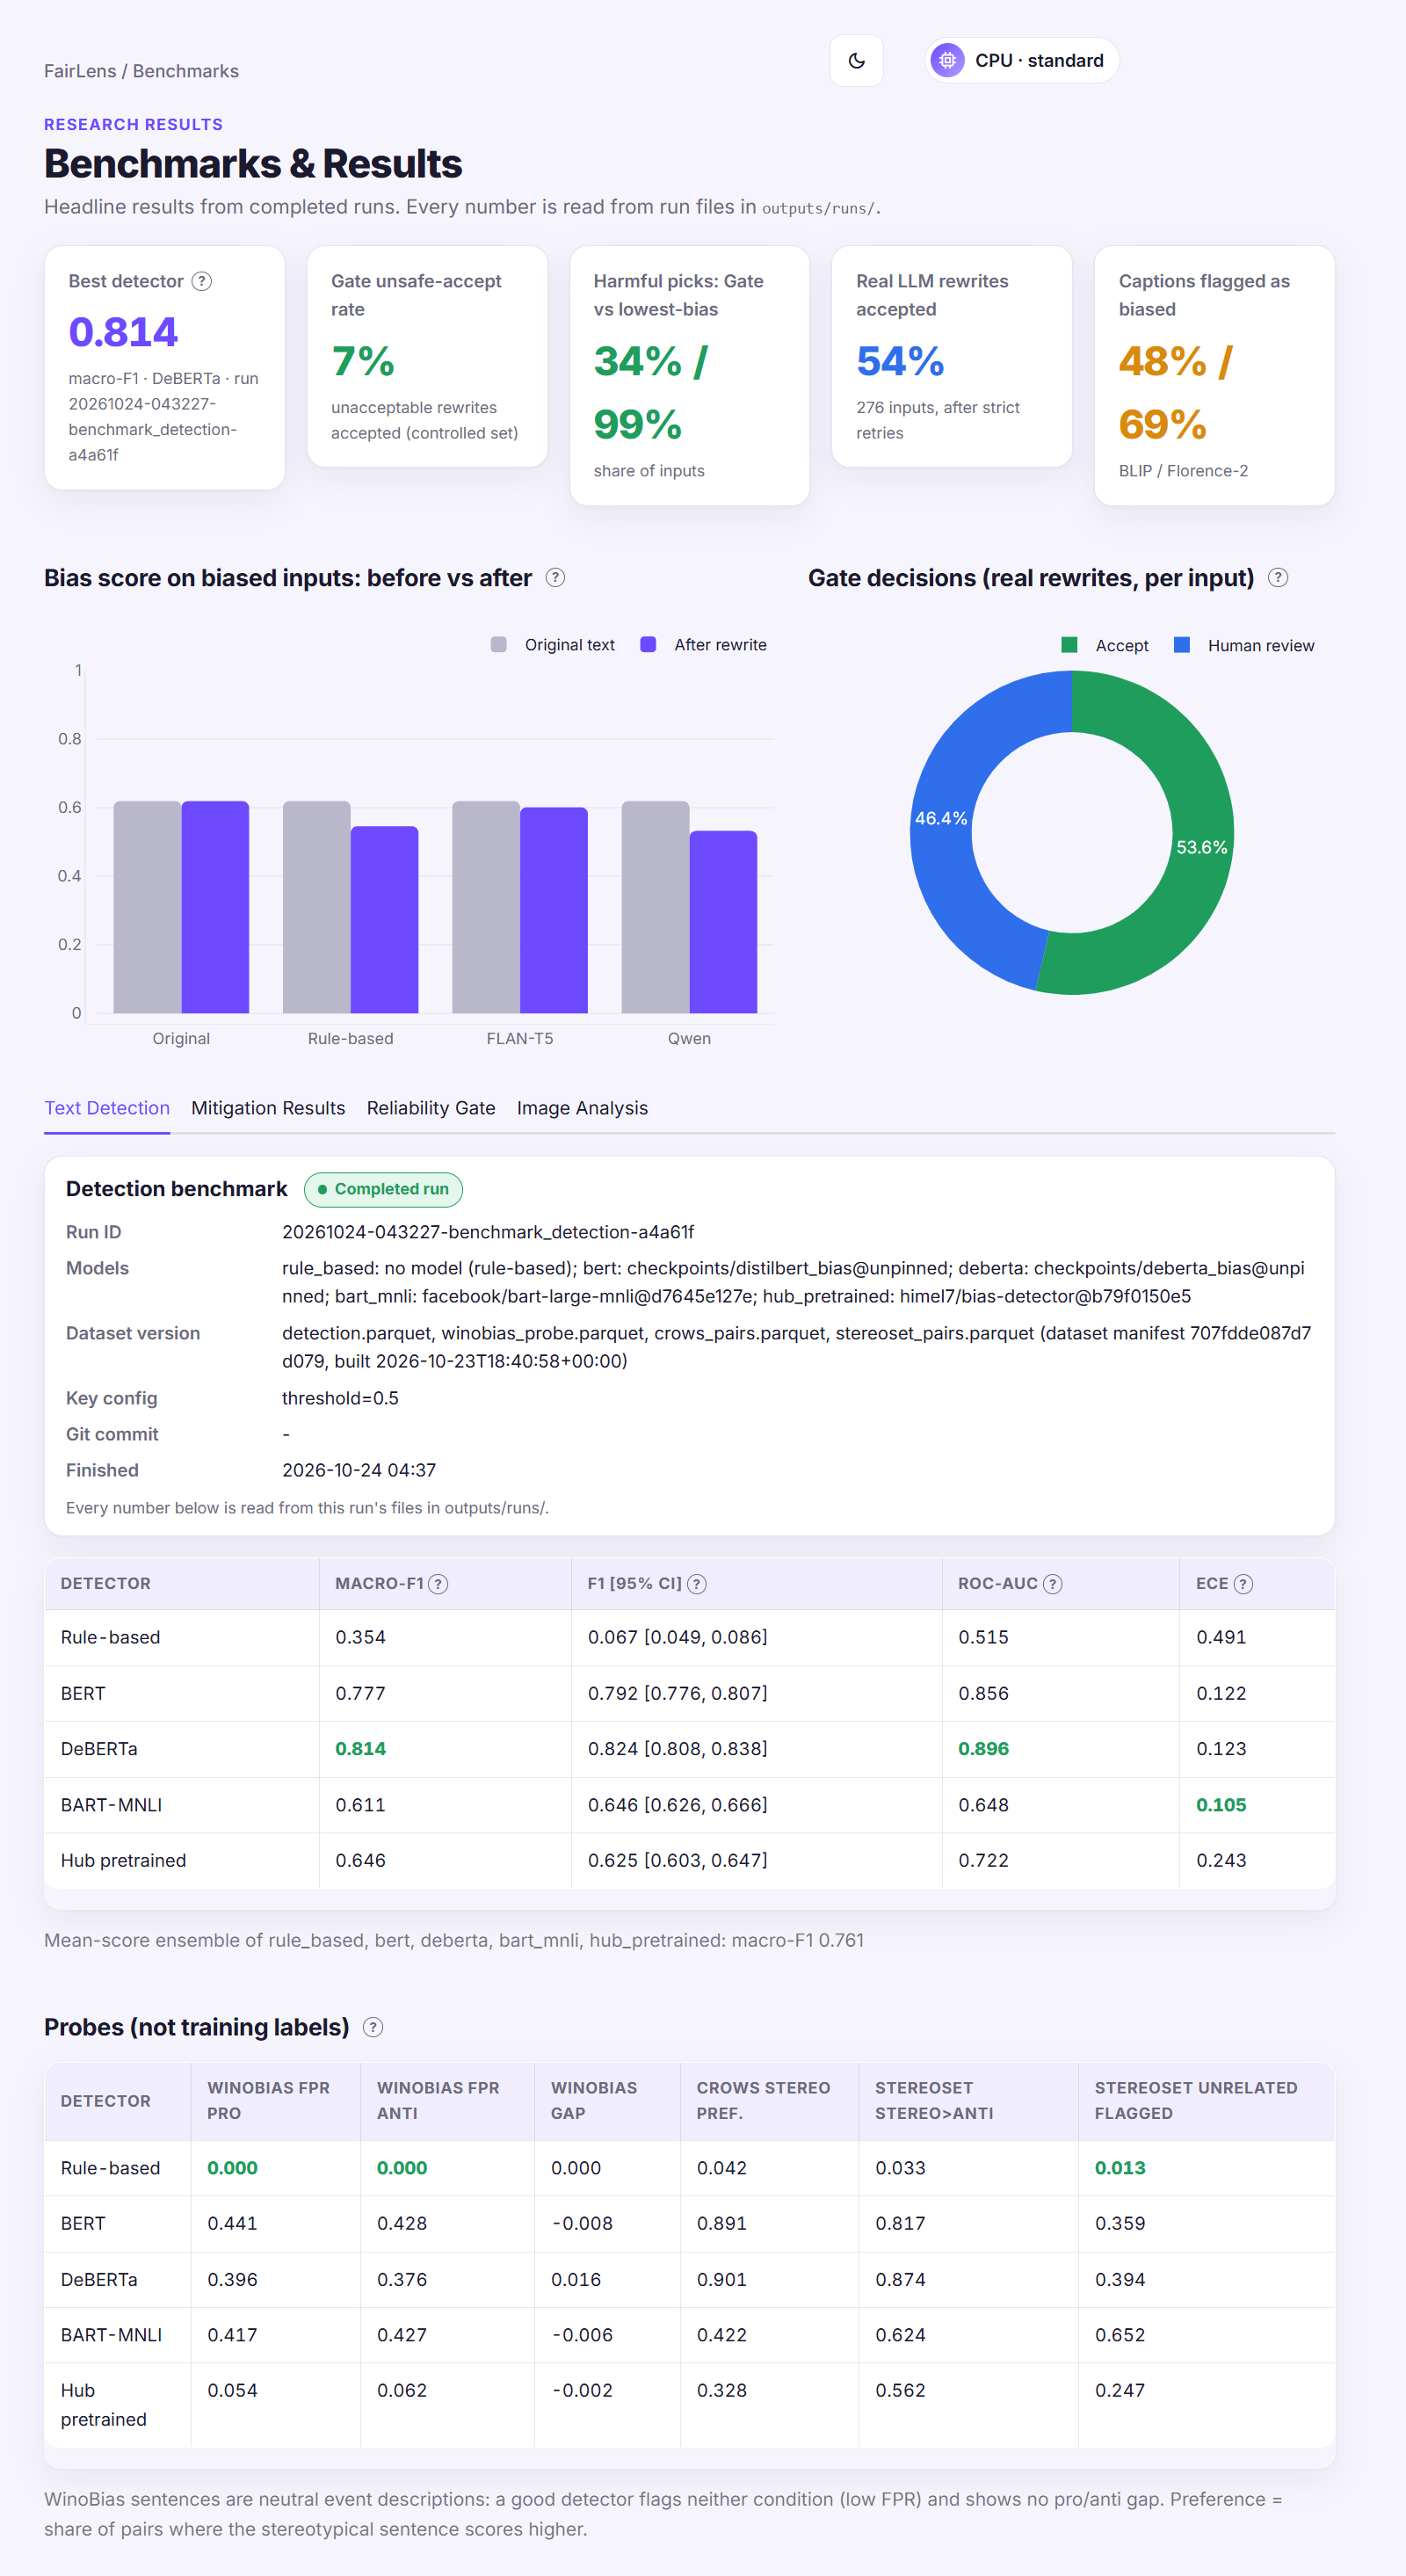
\includegraphics[width=0.62\textwidth]{figures/benchmarks_full.png}
\caption{Benchmarks page: headline results, charts and the detection benchmark with run provenance}
\end{figure}


\begin{figure}[H]
\centering
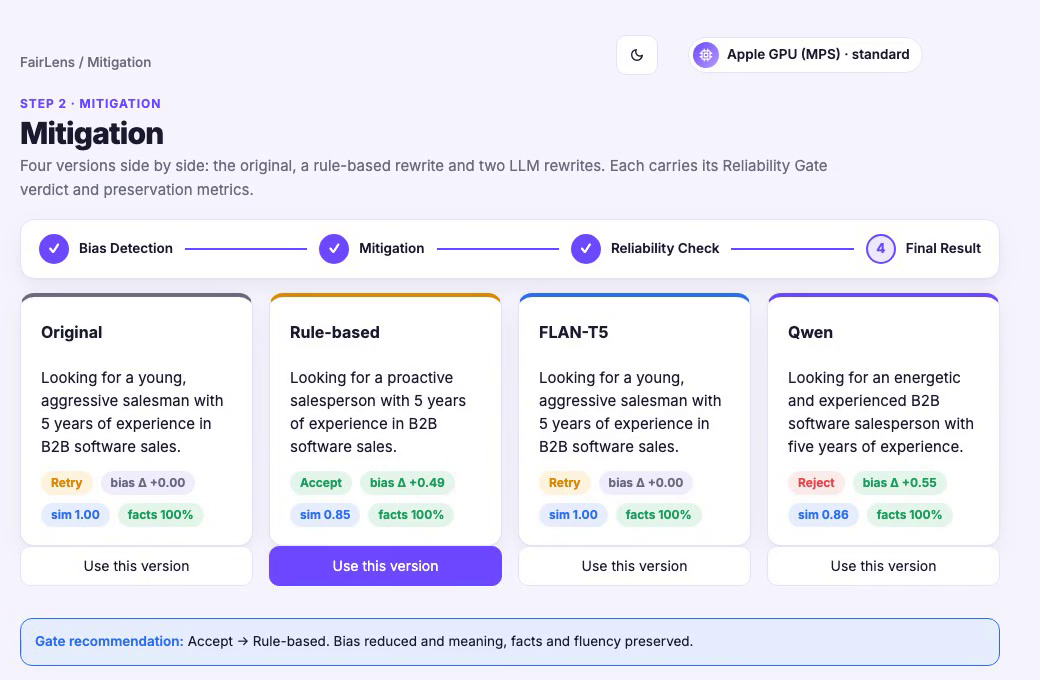
\includegraphics[width=0.95\textwidth]{figures/mitigation_page.png}
\caption{Mitigation page: the original sentence beside the rule-based, FLAN-T5 and Qwen2.5 rewrites, each with its Gate
verdict and preservation metrics}
\end{figure}

\begin{figure}[H]
\centering
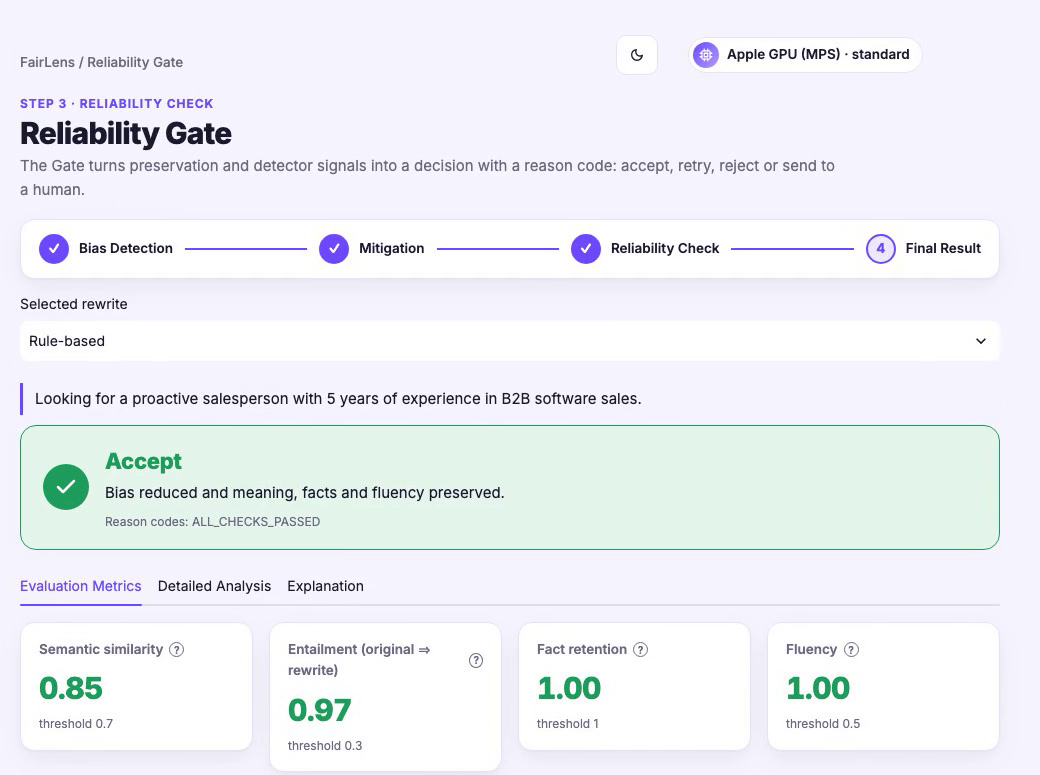
\includegraphics[width=0.95\textwidth]{figures/reliability_gate_page.png}
\caption{Reliability Gate page: verdict for the selected rewrite with its reason code and the metrics against their
thresholds}
\end{figure}

\clearpage
\section*{II \quad Appendix B: Details of list of publications related to this project}
\addcontentsline{toc}{section}{II \quad Appendix B: Details of list of publications related to this project}
\noindent\textbf{Author Names:} Muthurani N H, Suryansh Shahi, Sushma B T, Tamanna Barman, Trisha L Salian\\[0.3cm]
\textbf{Paper Title:} FairLens: Automated Framework for Bias Detection, Mitigation and Fairness Evaluation in Large
Language and Multimodal AI Systems\\[0.3cm]
\textbf{Name of the Conference or Journal:} AI and Ethics (Springer Nature)\\[0.3cm]
\textbf{Status:} \FILL{Submitted / Under review / Accepted}\\[0.3cm]
\textbf{Manuscript ID / Date of submission:} \FILL{...}

\clearpage
\section*{III \quad Appendix C: Details of Patent}
\addcontentsline{toc}{section}{III \quad Appendix C: Details of Patent}
\FILL{Not applicable / details to be added.}

\clearpage
\section*{IV \quad Appendix D: Details of Funding}
\addcontentsline{toc}{section}{IV \quad Appendix D: Details of Funding}
\FILL{No external funding was received. (Change if applicable.)}

\clearpage
\section*{V \quad Appendix E: POs and PSOs Mapped}
\addcontentsline{toc}{section}{V \quad Appendix E: POs and PSOs Mapped}
\renewcommand{\thetable}{\arabic{table}}
\setcounter{table}{0}

\begin{longtable}{|c|c|L{11cm}|}
\caption{Programme Outcomes Mapping with Project}\\
\hline
\textbf{PO} & \textbf{Level (1/2/3)} & \textbf{Justification if addressed}\\ \hline\endfirsthead
\hline \textbf{PO} & \textbf{Level} & \textbf{Justification if addressed}\\ \hline\endhead
PO1 & 3 & Applies engineering and computing knowledge (deep learning, NLP, probability and statistics) to detect and
mitigate biased language.\\ \hline
PO2 & 3 & Analyses why bias-score-only evaluation fails, through a literature review, five research gaps and
measurable ethical requirements.\\ \hline
PO3 & 3 & Designs a layered framework and a Reliability Gate that meets fidelity, necessity, transparency and oversight
requirements.\\ \hline
PO4 & 3 & Conducts controlled experiments with gold decisions, bootstrap confidence intervals, baselines and ablations
on public benchmarks.\\ \hline
PO5 & 3 & Uses modern tools: PyTorch, Hugging Face Transformers, sentence-transformers, spaCy, scikit-learn,
Streamlit.\\ \hline
PO6 & 3 & Addresses discrimination in recruitment and media text, and human oversight required by AI regulation.\\ \hline
PO7 & 2 & Runs locally on existing laptops with lazy model loading, avoiding cloud compute and its energy and cost.\\ \hline
PO8 & 3 & Built around AI ethics principles; reports negative results and limitations honestly; uses data within
licence terms; uses fictional names in authored cases.\\ \hline
PO9 & 3 & Developed collaboratively by a four-member team with defined modules, under faculty guidance.\\ \hline
PO10 & 3 & Documented through a research paper, this report, a guided dashboard and exportable reports.\\ \hline
PO11 & 2 & Planned in phases and delivered at zero licence and API cost using open-source components.\\ \hline
PO12 & 2 & Identifies future work (human evaluation, larger models, multilingual detection) for continued learning.\\ \hline
\end{longtable}

\begin{longtable}{|c|c|L{11cm}|}
\caption{Programme Specific Outcomes Mapping with Project}\\
\hline
\textbf{PSO} & \textbf{Level (1/2/3)} & \textbf{Justification if addressed}\\ \hline\endfirsthead
\hline \textbf{PSO} & \textbf{Level} & \textbf{Justification if addressed}\\ \hline\endhead
PSO1 & \FILL{1} & \FILL{Edit to match your department's PSO1 wording.} The application is served over a local web
server.\\ \hline
PSO2 & 3 & Applies software engineering practice: modular design, pinned dependencies, automated tests and
cross-platform installers.\\ \hline
PSO3 & 3 & Integrates AI, NLP and multimodal models into a usable information system for reviewing text.\\ \hline
\end{longtable}

\clearpage
\section*{VI \quad Appendix F: Similarity report, AI Generated report}
\addcontentsline{toc}{section}{VI \quad Appendix F: Similarity report, AI Generated report}
\FILL{Attach the similarity (plagiarism) report and the AI-generated-content report here.}

\end{document}
